One of the statistical method (CLs) used in this analysis for data
interpretation is based on a maximum likelihood fit that takes into
account the shapes of the discriminating variables. The fit can be
used to check how well the data matches background estimations. We use
the nominal configuration that combines the shape analysis in 0 and 1
jet channels with a cut based VBF analysis.

Two types of fits are performed. For the first one we fix the signal
yield to zero and fit data. The parameters of the model (nuisance
parameters) are going to be adjusted to accomodate the difference
between data and the expected background estimations. For the second
type of fits the signal yield is
unconstrained. Figures~\ref{fig:fit_115}-\ref{fig:fit_400} show
distributions of the BDT output for a few key mass
points. Figures~\ref{fig:bdt2_115}-\ref{fig:bdt2_400} show how the
distributions change for dominant backgrounds.

Overall the shapes are not changing much in the fits. \WW\
normalization is often changed to compensate for an excess in the
background only fits at low mass. At high mass we see a systematic
shift for the \WW\ normalization in all channels both for background
only and signal+background fits. In the high Higgs mass case we don't
use a data driven estimation for \WW\ contribution and rely completely
on Monte Carlo. For the low mass Higgs we see roughly 15\% more \WW\
events in data than in Monte Carlo. The shift observed in the fits at
high mass is consistent with this estimate. This observation suggests
that the fit can extract the \WW\ component from data using the
difference in the shape of different background contributions.

\begin{figure}[!hbtp]
\centering
\subfigure[$e\mu$ 0-Jet]{
\centering
\label{subfig:c3_115_n0of}
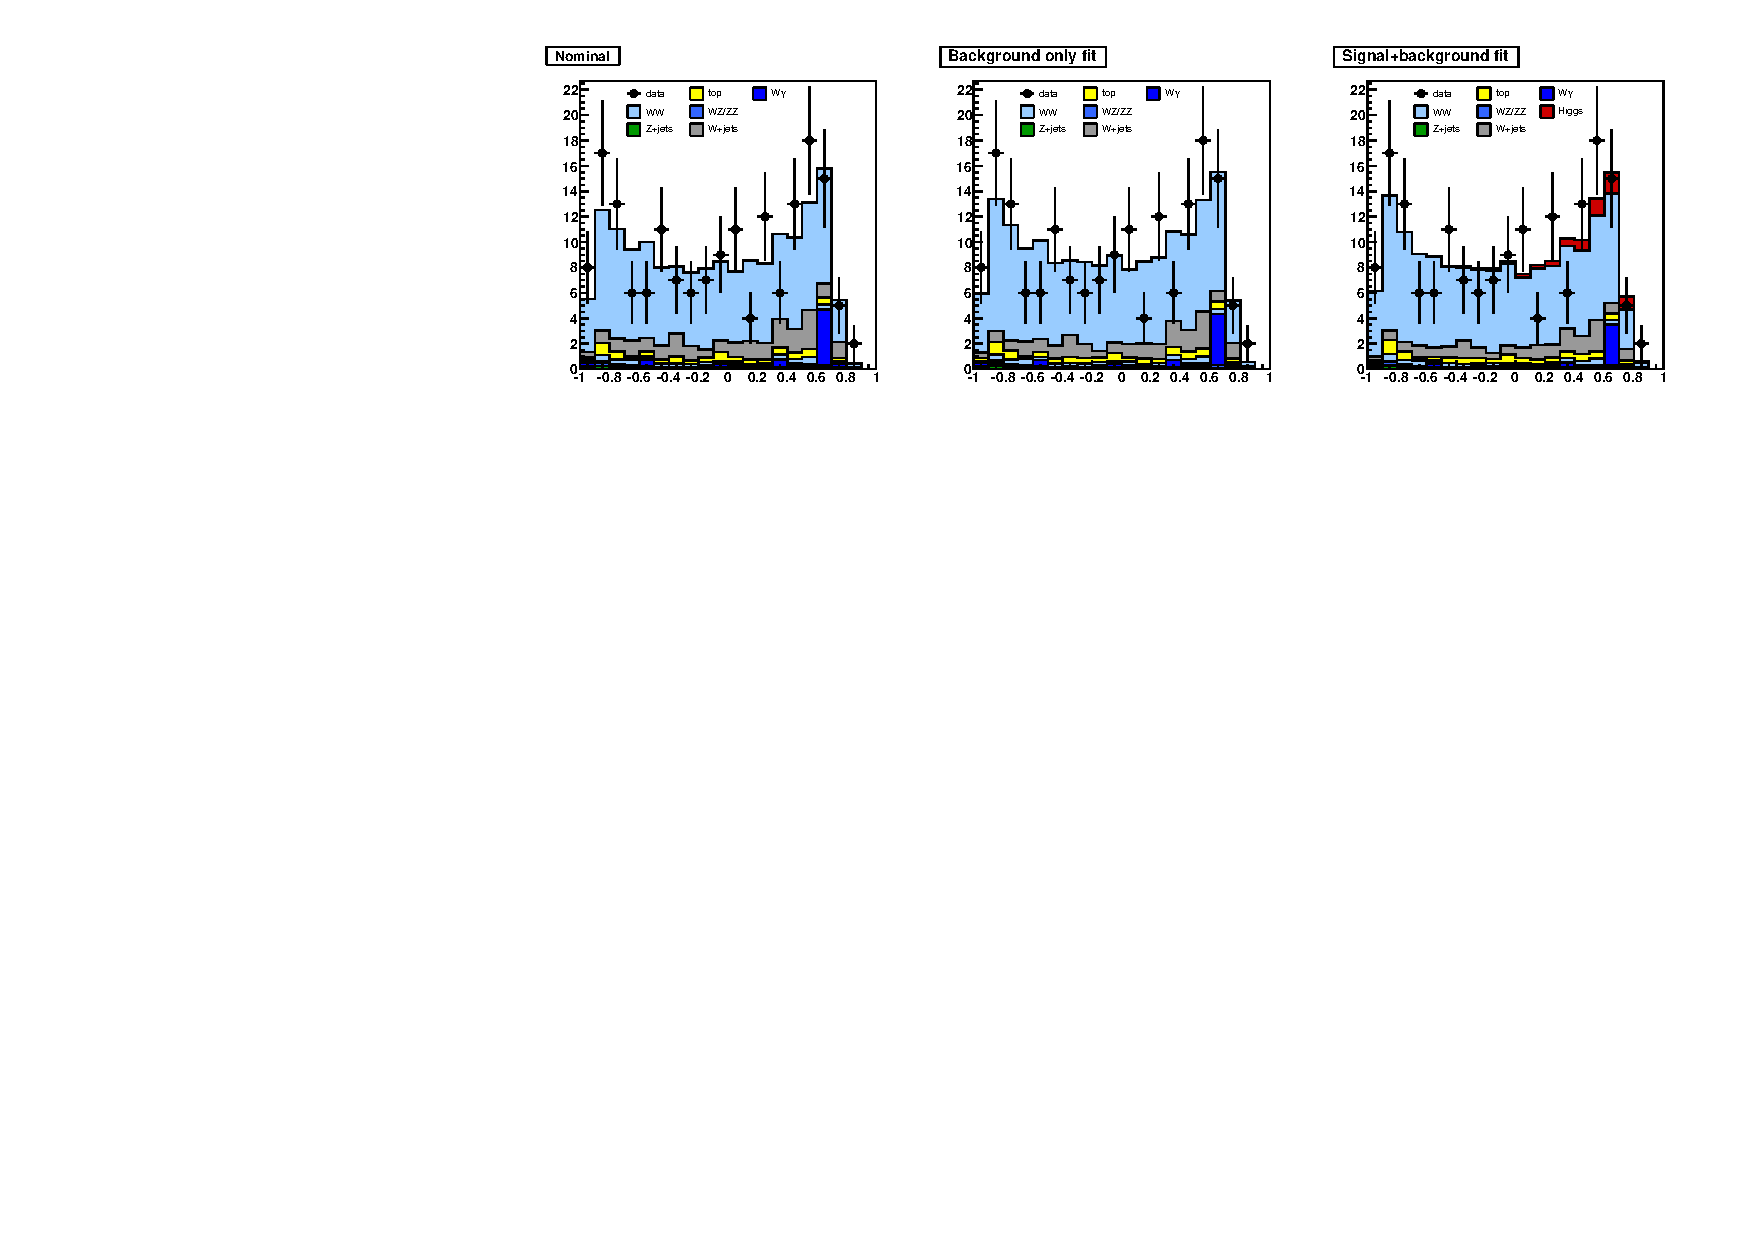
\includegraphics[width=0.9\textwidth]{figures/fits/bdt_115_n0of.pdf}}\\
\subfigure[$ee$/$\mu\mu$ 0-Jet]{
\centering
\label{subfig:bdt_115_n0sf}
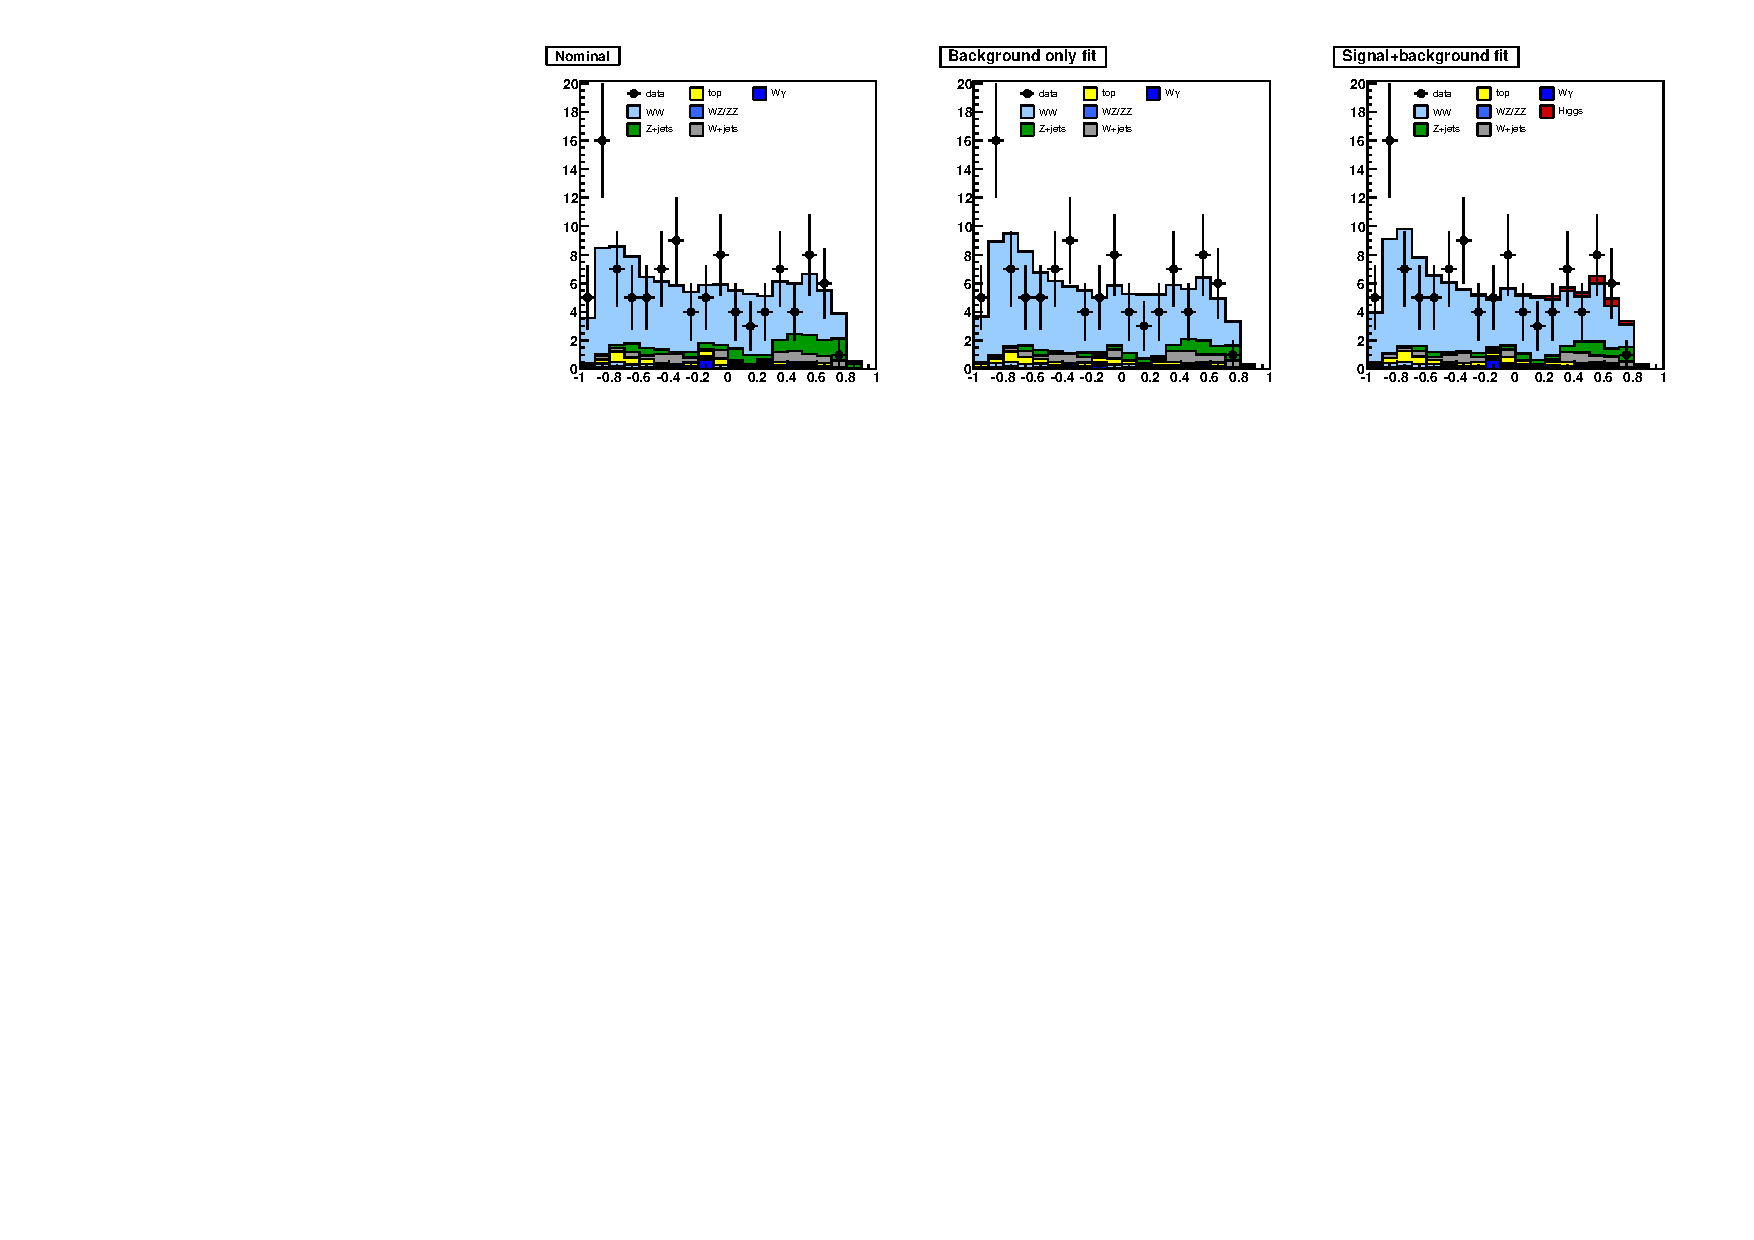
\includegraphics[width=0.9\textwidth]{figures/fits/bdt_115_n0sf.pdf}}
\subfigure[$e\mu$ 1-Jet]{
\centering
\label{subfig:bdt_115_n1of}
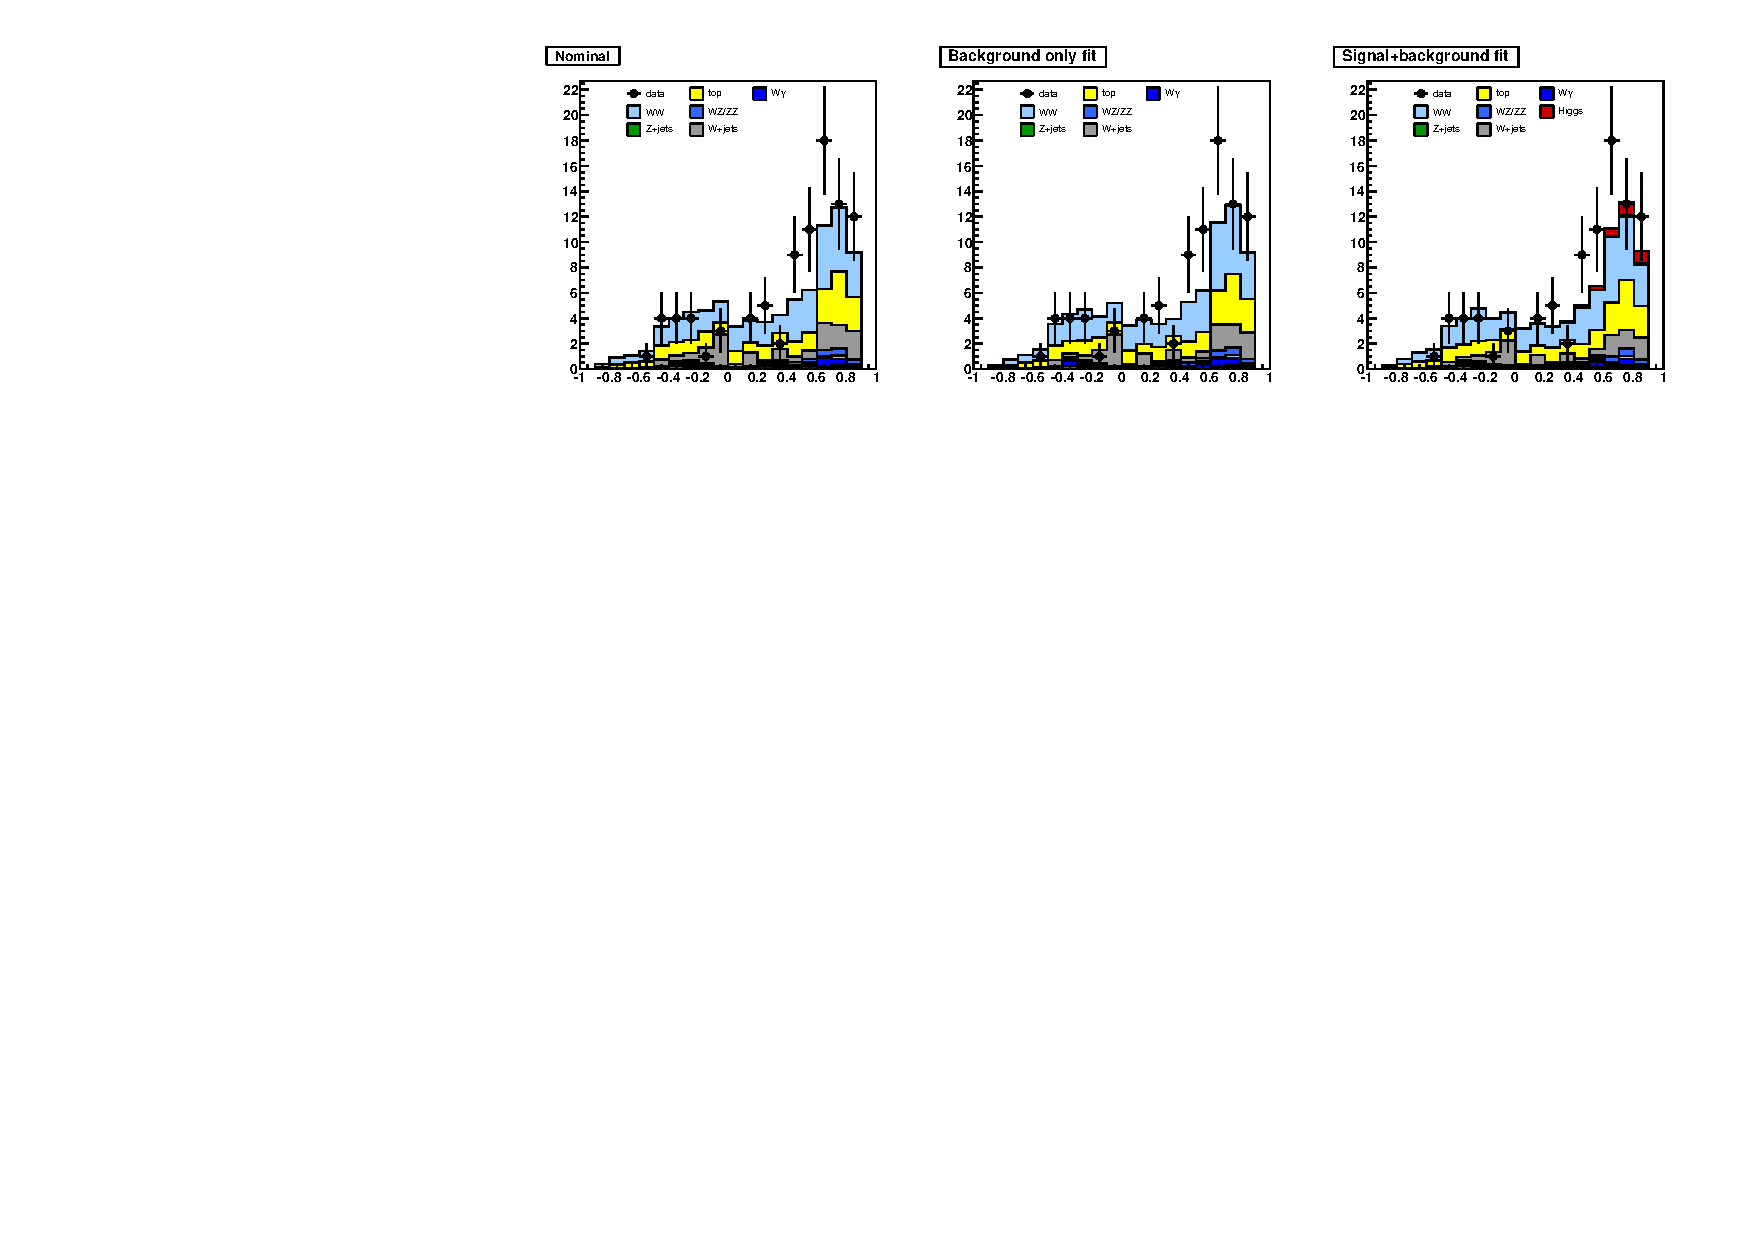
\includegraphics[width=0.9\textwidth]{figures/fits/bdt_115_n1of.pdf}}
\subfigure[$ee$/$\mu\mu$ 1-Jet]{
\centering
\label{subfig:bdt_115_n1sf}
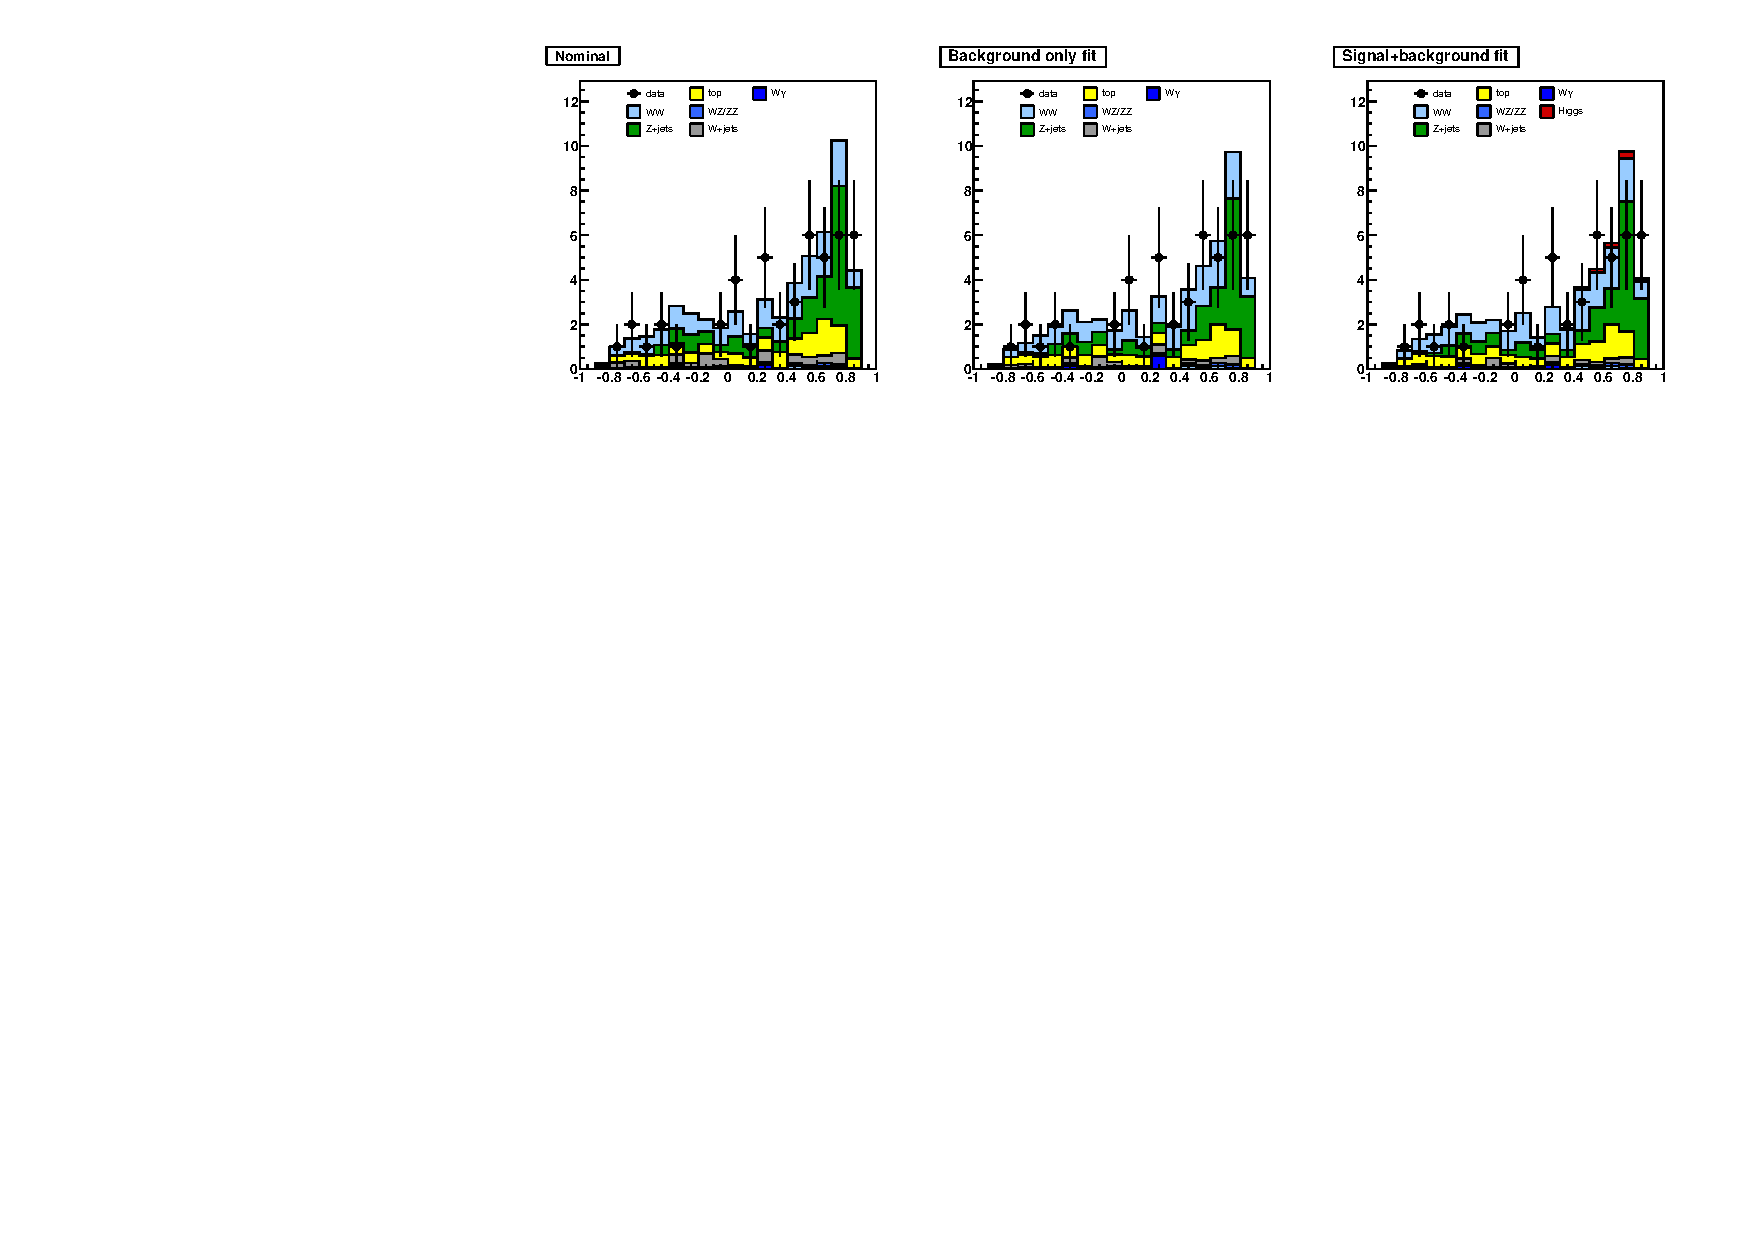
\includegraphics[width=0.9\textwidth]{figures/fits/bdt_115_n1sf.pdf}}
\caption{
MVA output distributions for Higgs 115~\GeV\ without fitting
(nominal), background fit (signal is set to zero) and
signal+background fit (signal is floating in the fit). Signal strength
for the signal+background fit is found to be 2.1 with 68\% CL range:
[0.8,3.6] }
\label{fig:fit_115}
\end{figure}

\begin{figure}[!hbtp]
\centering
\subfigure[$e\mu$ 0-Jet]{
\centering
\label{subfig:c3_120_n0of}
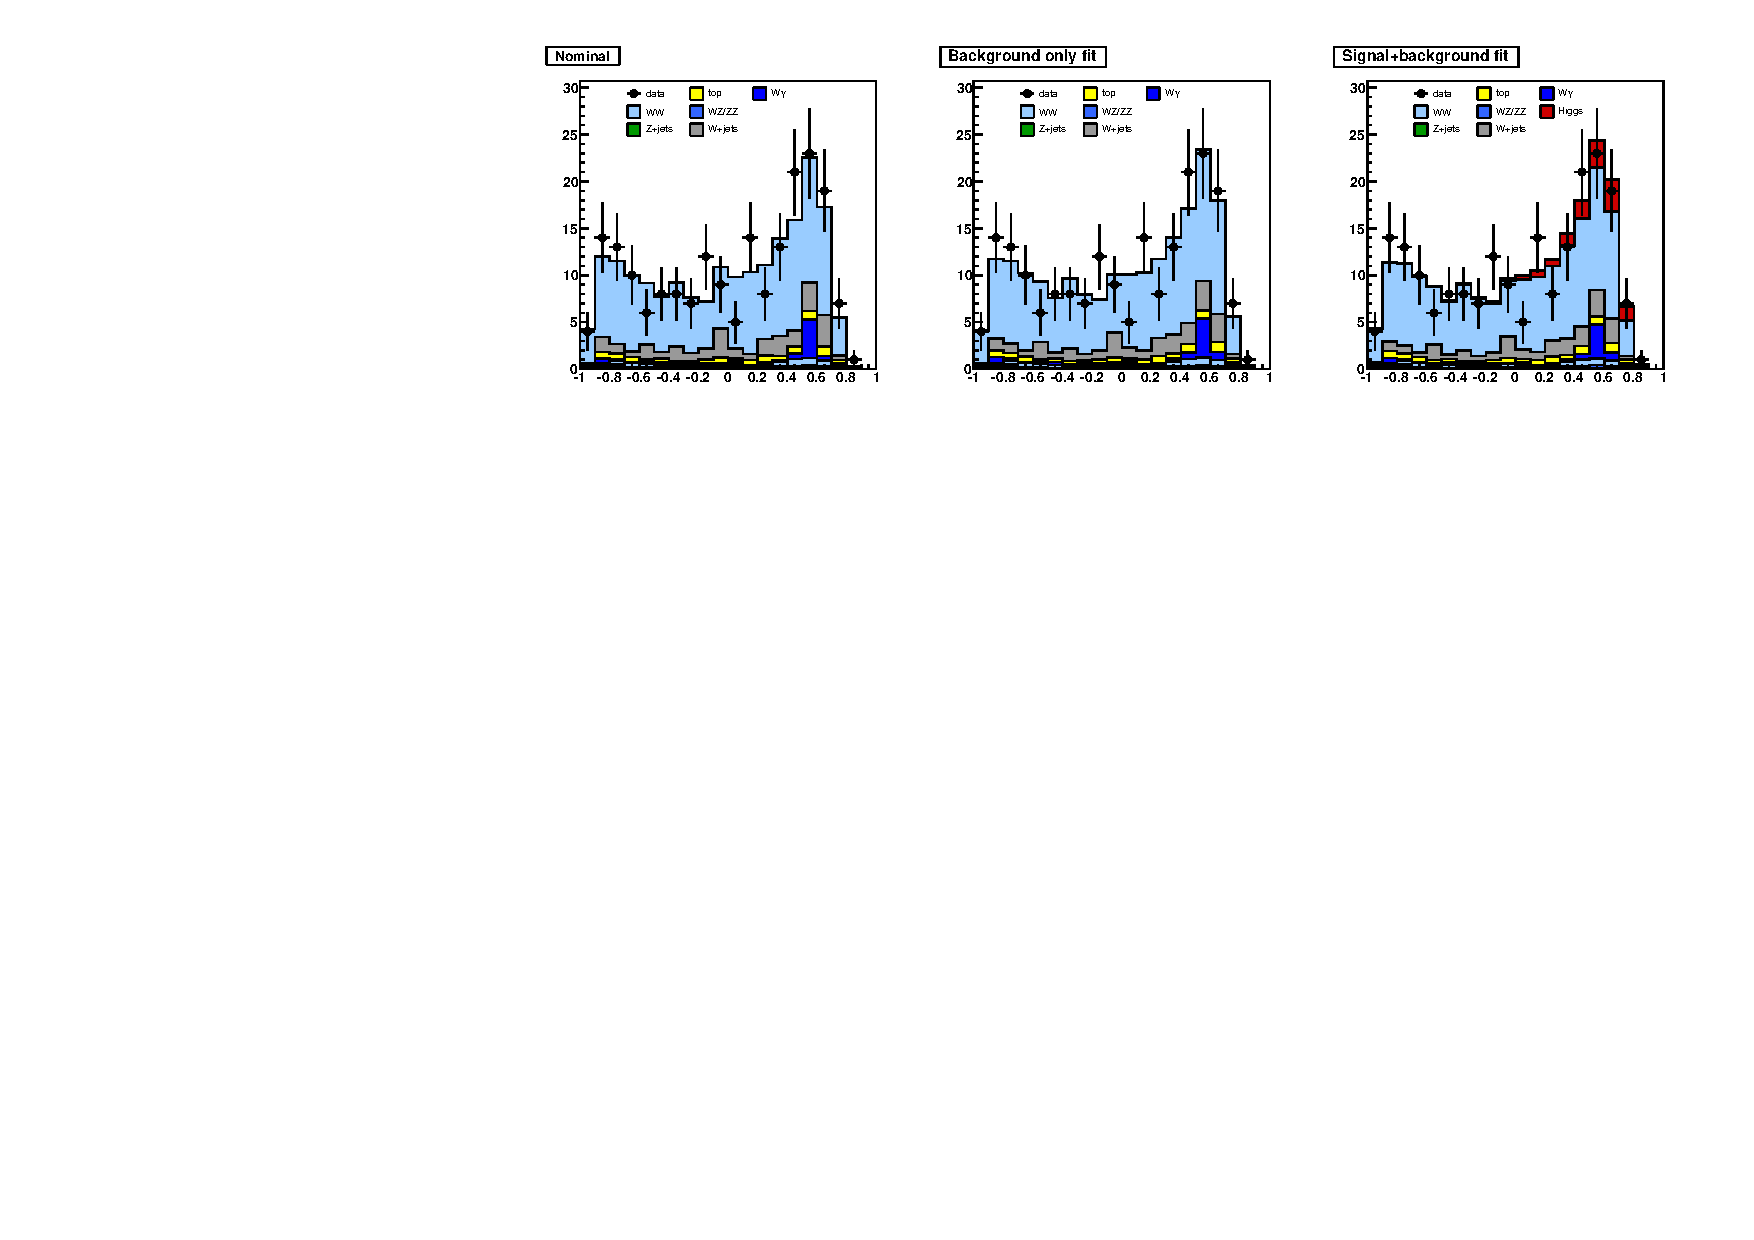
\includegraphics[width=0.9\textwidth]{figures/fits/bdt_120_n0of.pdf}}\\
\subfigure[$ee$/$\mu\mu$ 0-Jet]{
\centering
\label{subfig:bdt_120_n0sf}
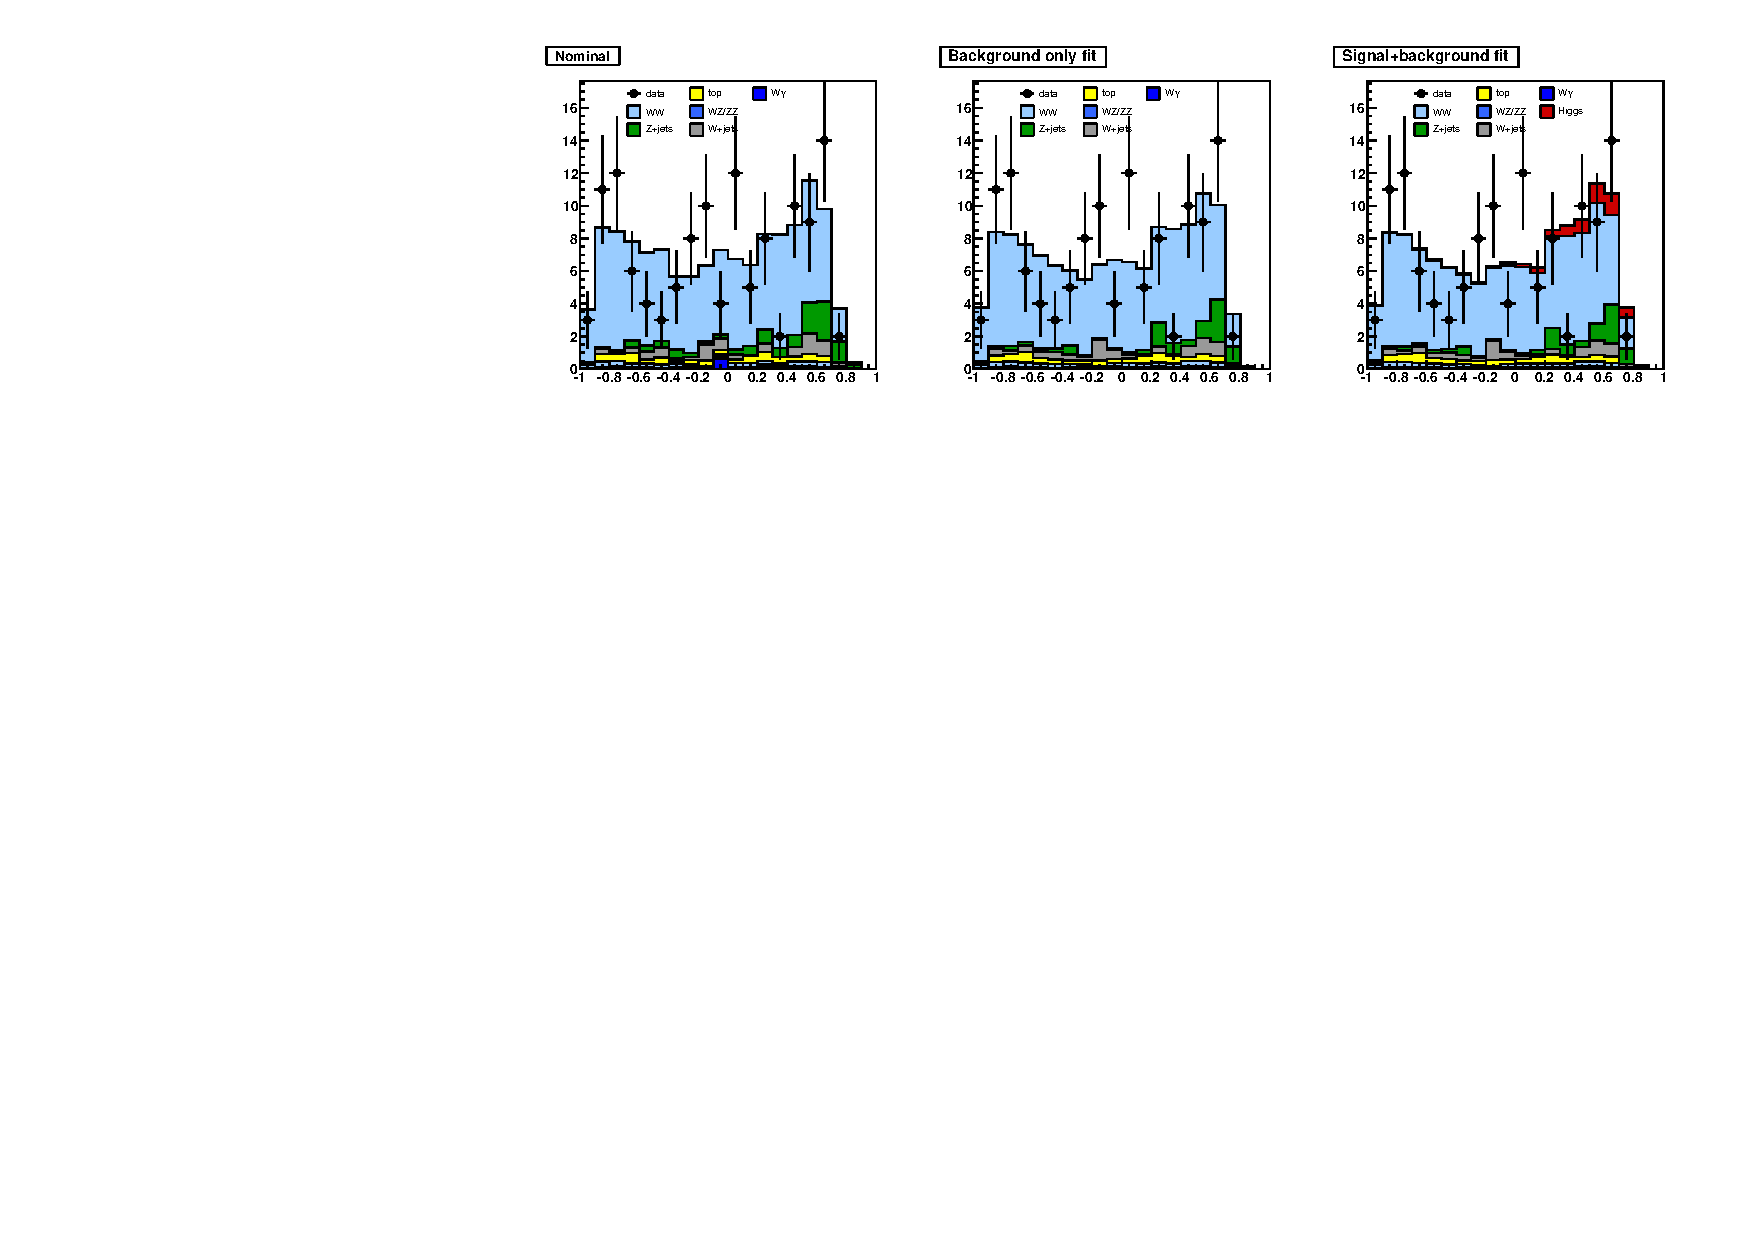
\includegraphics[width=0.9\textwidth]{figures/fits/bdt_120_n0sf.pdf}}
\subfigure[$e\mu$ 1-Jet]{
\centering
\label{subfig:bdt_120_n1of}
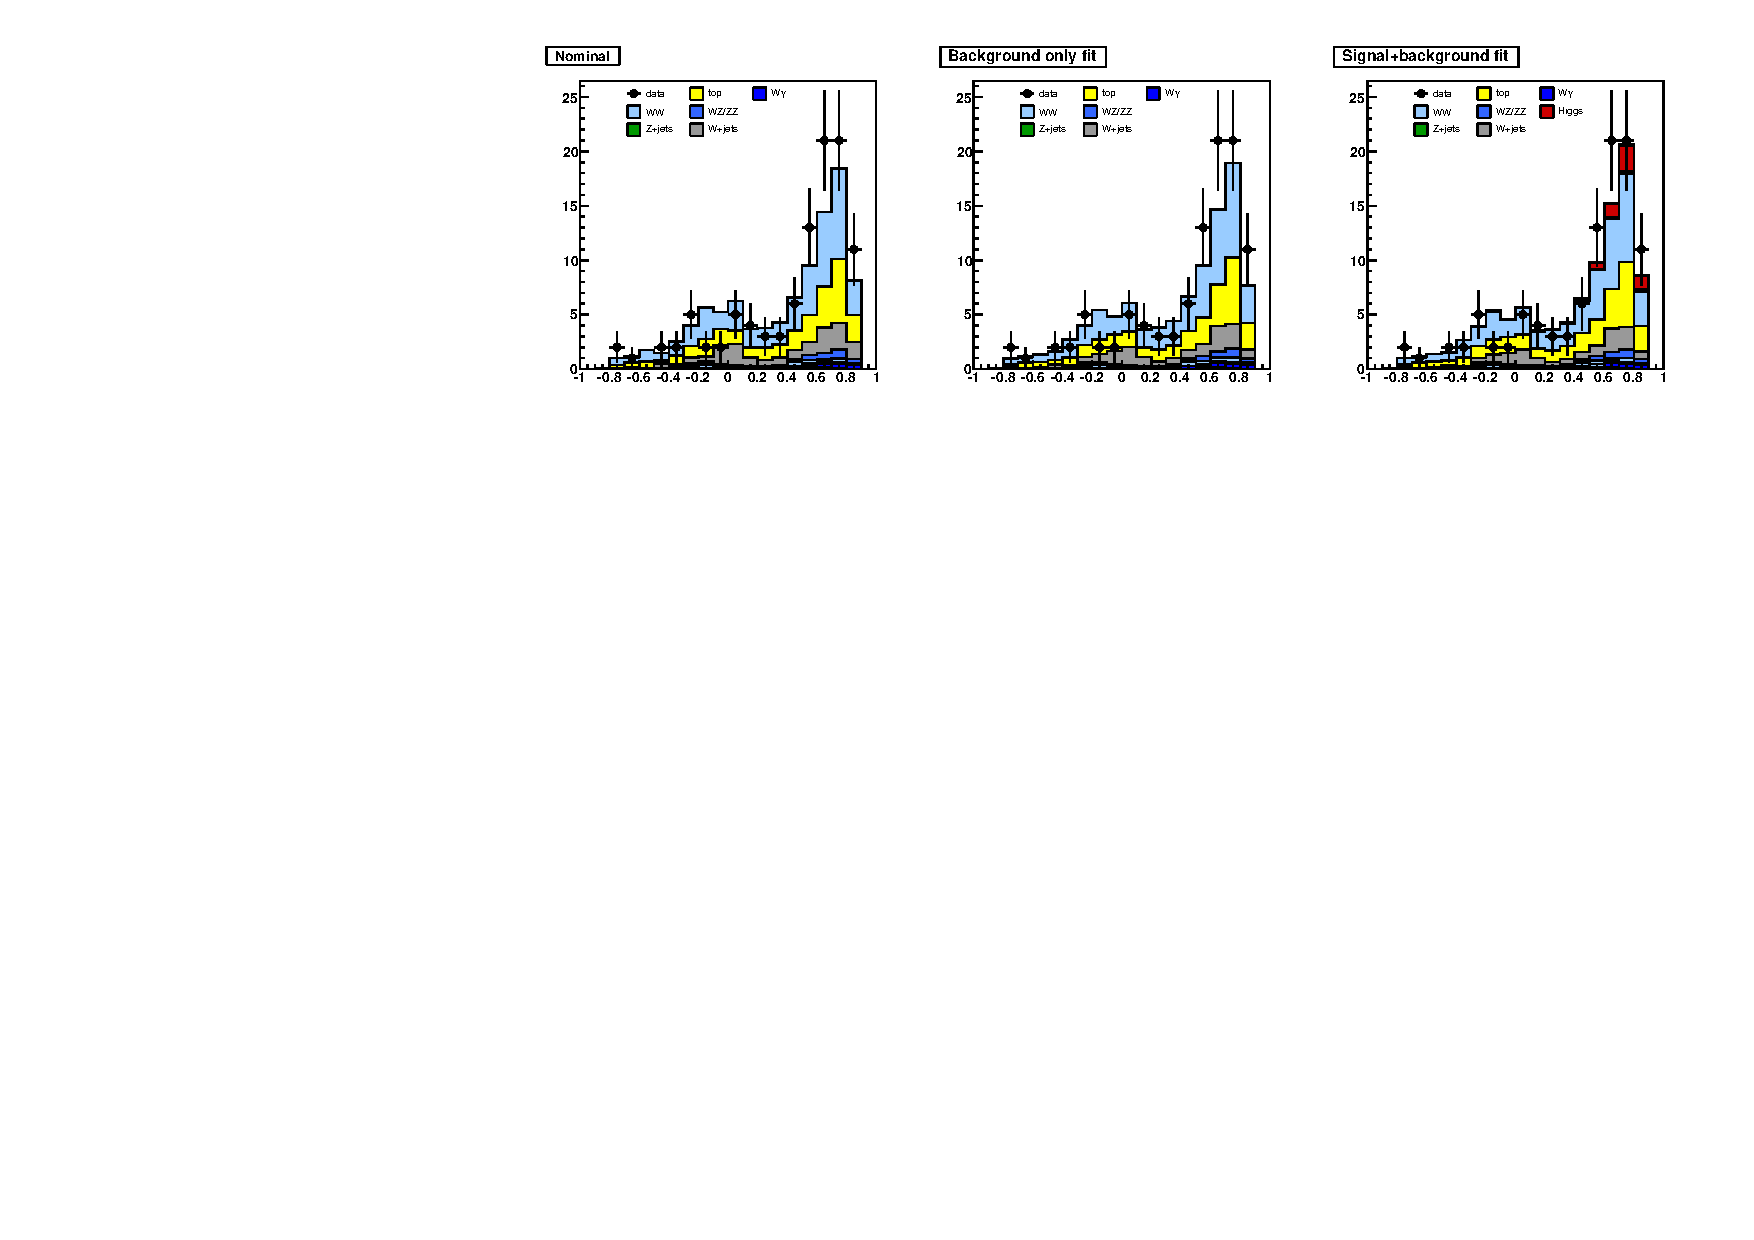
\includegraphics[width=0.9\textwidth]{figures/fits/bdt_120_n1of.pdf}}
\subfigure[$ee$/$\mu\mu$ 1-Jet]{
\centering
\label{subfig:bdt_120_n1sf}
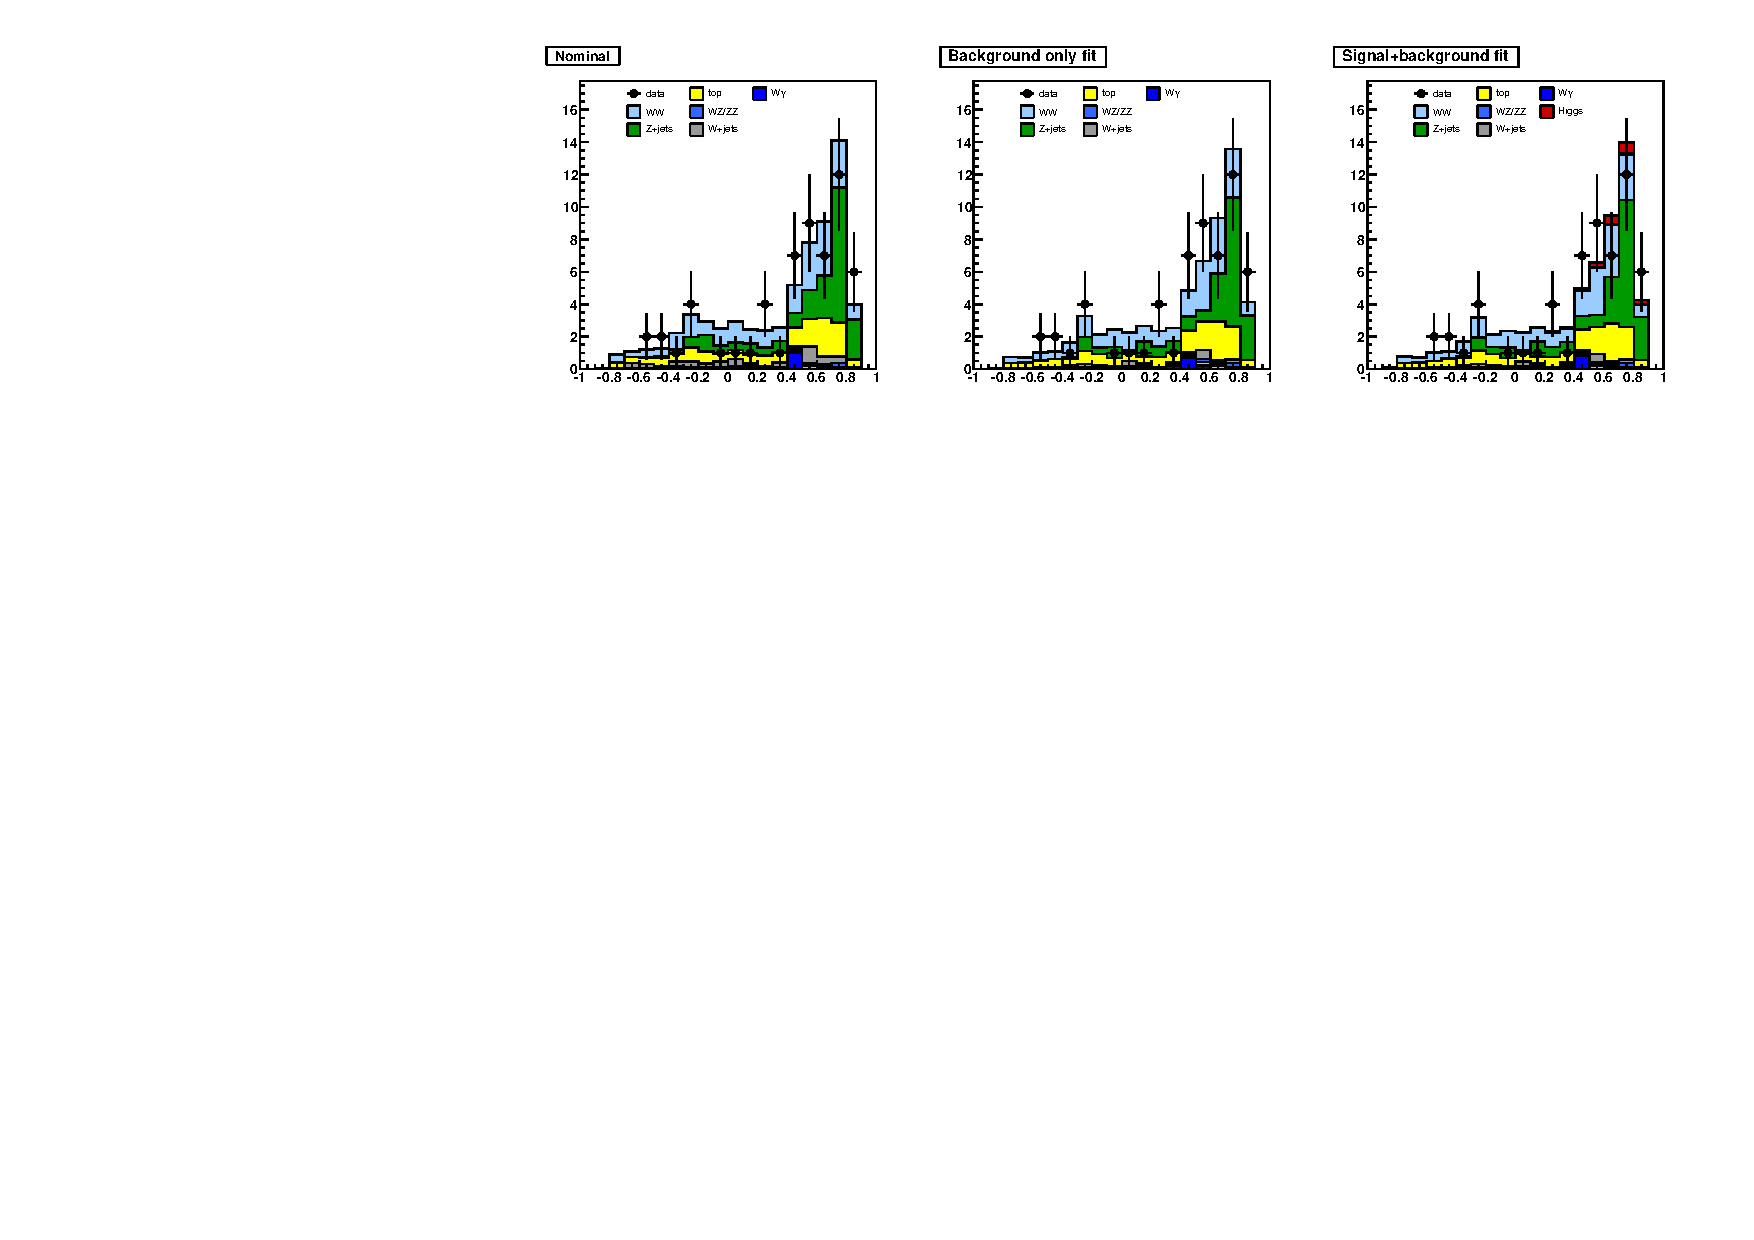
\includegraphics[width=0.9\textwidth]{figures/fits/bdt_120_n1sf.pdf}}
\caption{
MVA output distributions for Higgs 120~\GeV\ without fitting
(nominal), background fit (signal is set to zero) and
signal+background fit (signal is floating in the fit). Signal strength
for the signal+background fit is found to be 1.0 with 68\% CL range:
[0.3,1.8]}
\label{fig:fit_120}
\end{figure}

\begin{figure}[!hbtp]
\centering
\subfigure[$e\mu$ 0-Jet]{
\centering
\label{subfig:c3_130_n0of}
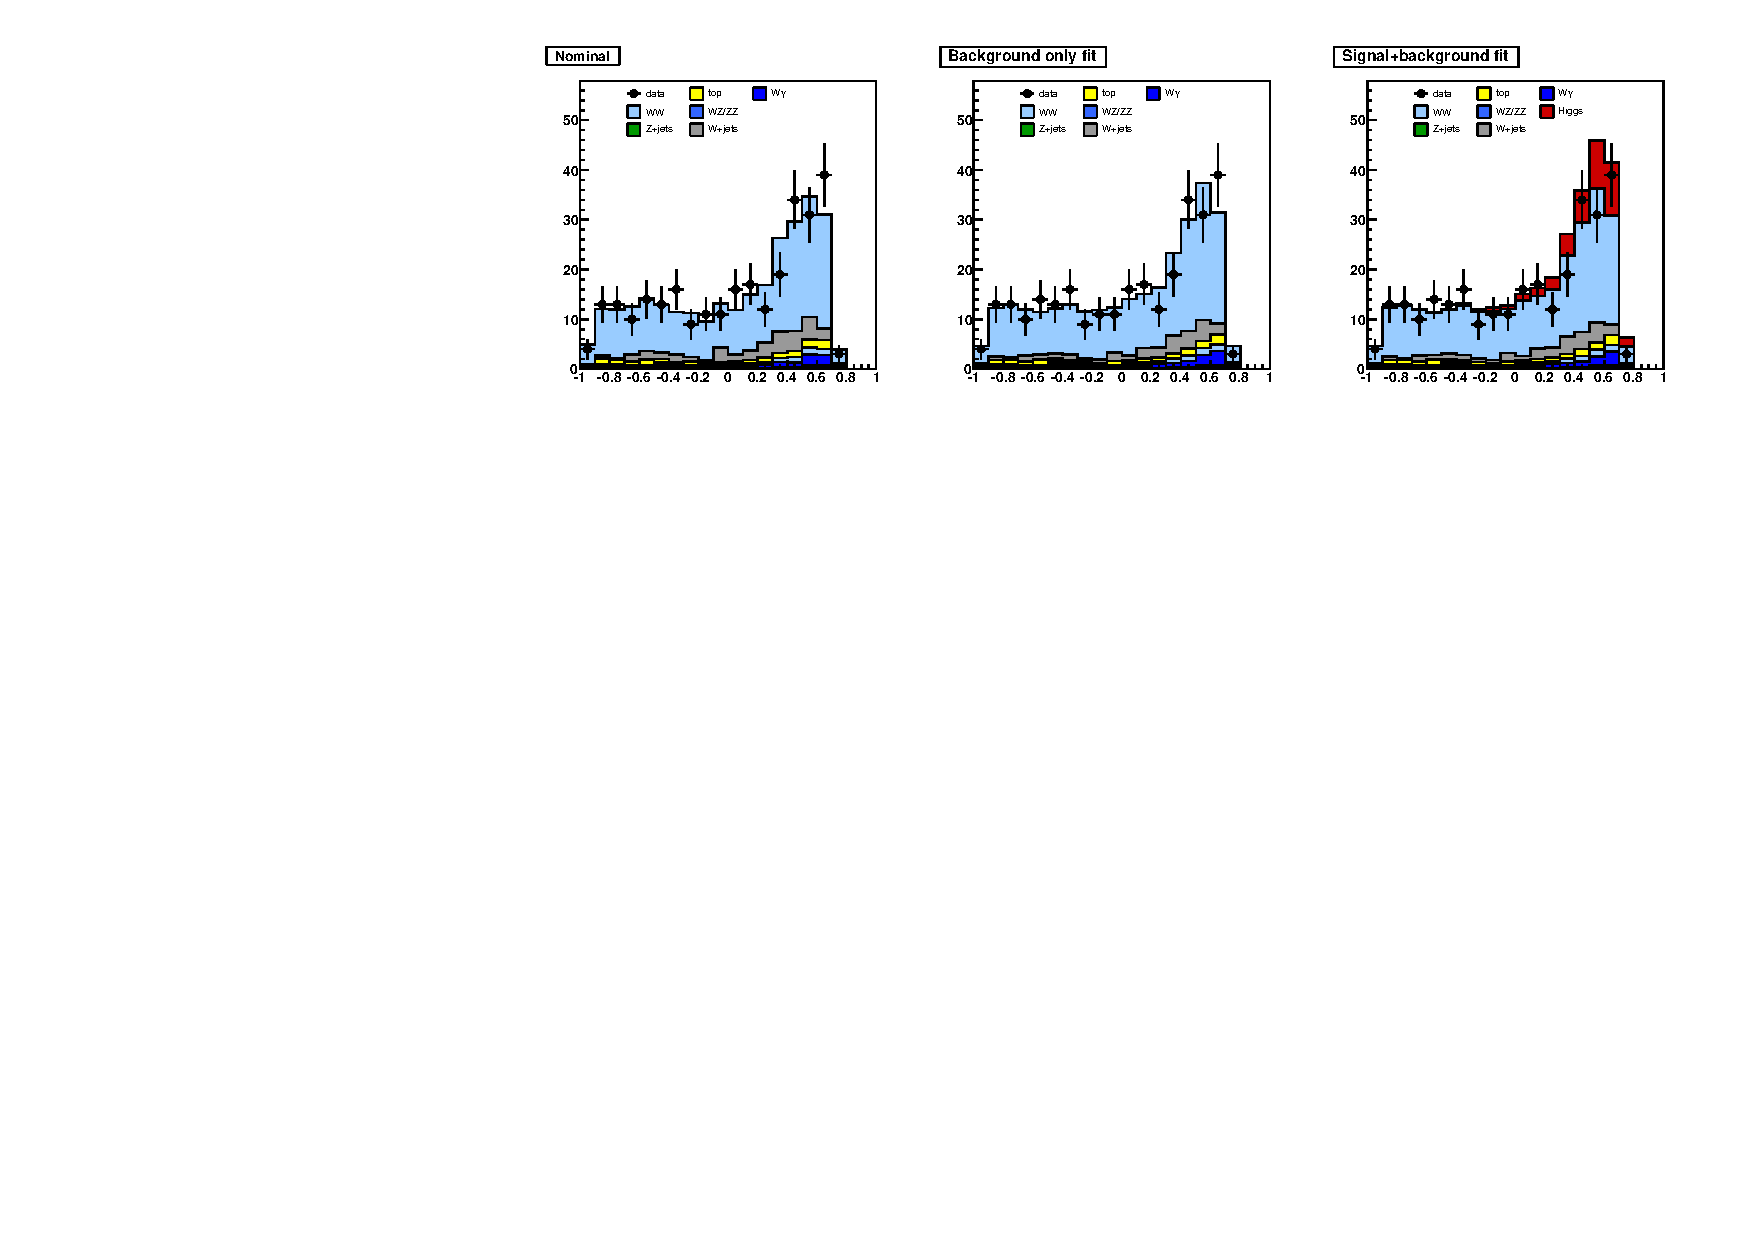
\includegraphics[width=0.9\textwidth]{figures/fits/bdt_130_n0of.pdf}}\\
\subfigure[$ee$/$\mu\mu$ 0-Jet]{
\centering
\label{subfig:bdt_130_n0sf}
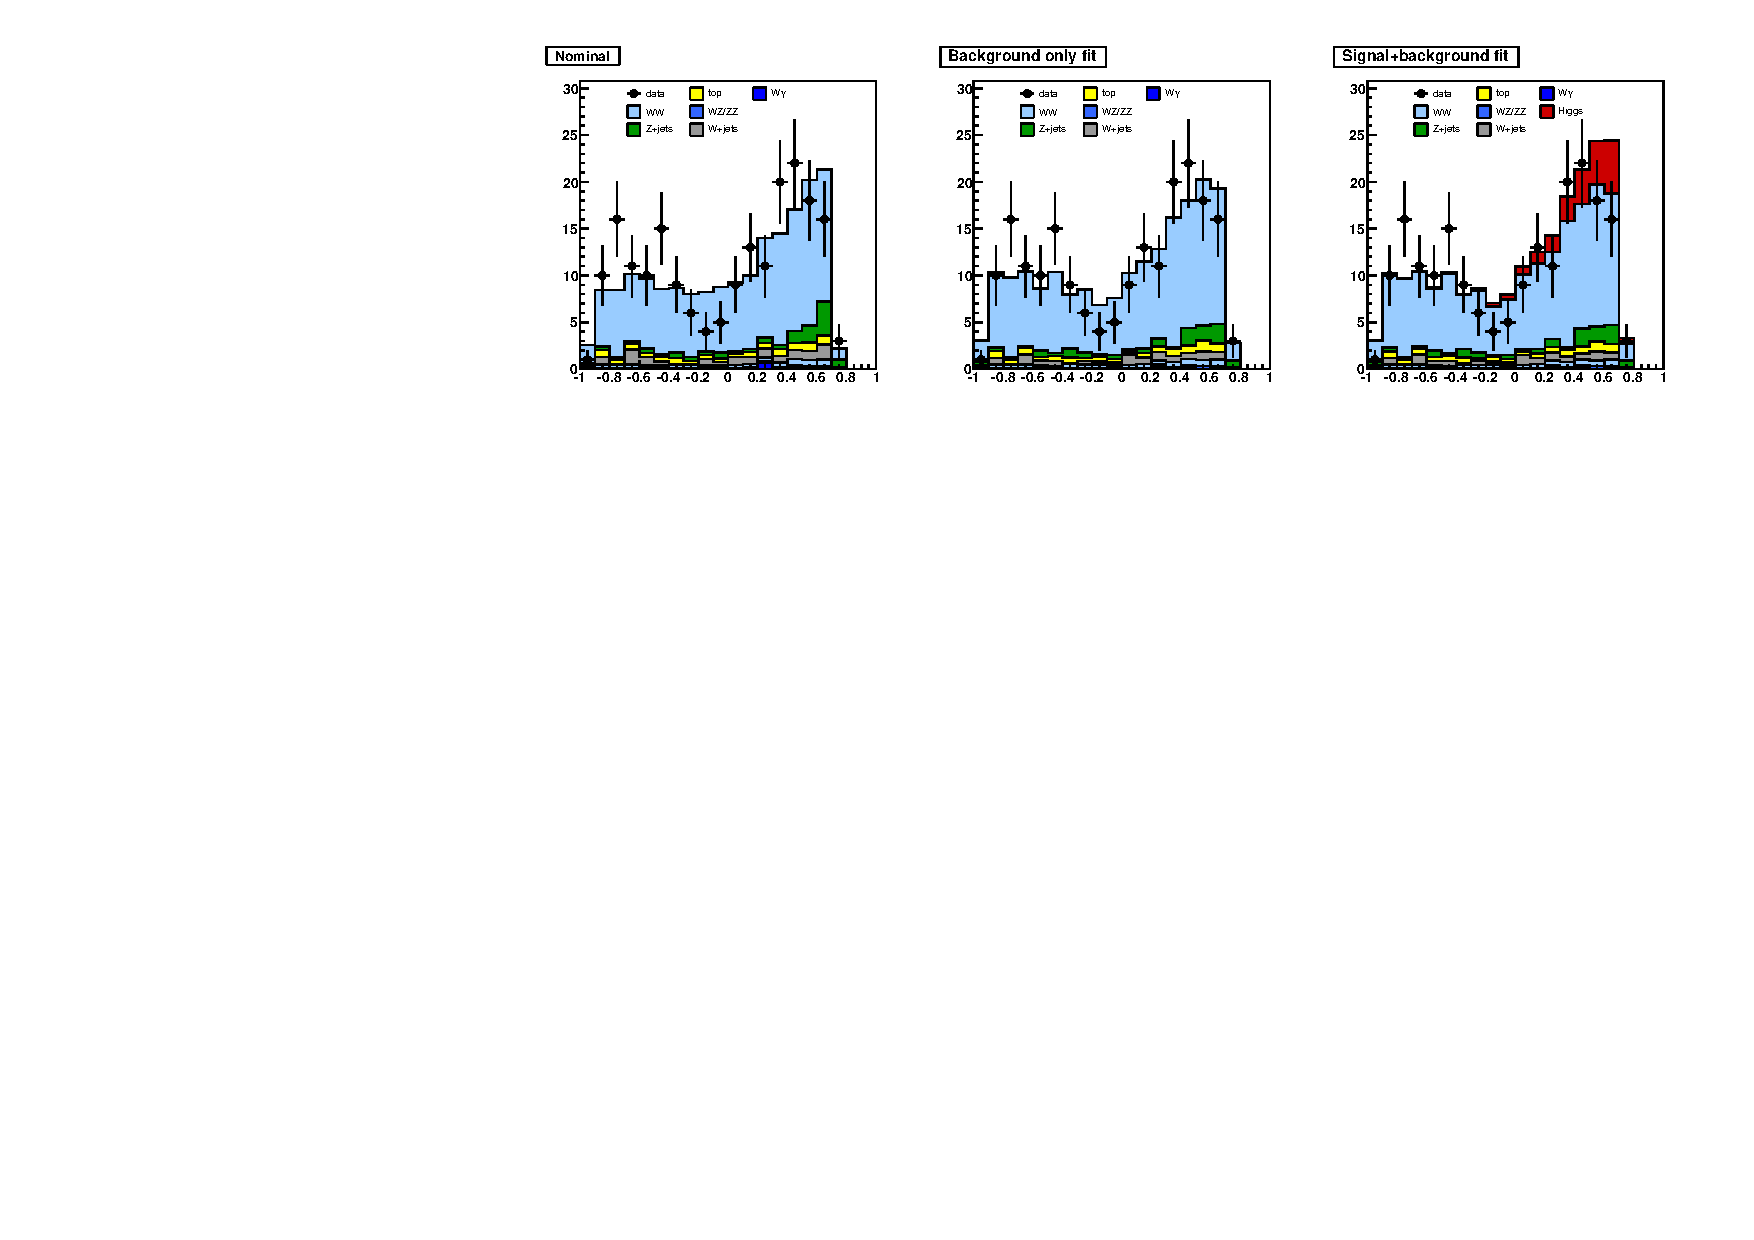
\includegraphics[width=0.9\textwidth]{figures/fits/bdt_130_n0sf.pdf}}
\subfigure[$e\mu$ 1-Jet]{
\centering
\label{subfig:bdt_130_n1of}
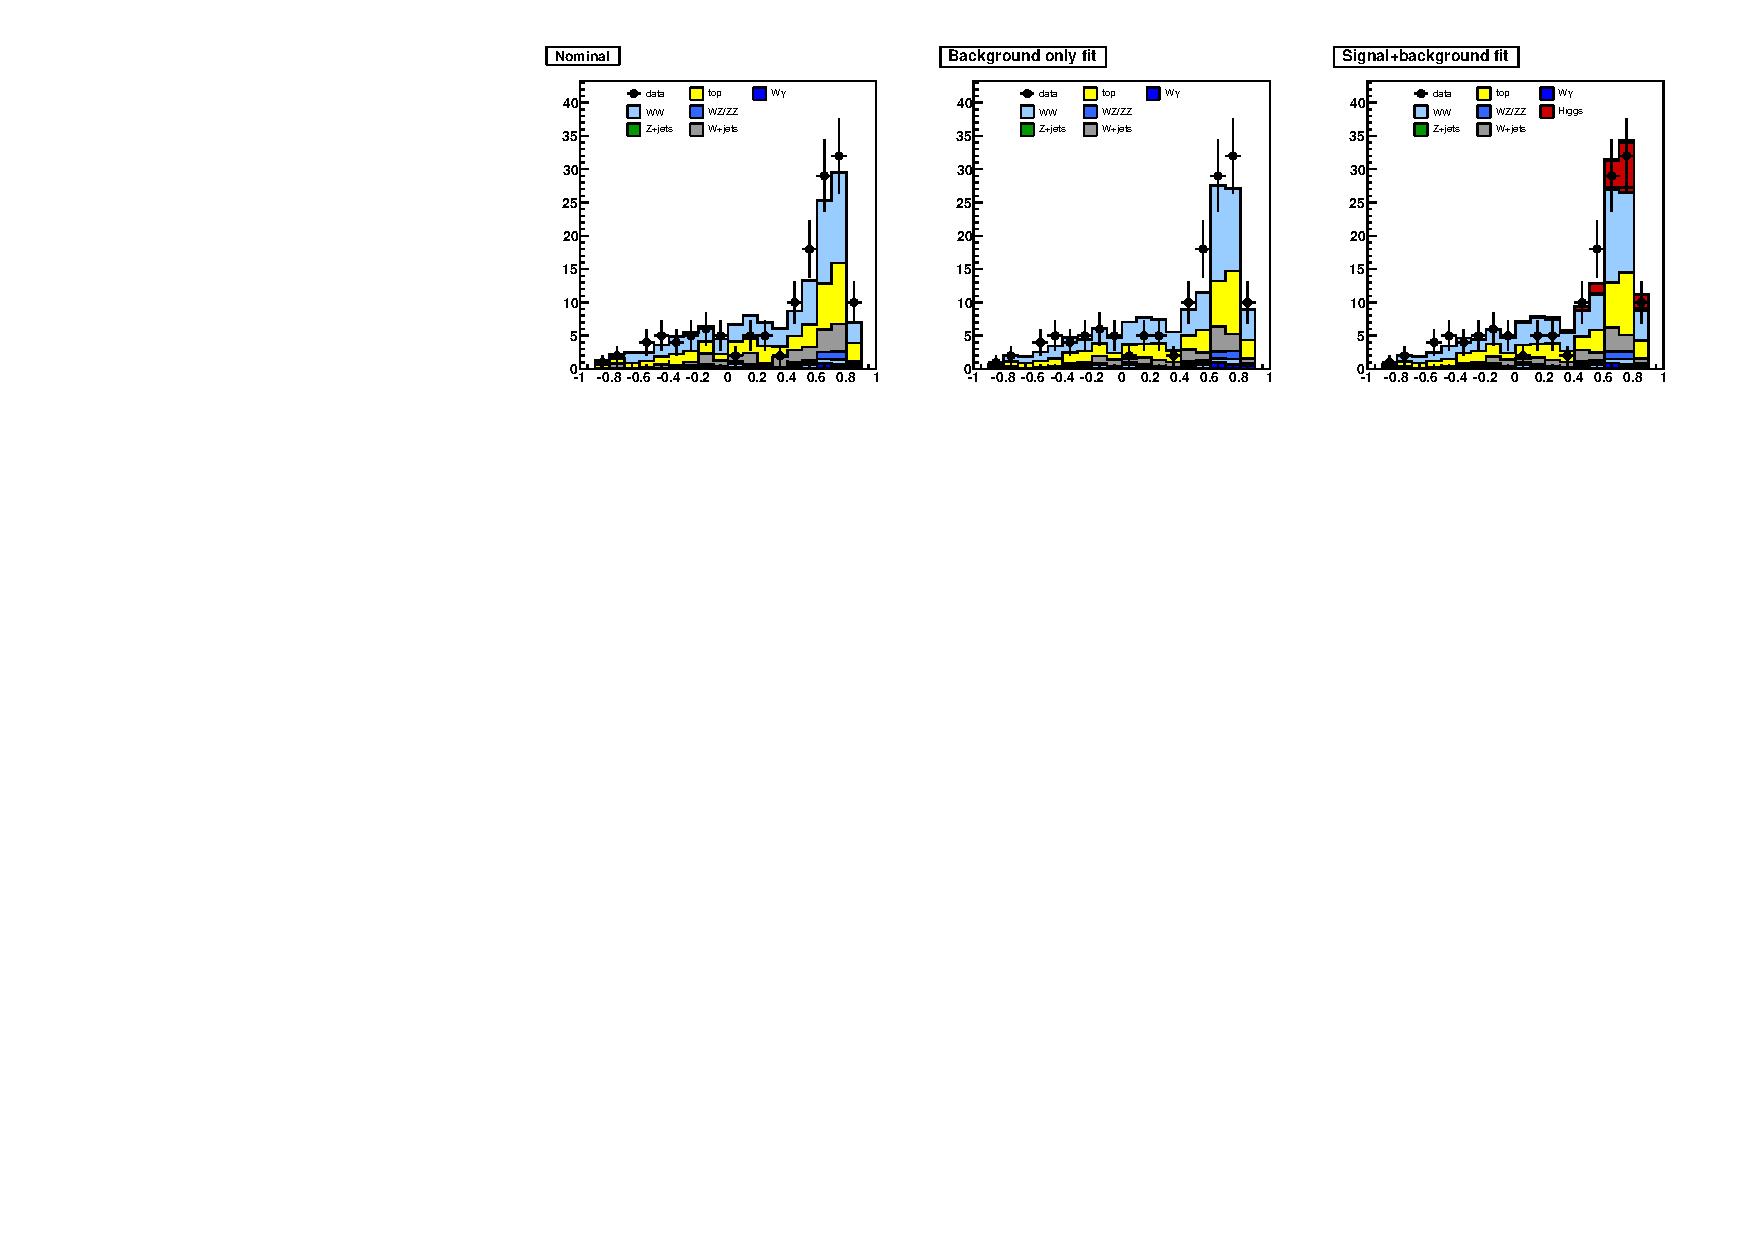
\includegraphics[width=0.9\textwidth]{figures/fits/bdt_130_n1of.pdf}}
\subfigure[$ee$/$\mu\mu$ 1-Jet]{
\centering
\label{subfig:bdt_130_n1sf}
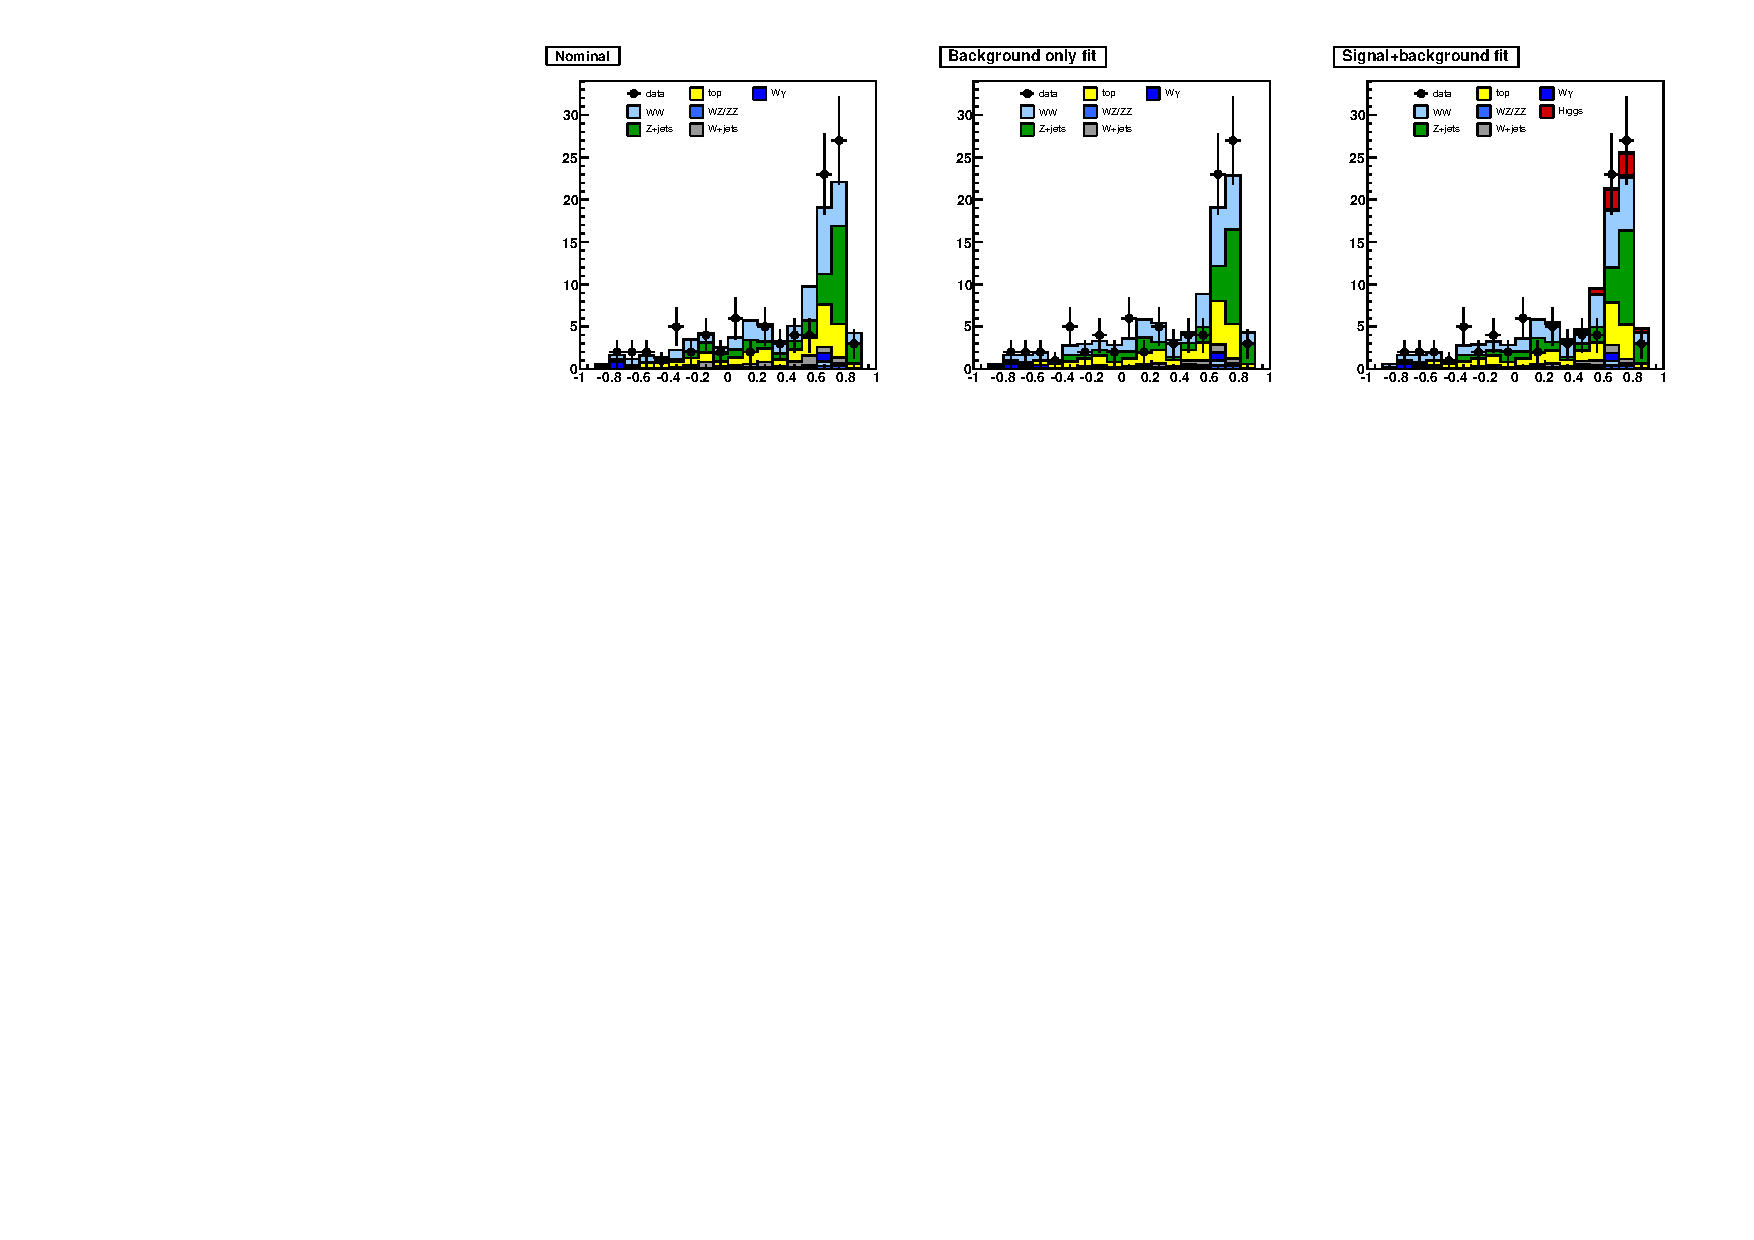
\includegraphics[width=0.9\textwidth]{figures/fits/bdt_130_n1sf.pdf}}
\caption{
MVA output distributions for Higgs 130~\GeV\ without fitting
(nominal), background fit (signal is set to zero) and
signal+background fit (signal is floating in the fit). Signal strength
for the signal+background fit is found to be 0.2 with 68\% CL range:
[-0.2,0.6]  }
\label{fig:fit_130}
\end{figure}

\begin{figure}[!hbtp]
\centering
\subfigure[$e\mu$ 0-Jet]{
\centering
\label{subfig:c3_350_n0of}
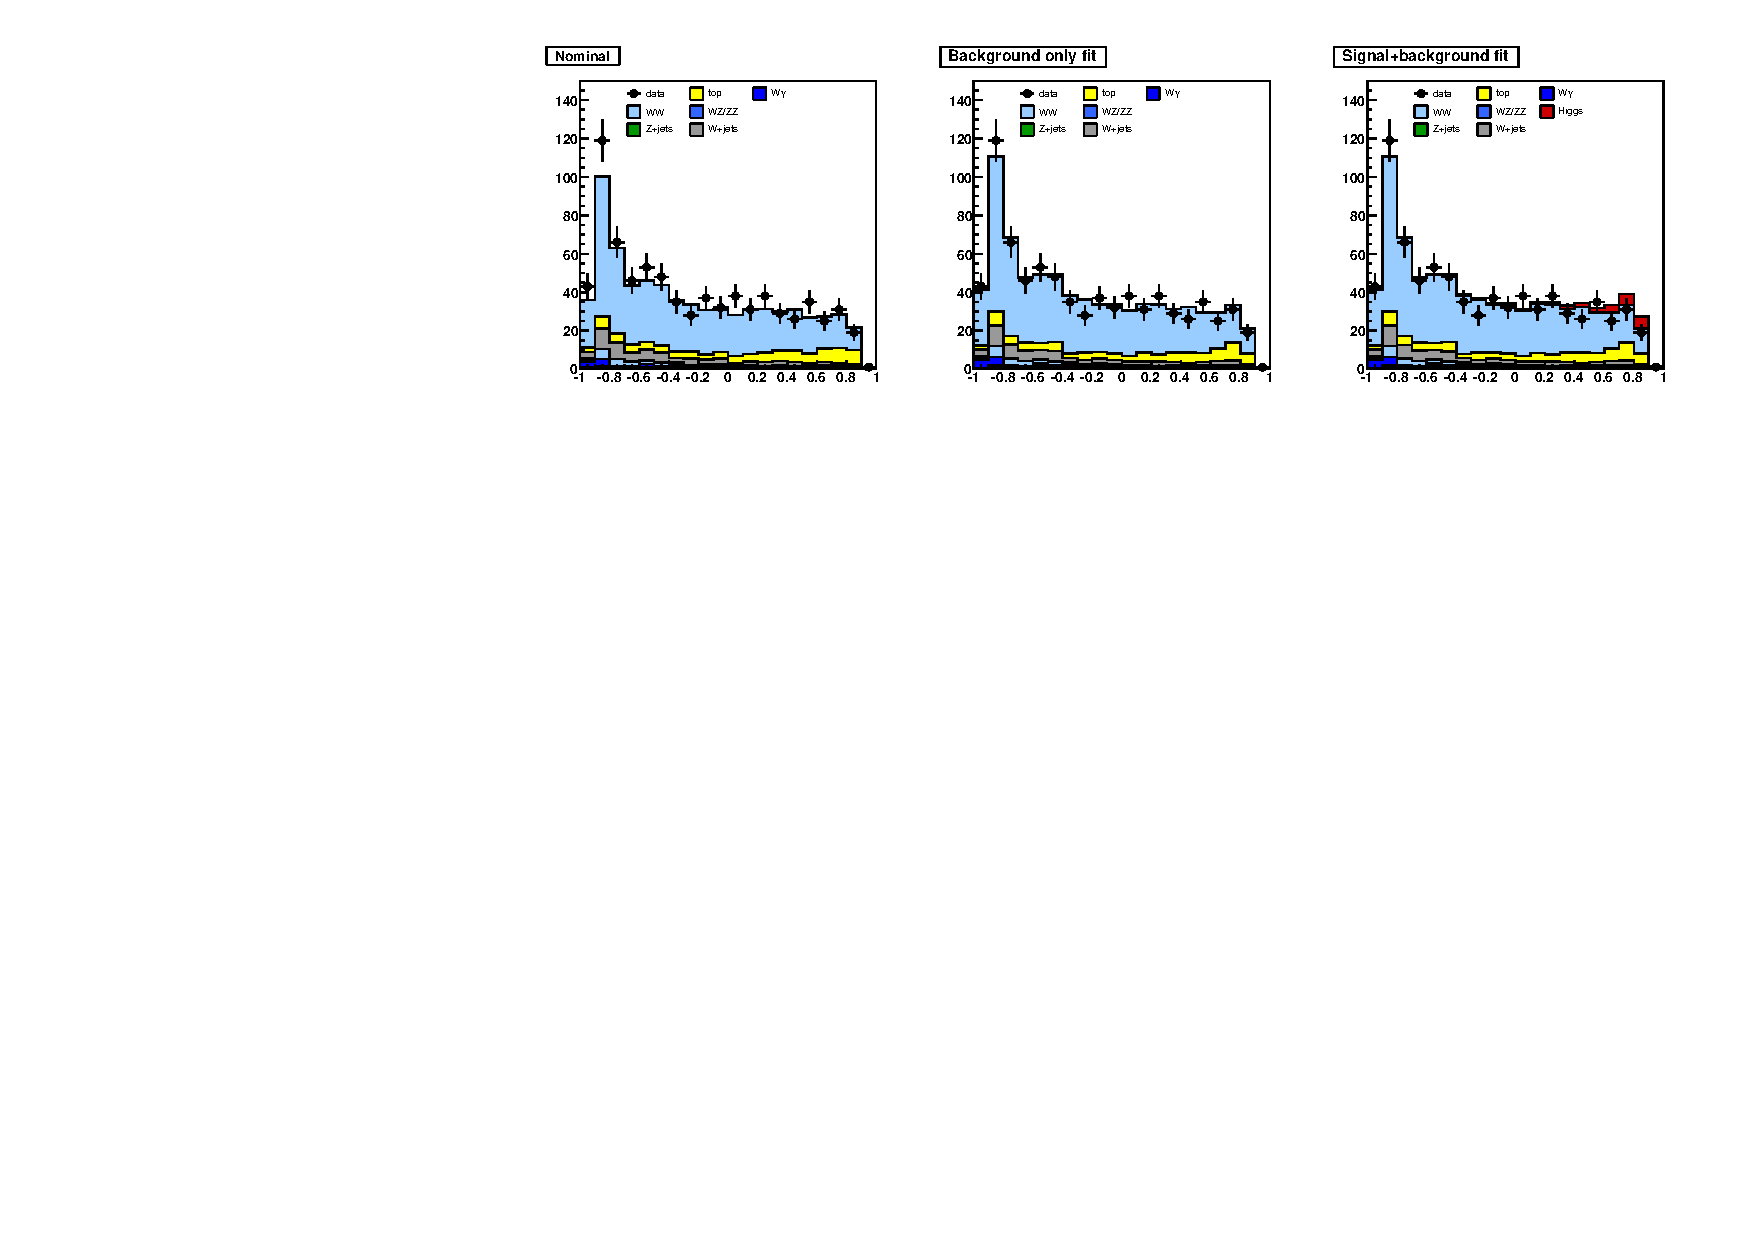
\includegraphics[width=0.9\textwidth]{figures/fits/bdt_350_n0of.pdf}}\\
\subfigure[$ee$/$\mu\mu$ 0-Jet]{
\centering
\label{subfig:bdt_350_n0sf}
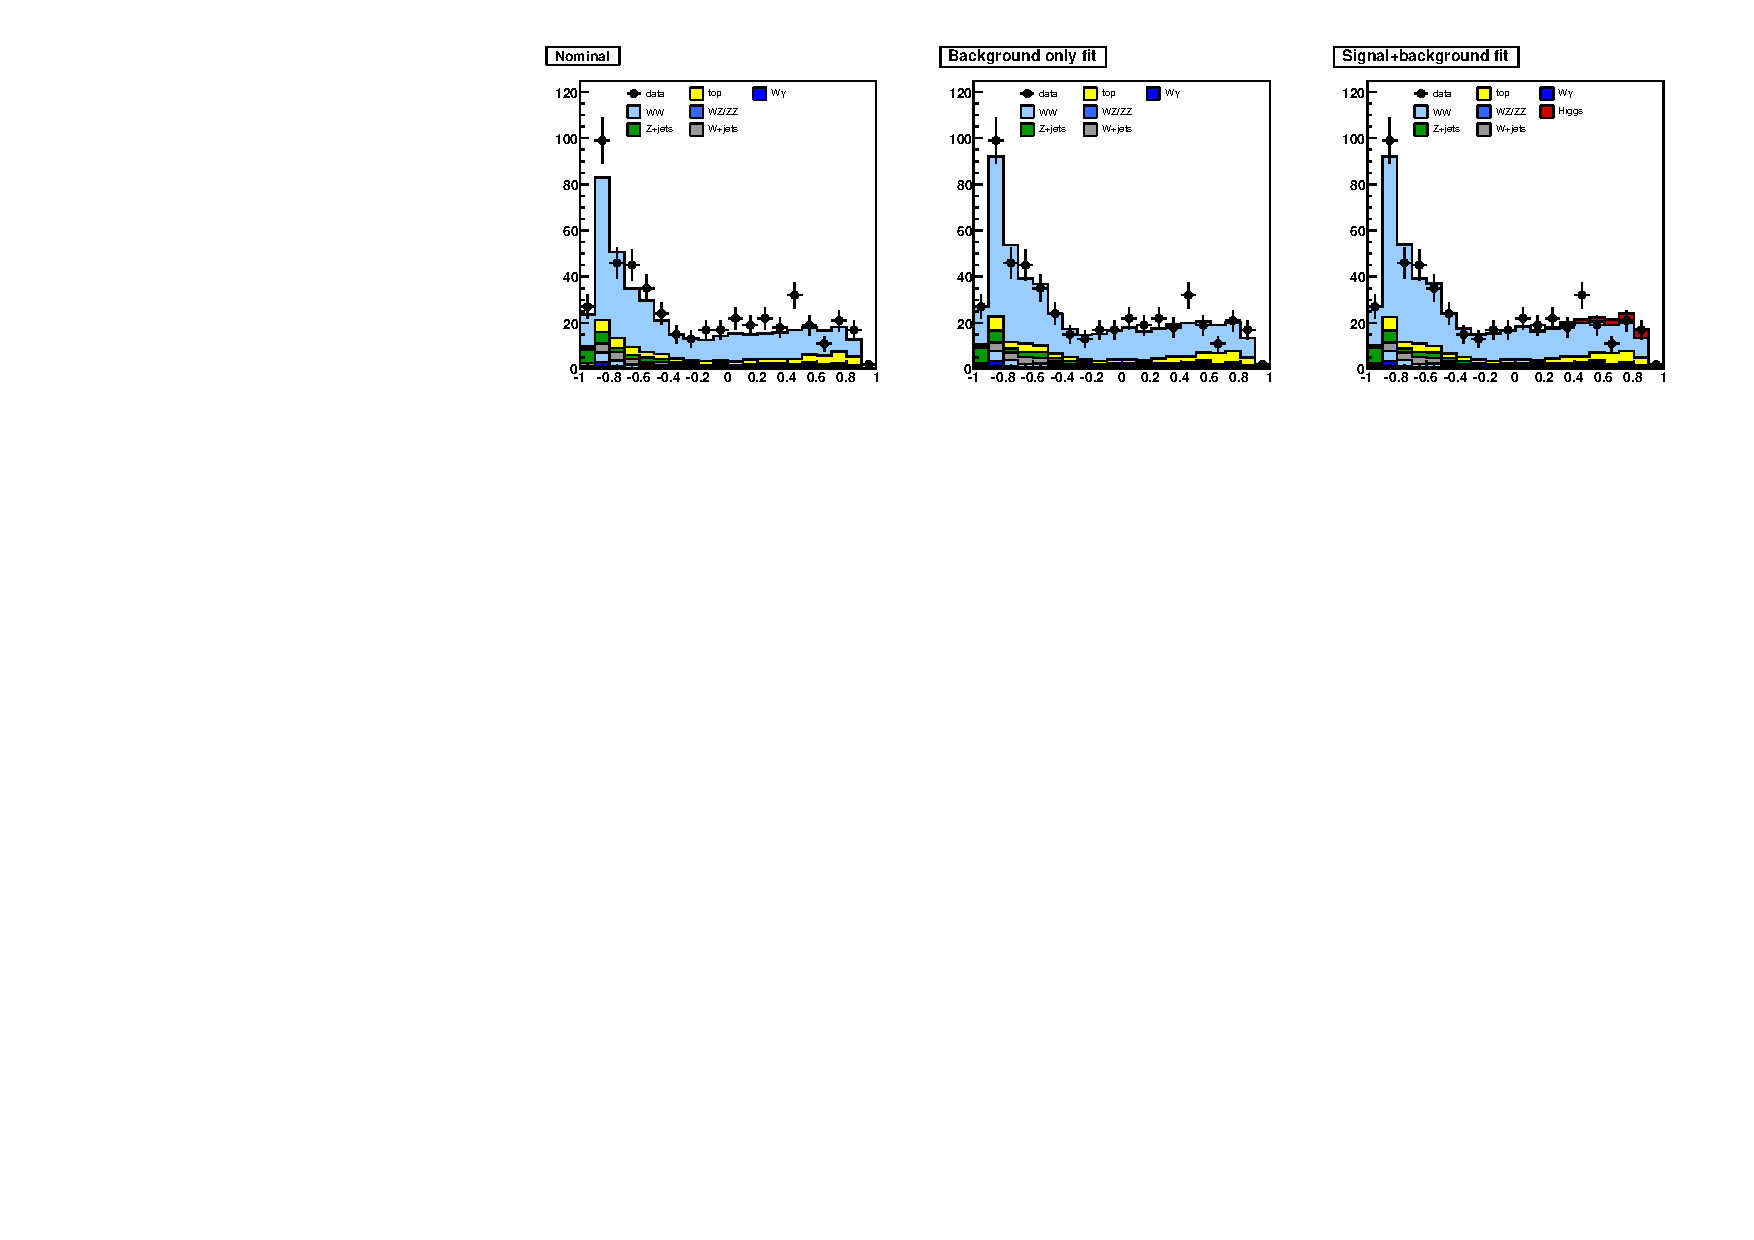
\includegraphics[width=0.9\textwidth]{figures/fits/bdt_350_n0sf.pdf}}
\subfigure[$e\mu$ 1-Jet]{
\centering
\label{subfig:bdt_350_n1of}
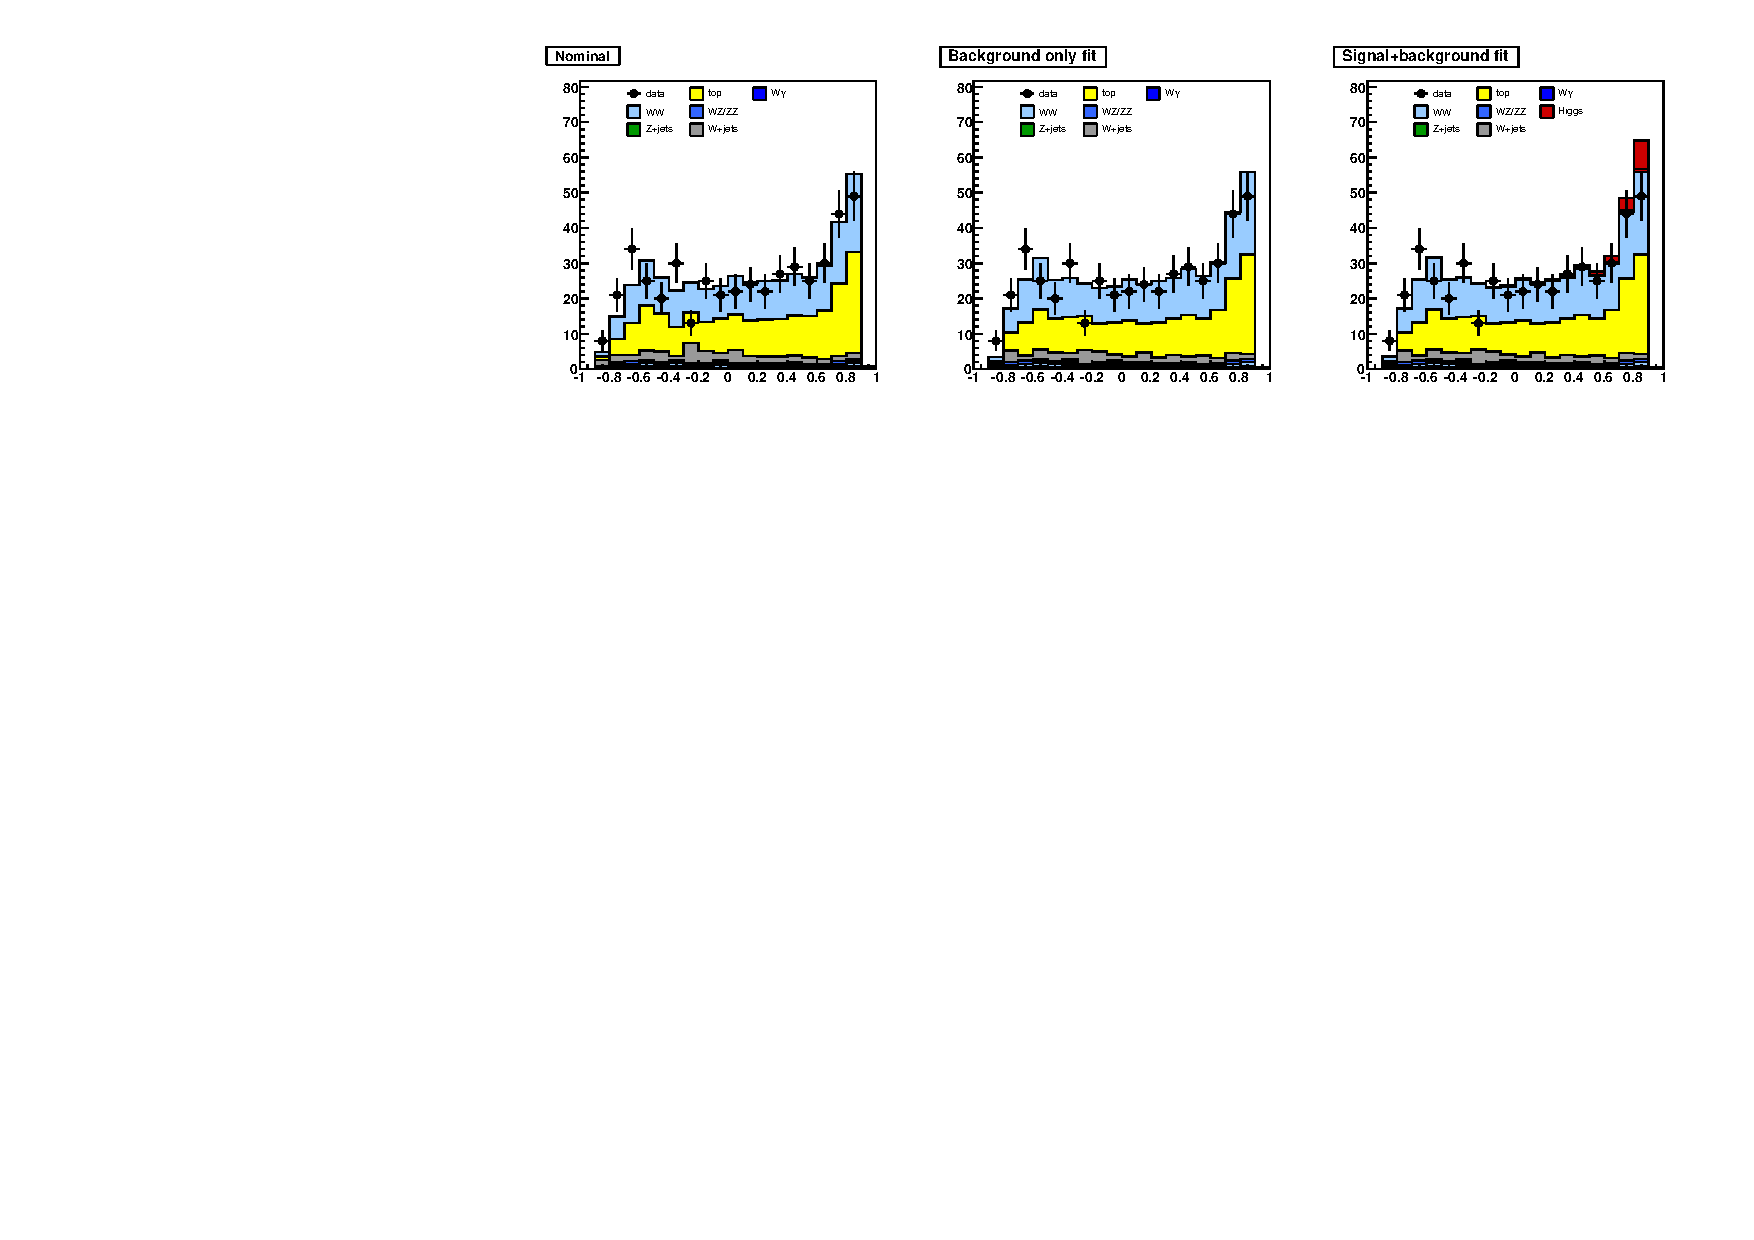
\includegraphics[width=0.9\textwidth]{figures/fits/bdt_350_n1of.pdf}}
\subfigure[$ee$/$\mu\mu$ 1-Jet]{
\centering
\label{subfig:bdt_350_n1sf}
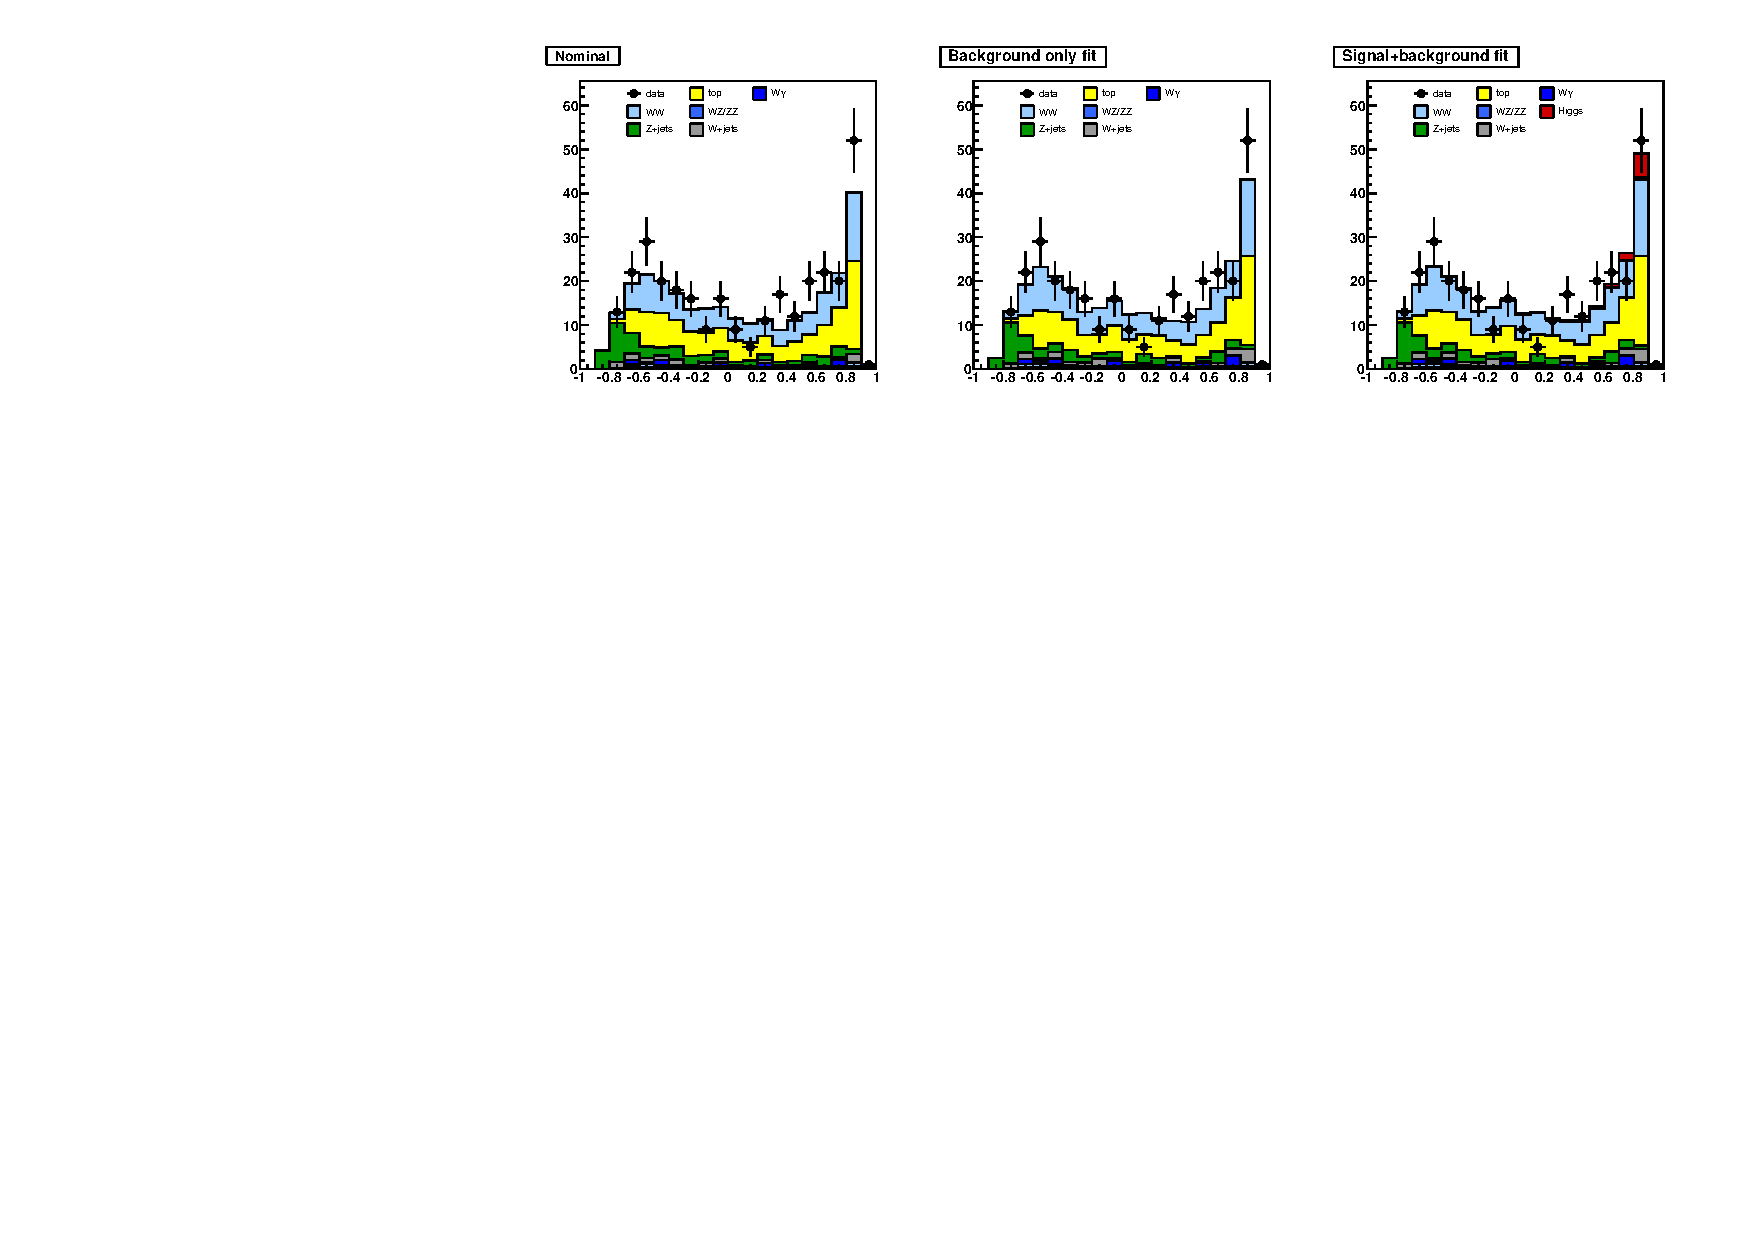
\includegraphics[width=0.9\textwidth]{figures/fits/bdt_350_n1sf.pdf}}
\caption{
MVA output distributions for Higgs 350~\GeV\ without fitting
(nominal), background fit (signal is set to zero) and
signal+background fit (signal is floating in the fit). Signal strength
for the signal+background fit is found to be 0.0 with 68\% CL range:
[0.0,0.4]  }
\label{fig:fit_350}
\end{figure}

\begin{figure}[!hbtp]
\centering
\subfigure[$e\mu$ 0-Jet]{
\centering
\label{subfig:c3_400_n0of}
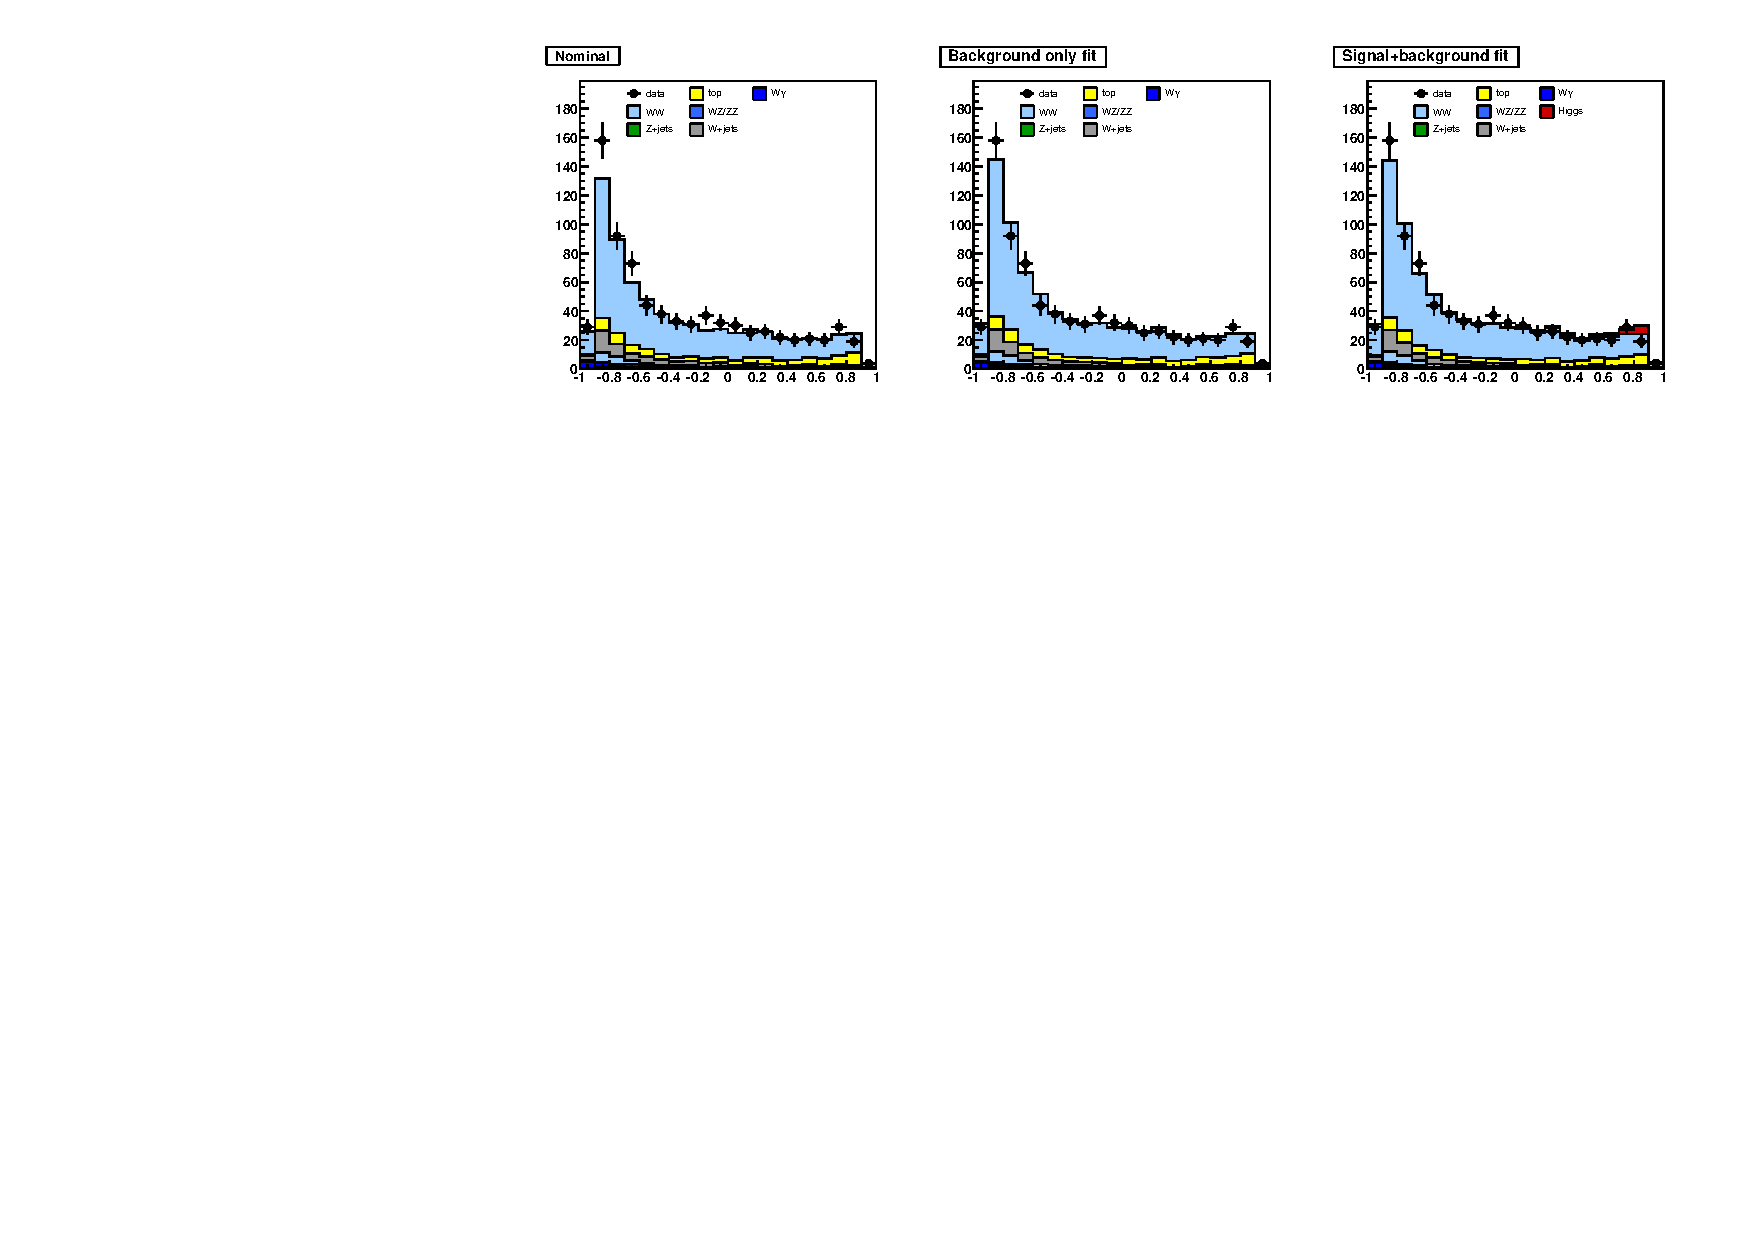
\includegraphics[width=0.9\textwidth]{figures/fits/bdt_400_n0of.pdf}}\\
\subfigure[$ee$/$\mu\mu$ 0-Jet]{
\centering
\label{subfig:bdt_400_n0sf}
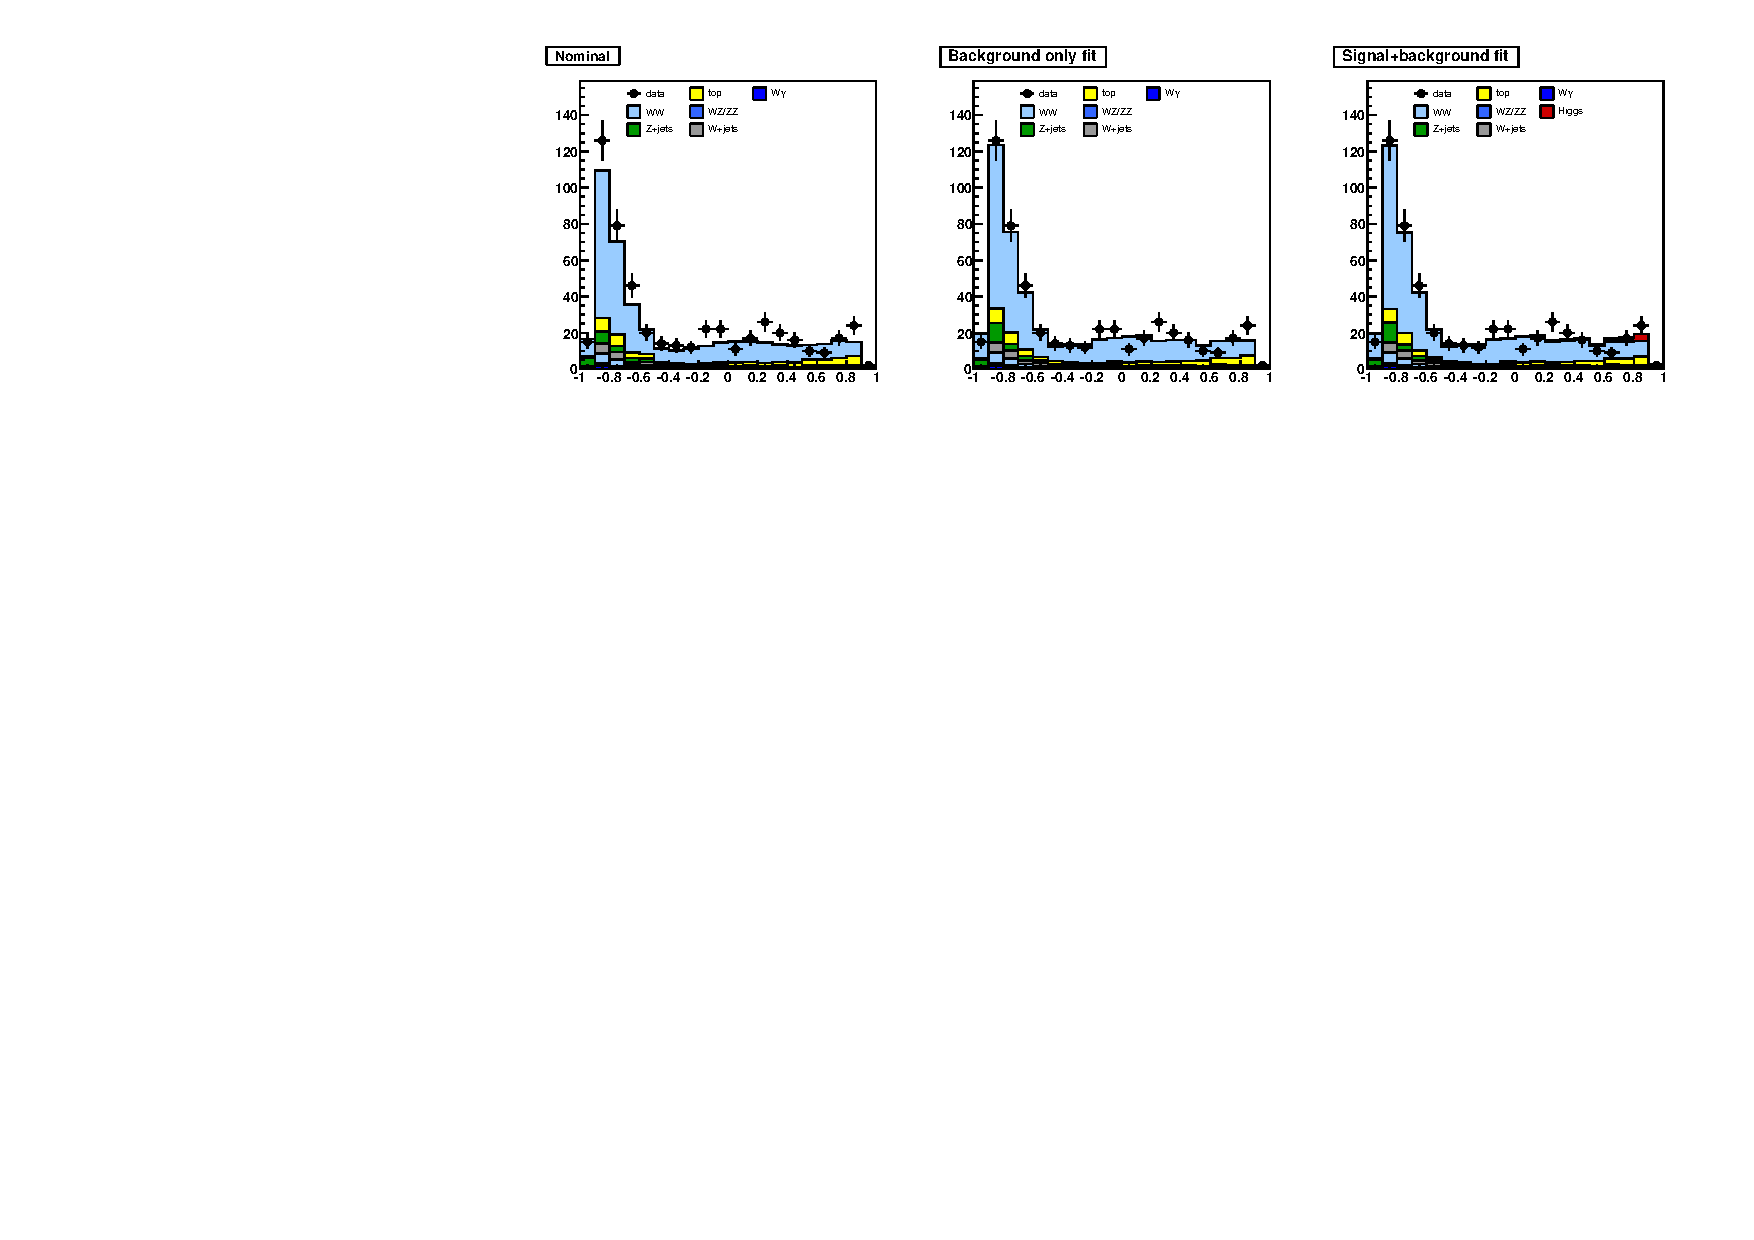
\includegraphics[width=0.9\textwidth]{figures/fits/bdt_400_n0sf.pdf}}
\subfigure[$e\mu$ 1-Jet]{
\centering
\label{subfig:bdt_400_n1of}
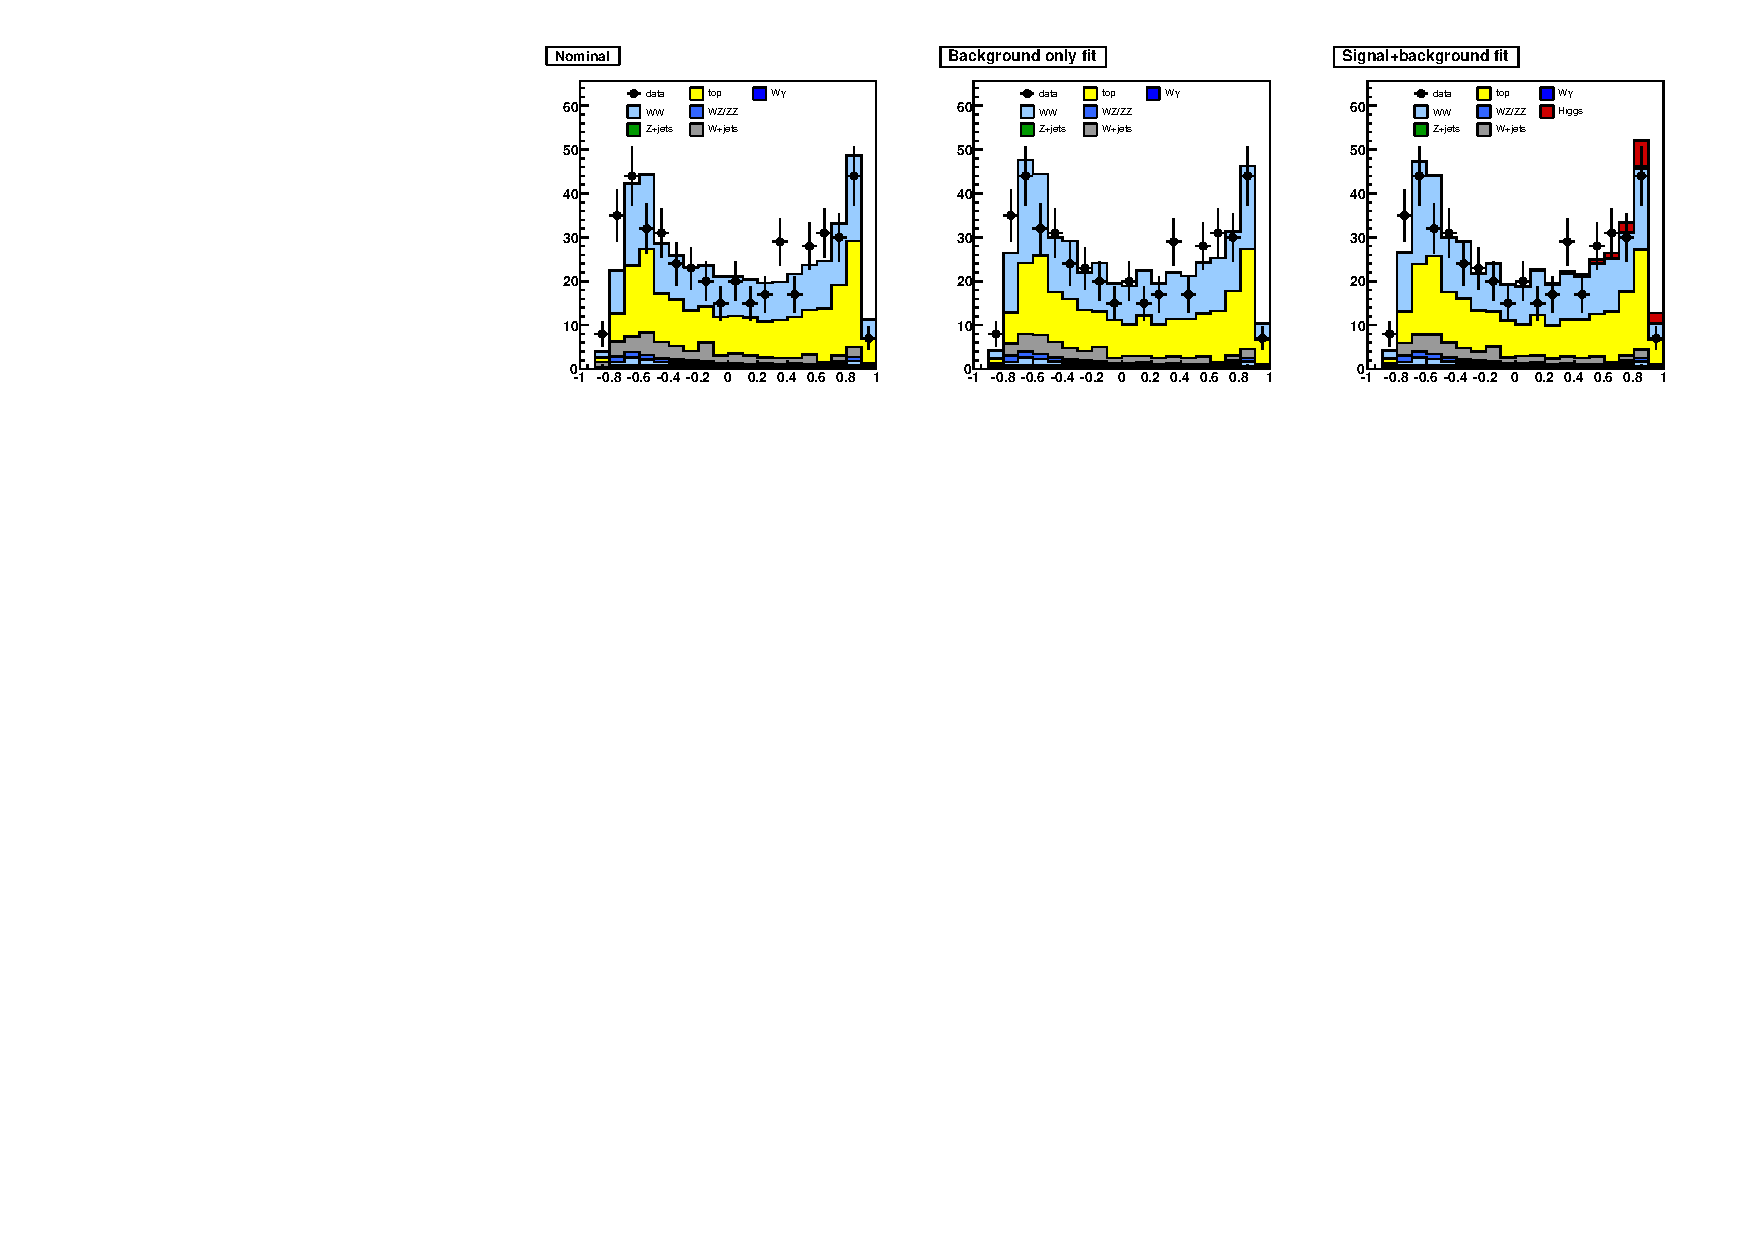
\includegraphics[width=0.9\textwidth]{figures/fits/bdt_400_n1of.pdf}}
\subfigure[$ee$/$\mu\mu$ 1-Jet]{
\centering
\label{subfig:bdt_400_n1sf}
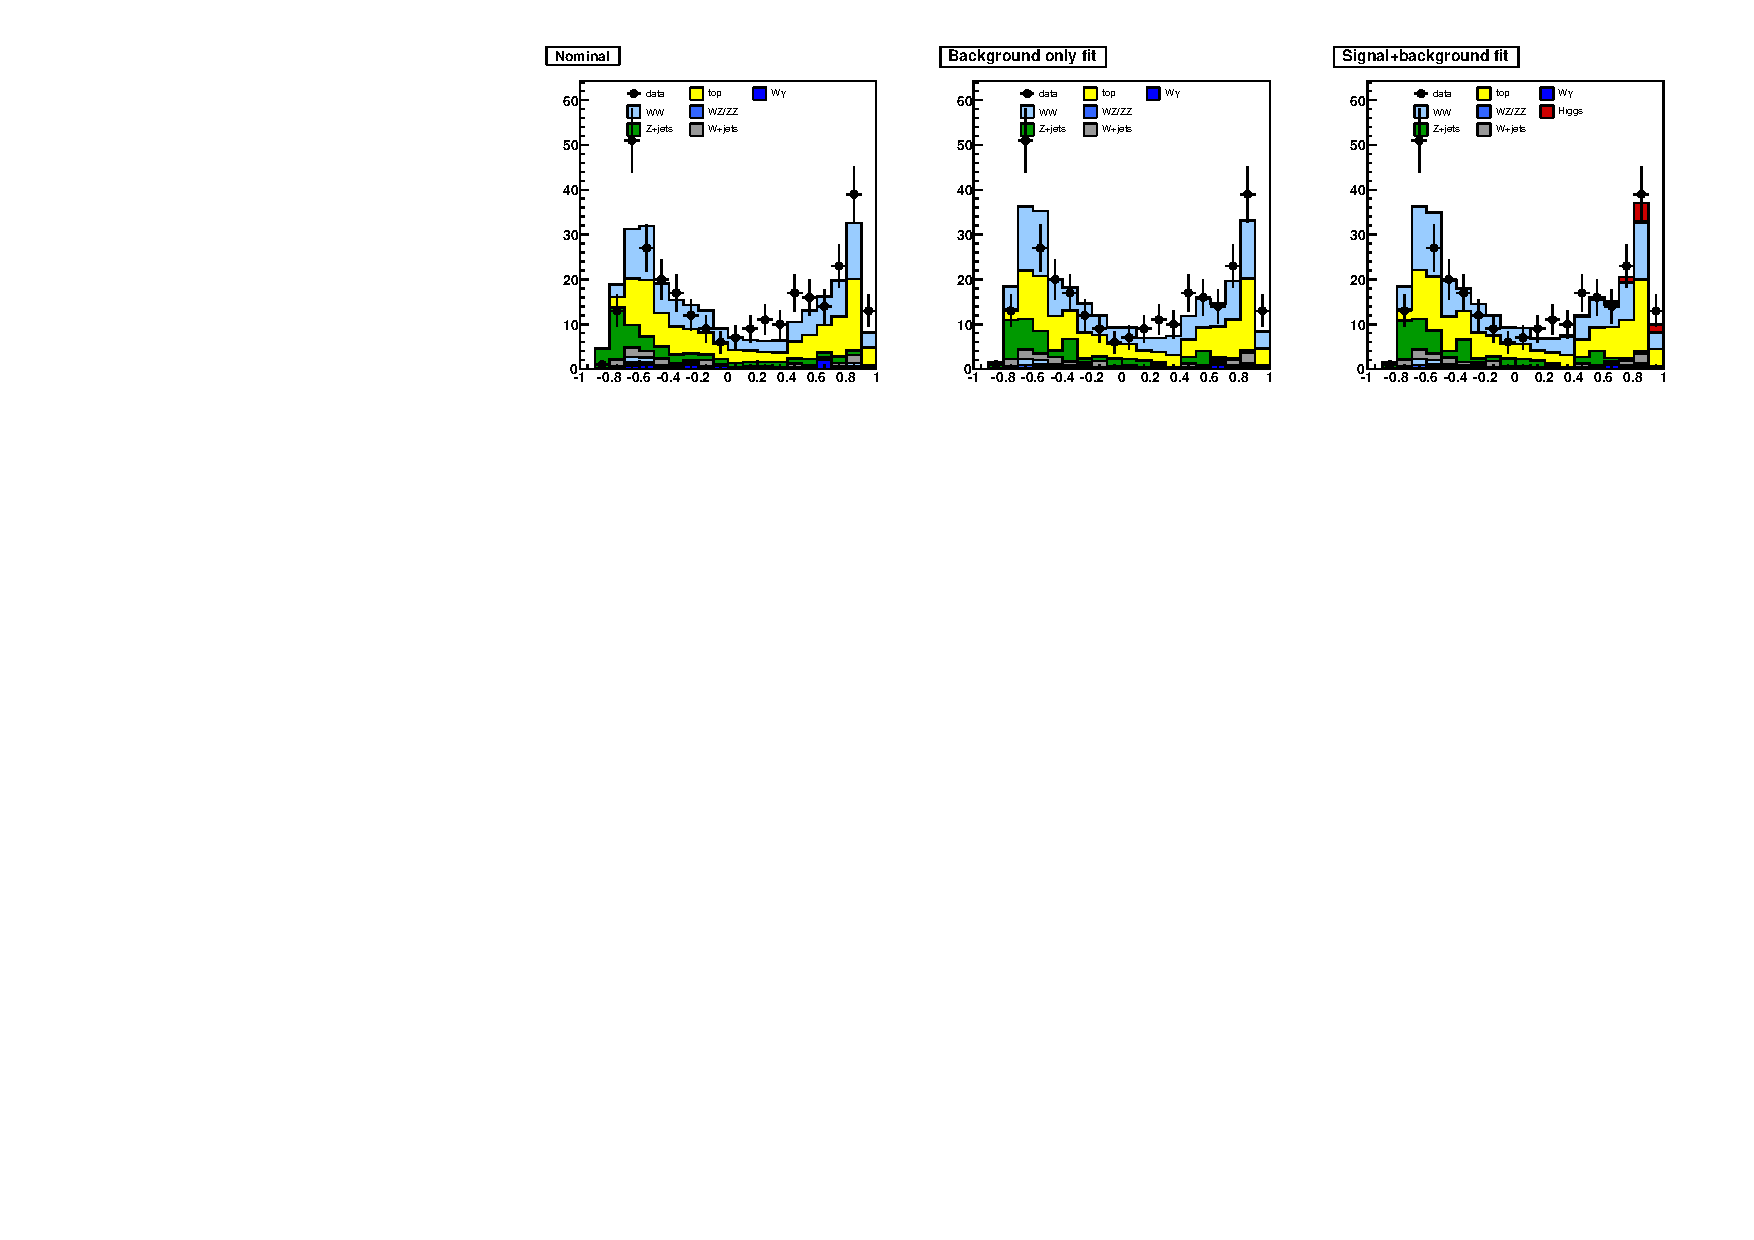
\includegraphics[width=0.9\textwidth]{figures/fits/bdt_400_n1sf.pdf}}
\caption{
MVA output distributions for Higgs 400~\GeV\ without fitting
(nominal), background fit (signal is set to zero) and
signal+background fit (signal is floating in the fit). Signal strength
for the signal+background fit is found to be 0.3 with 68\% CL range:
[-0.1,0.8] 
 }
\label{fig:fit_400}
\end{figure}

\begin{figure}[!hbtp]
\centering
\subfigure[$e\mu$ 0-Jet]{
\centering
\label{subfig:bdt2_115_n0of}
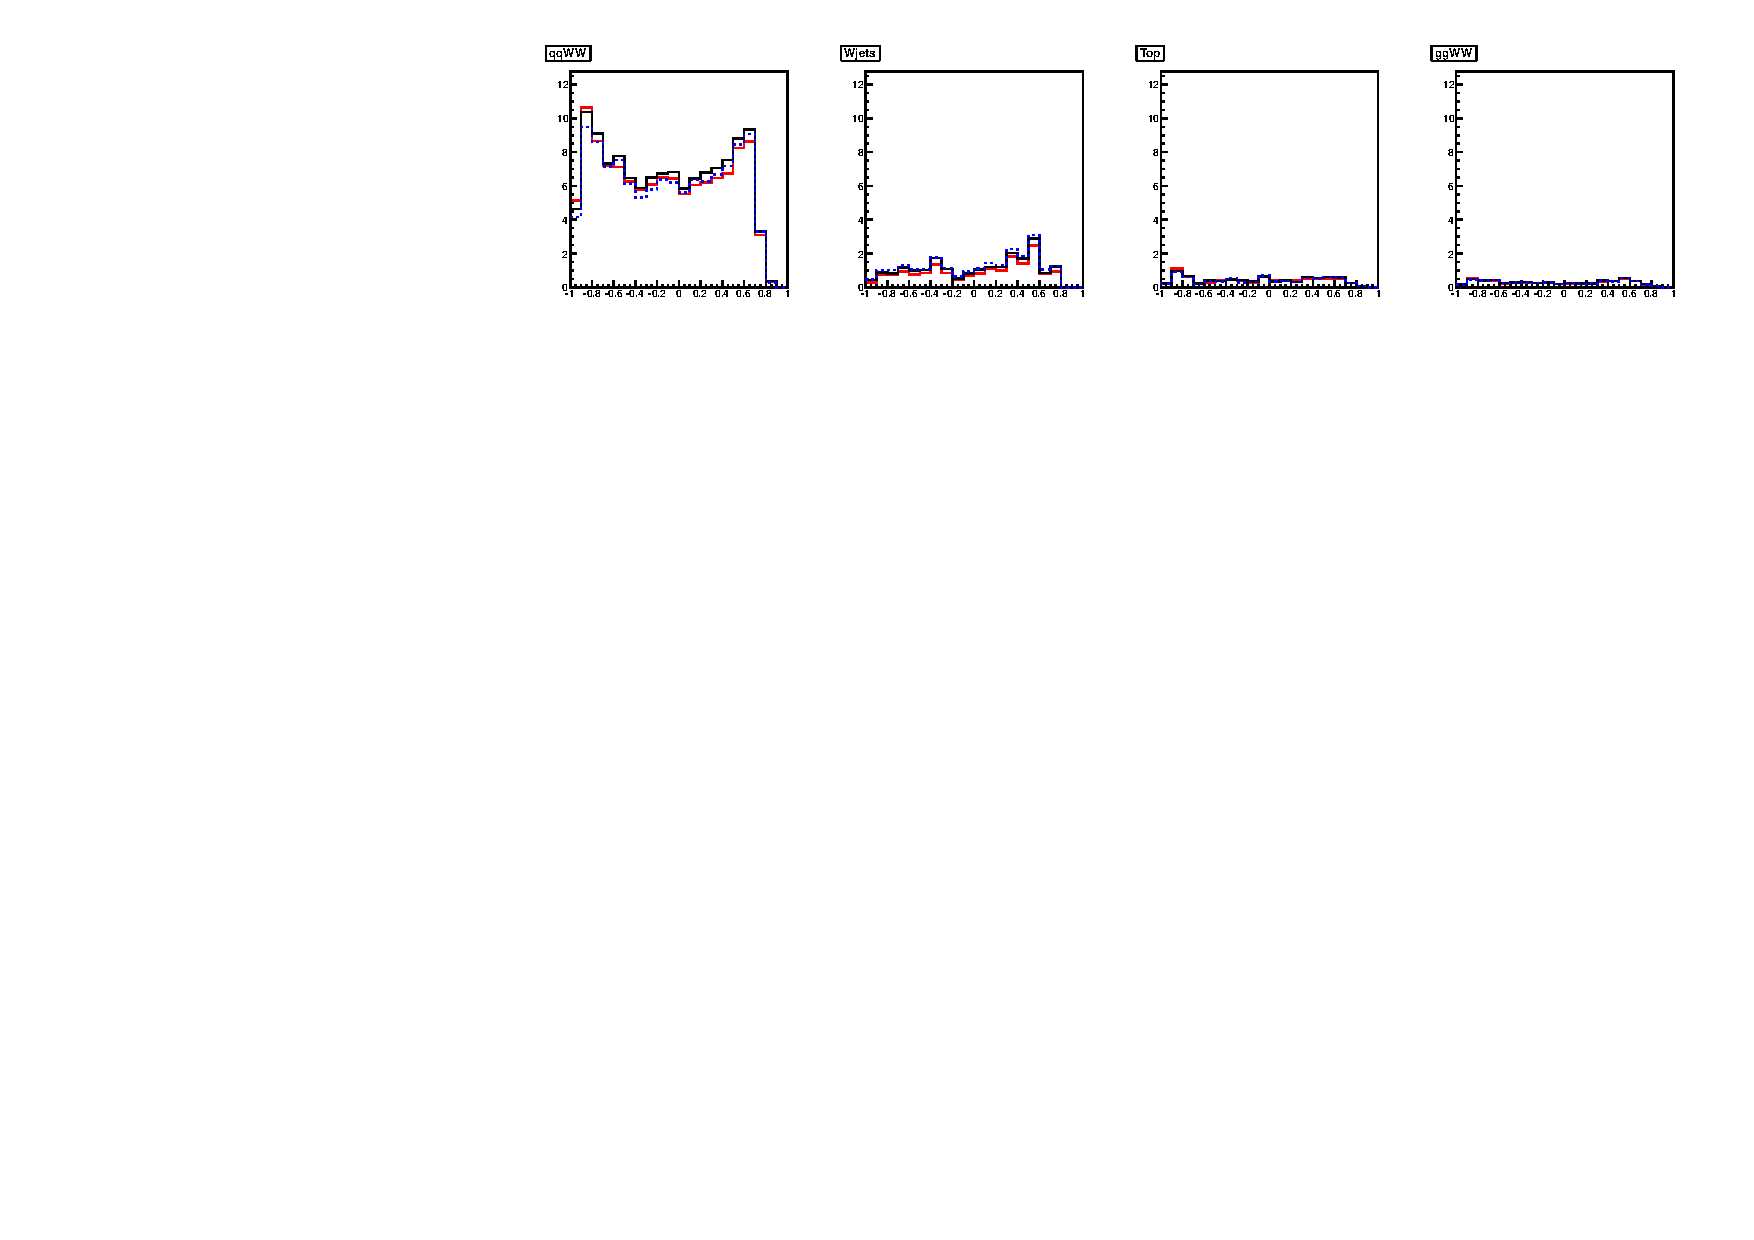
\includegraphics[width=1.0\textwidth]{figures/fits/bdt2_115_n0of.pdf}}\\
\subfigure[$ee$/$\mu\mu$ 0-Jet]{
\centering
\label{subfig:bdt2_115_n0sf}
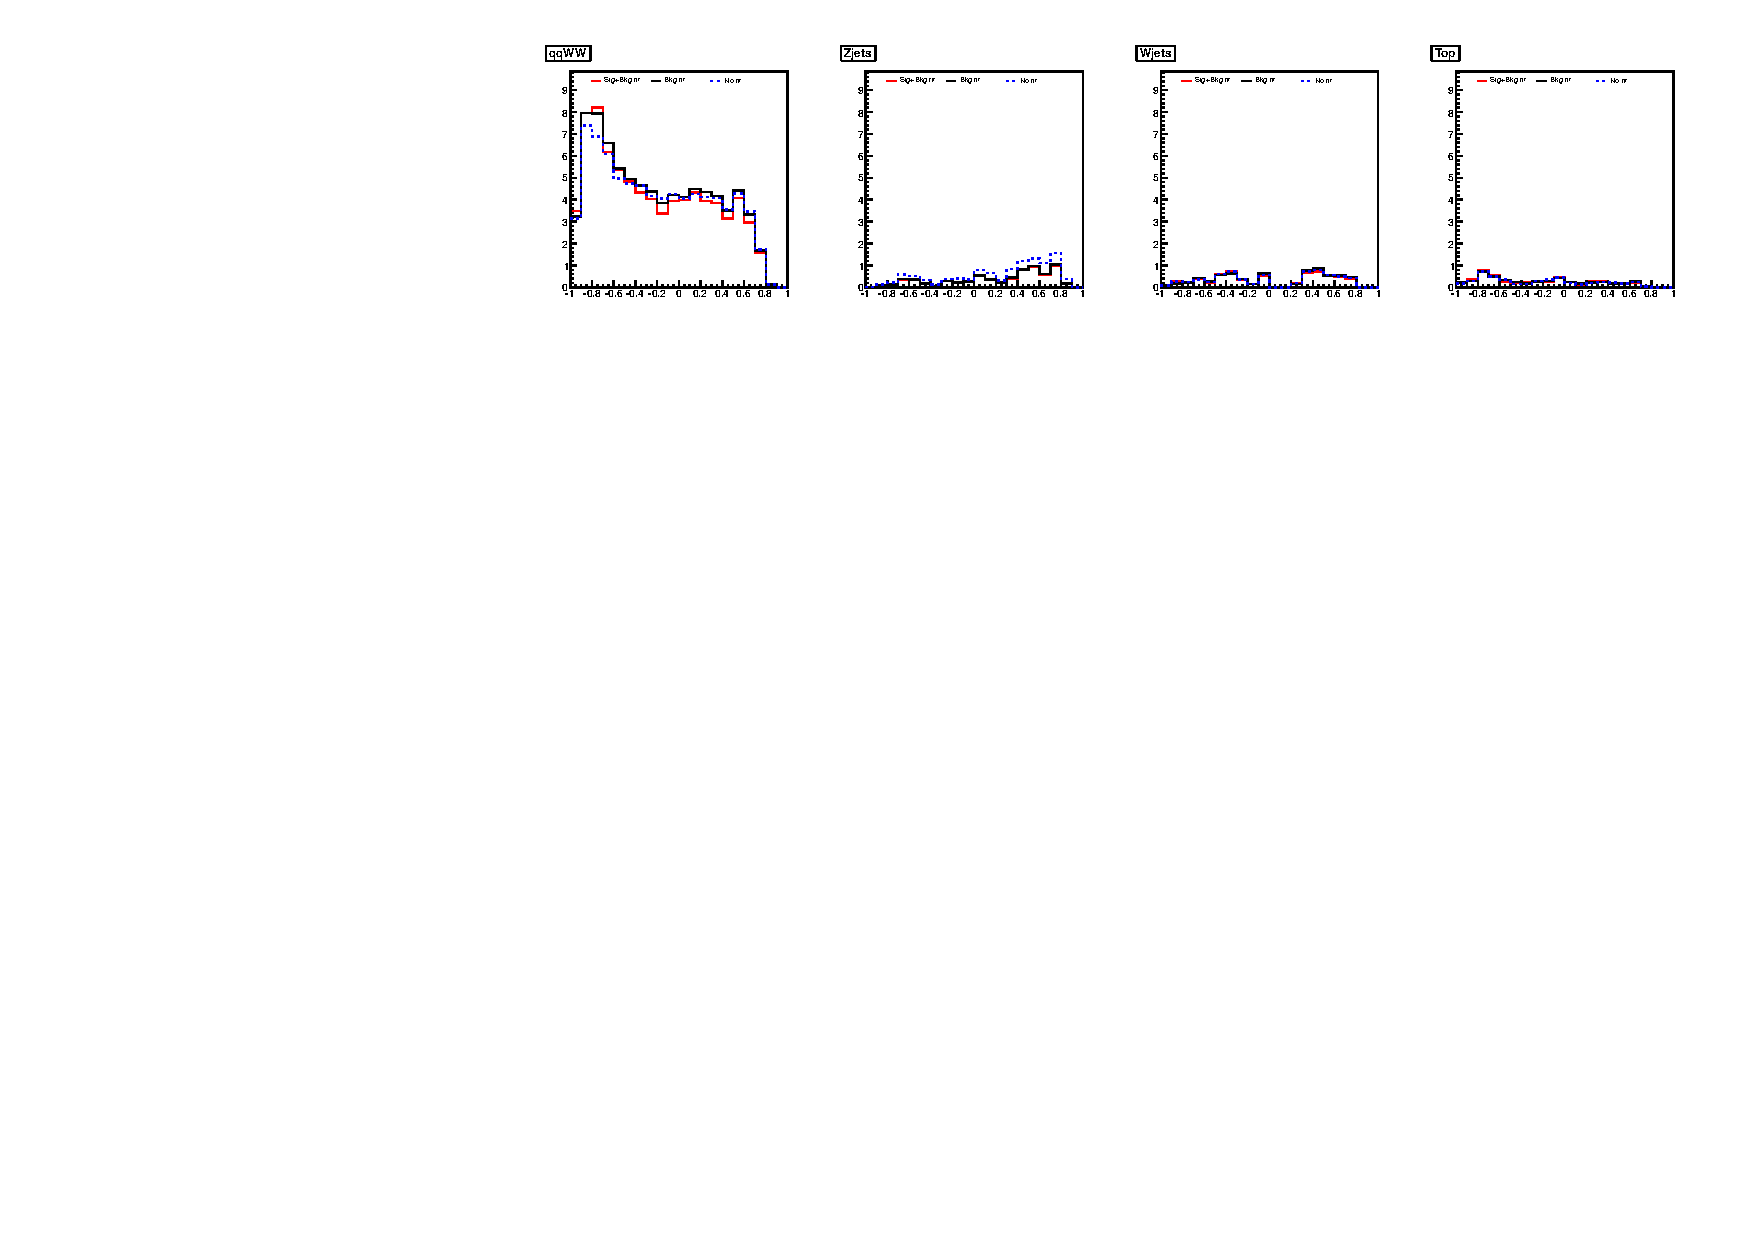
\includegraphics[width=1.0\textwidth]{figures/fits/bdt2_115_n0sf.pdf}}
\subfigure[$e\mu$ 1-Jet]{
\centering
\label{subfig:bdt2_115_n1of}
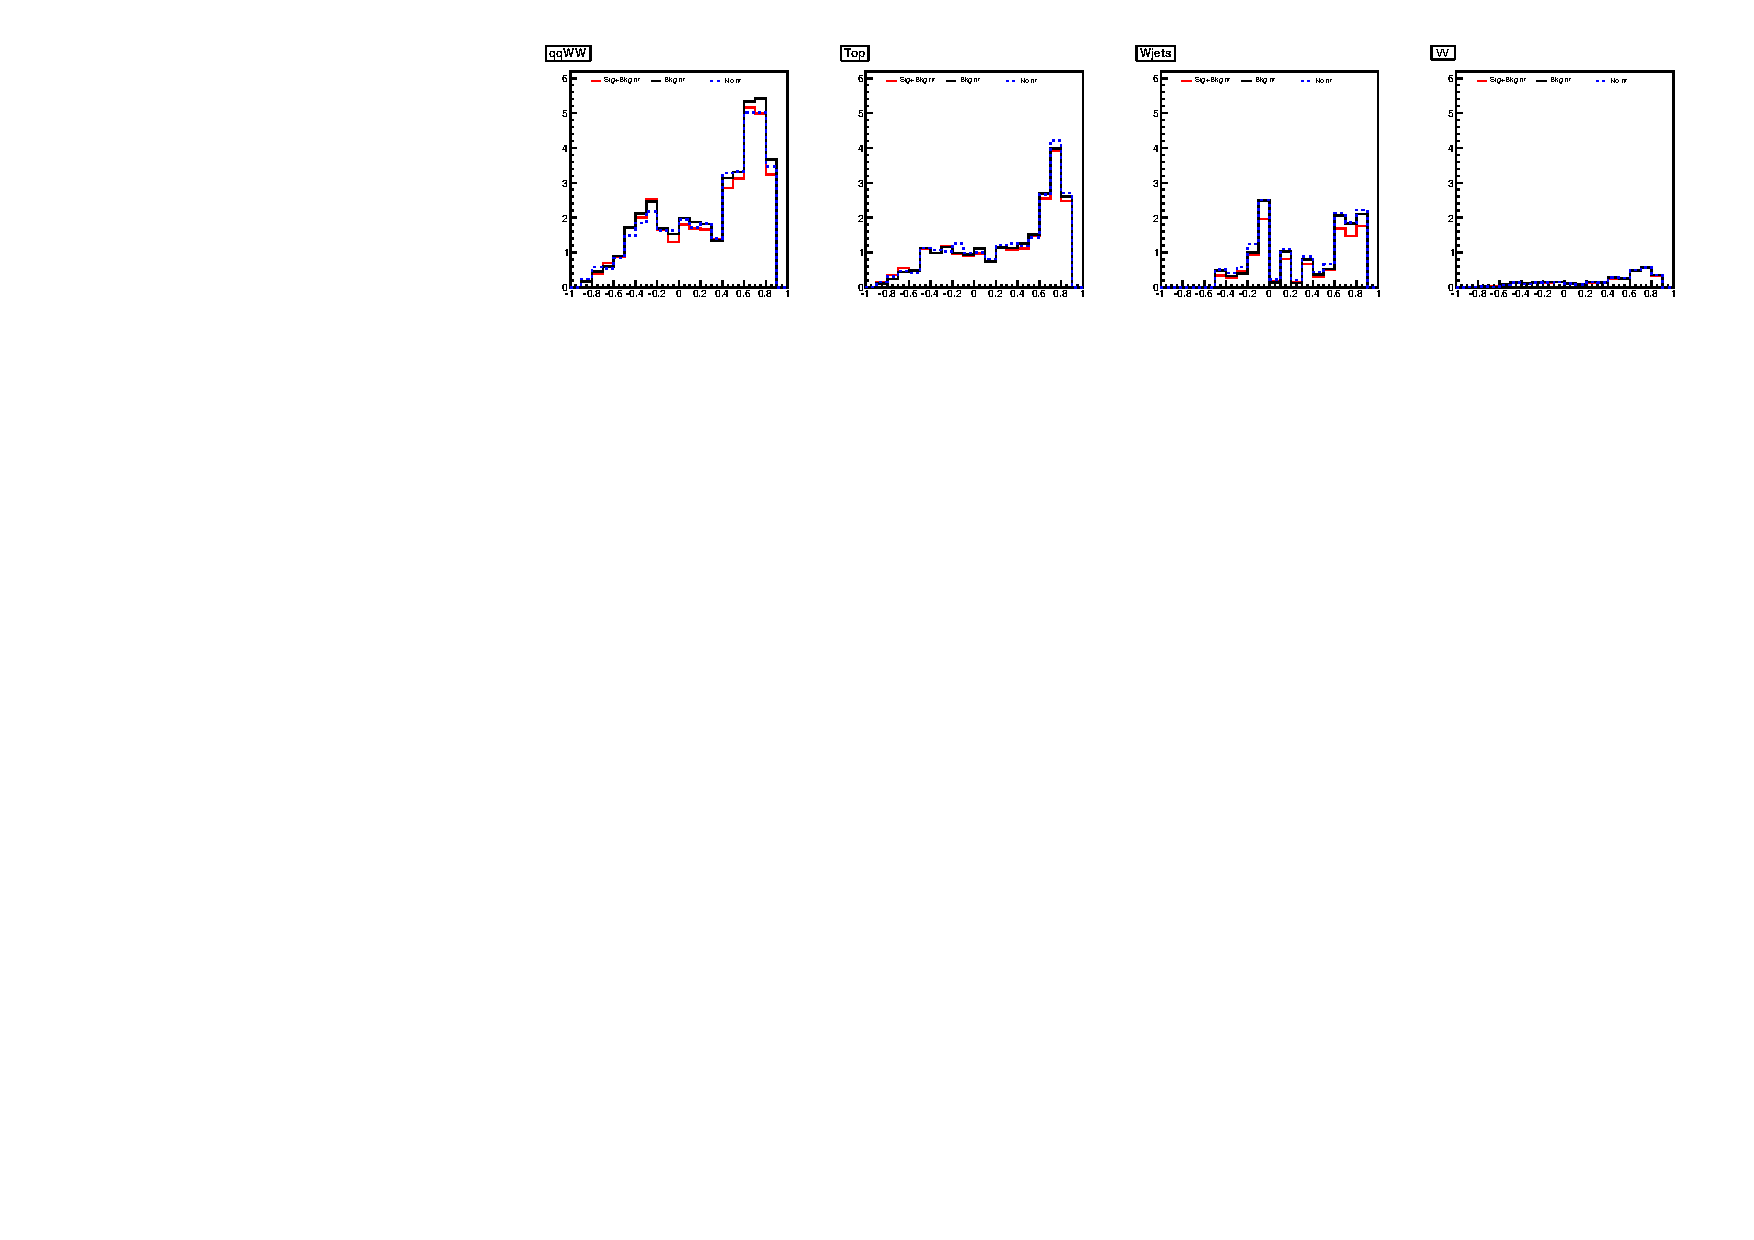
\includegraphics[width=1.0\textwidth]{figures/fits/bdt2_115_n1of.pdf}}\\
\subfigure[$ee$/$\mu\mu$ 1-Jet]{
\centering
\label{subfig:bdt2_115_n1sf}
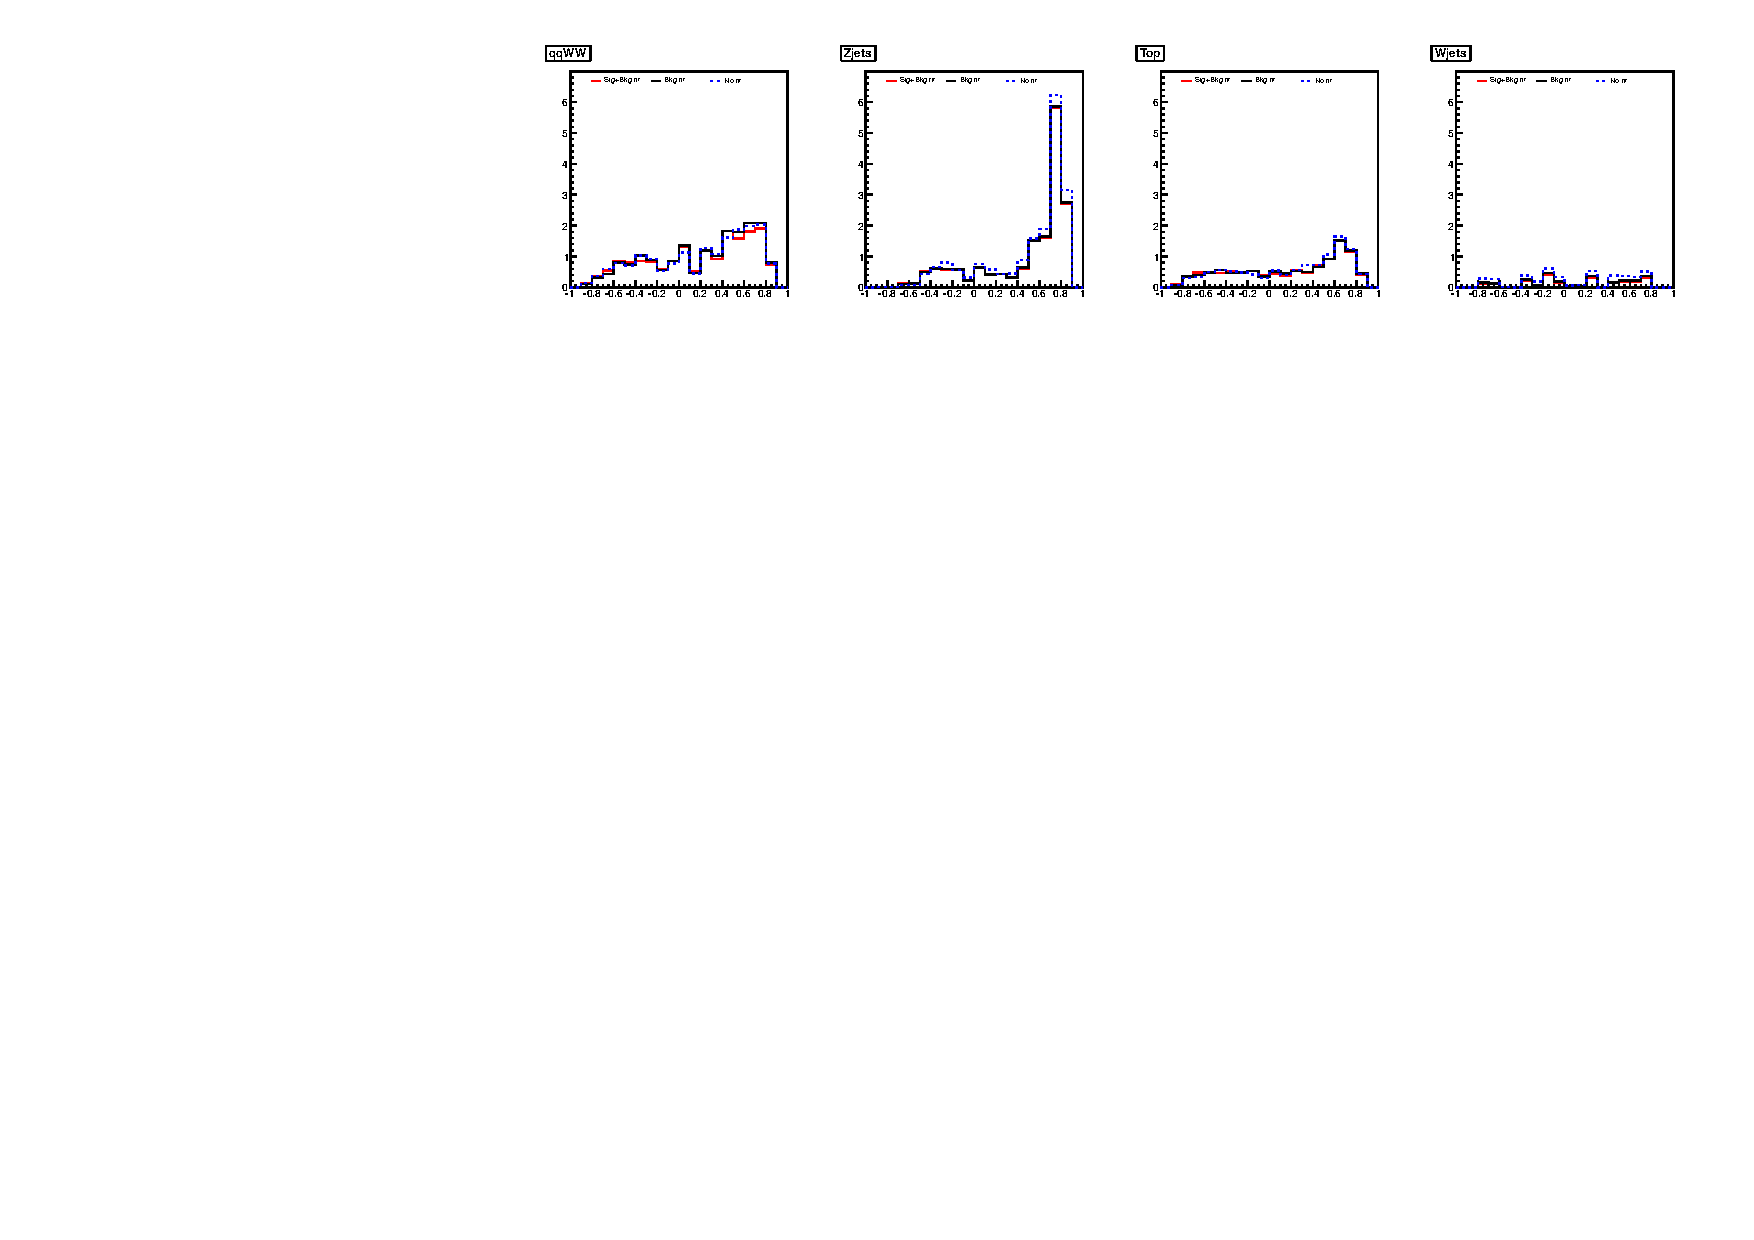
\includegraphics[width=1.0\textwidth]{figures/fits/bdt2_115_n1sf.pdf}}
\caption{
MVA output distributions for dominant background contributions for
Higgs 115~\GeV\ without fitting (nominal), background fit (signal is
set to zero) and signal+background fit (signal is floating in the
fit).}
\label{fig:bdt2_115}
\end{figure}

\begin{figure}[!hbtp]
\centering
\subfigure[$e\mu$ 0-Jet]{
\centering
\label{subfig:bdt2_120_n0of}
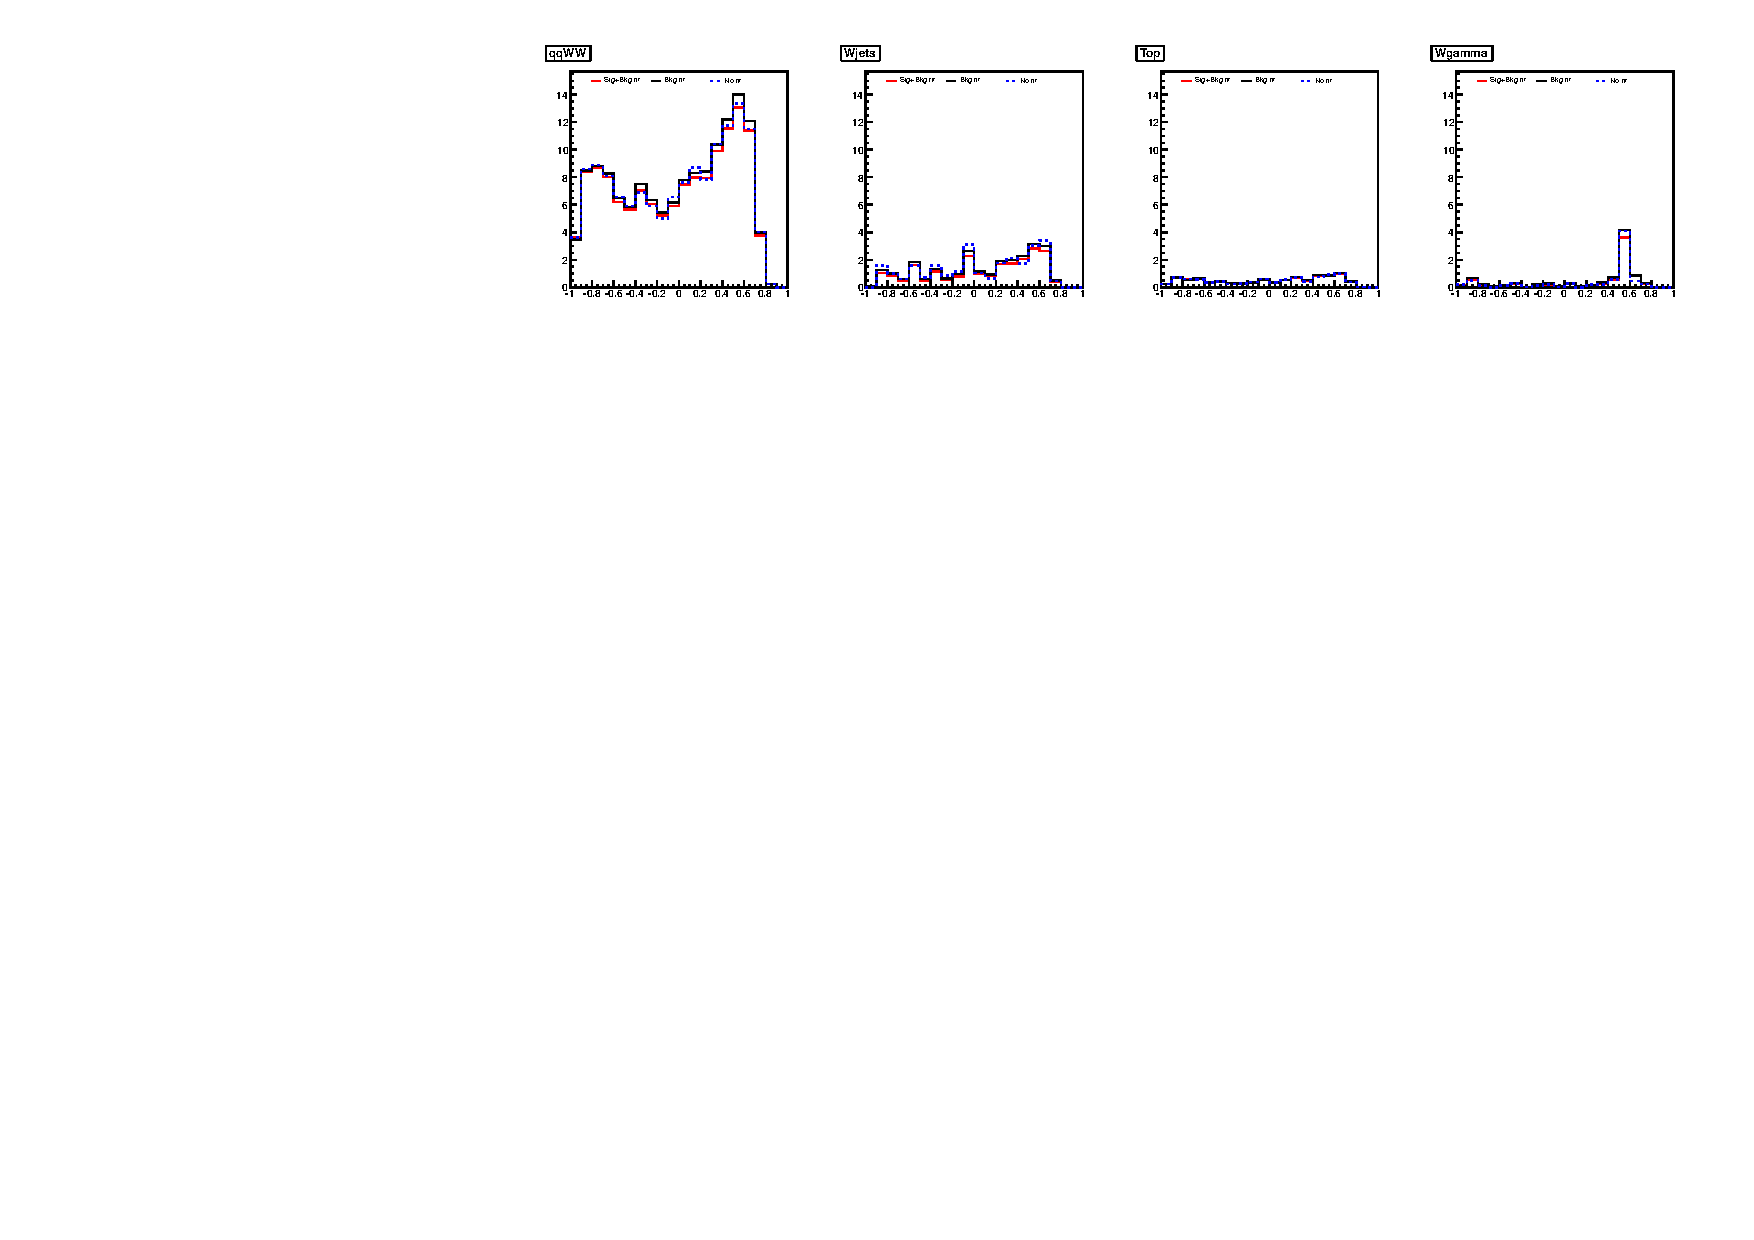
\includegraphics[width=1.0\textwidth]{figures/fits/bdt2_120_n0of.pdf}}\\
\subfigure[$ee$/$\mu\mu$ 0-Jet]{
\centering
\label{subfig:bdt2_120_n0sf}
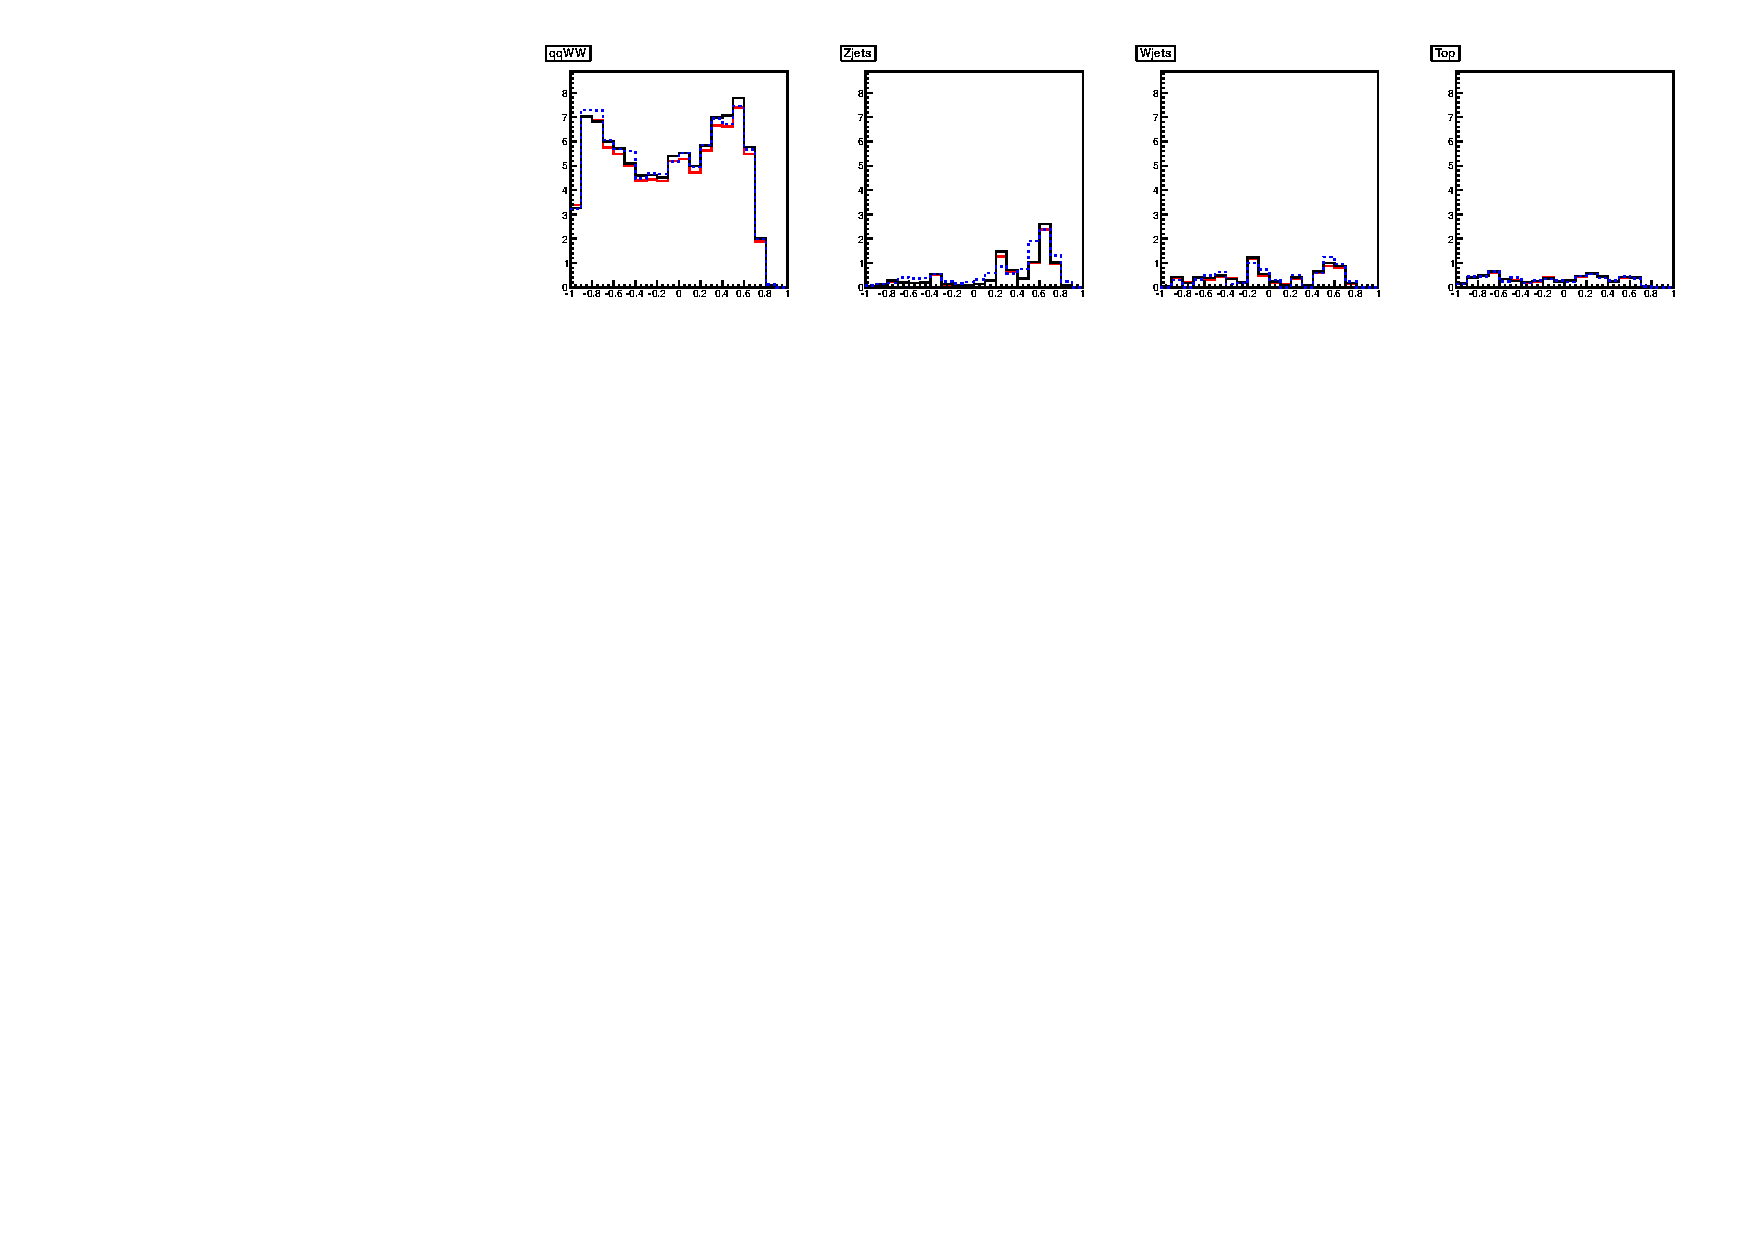
\includegraphics[width=1.0\textwidth]{figures/fits/bdt2_120_n0sf.pdf}}
\subfigure[$e\mu$ 1-Jet]{
\centering
\label{subfig:bdt2_120_n1of}
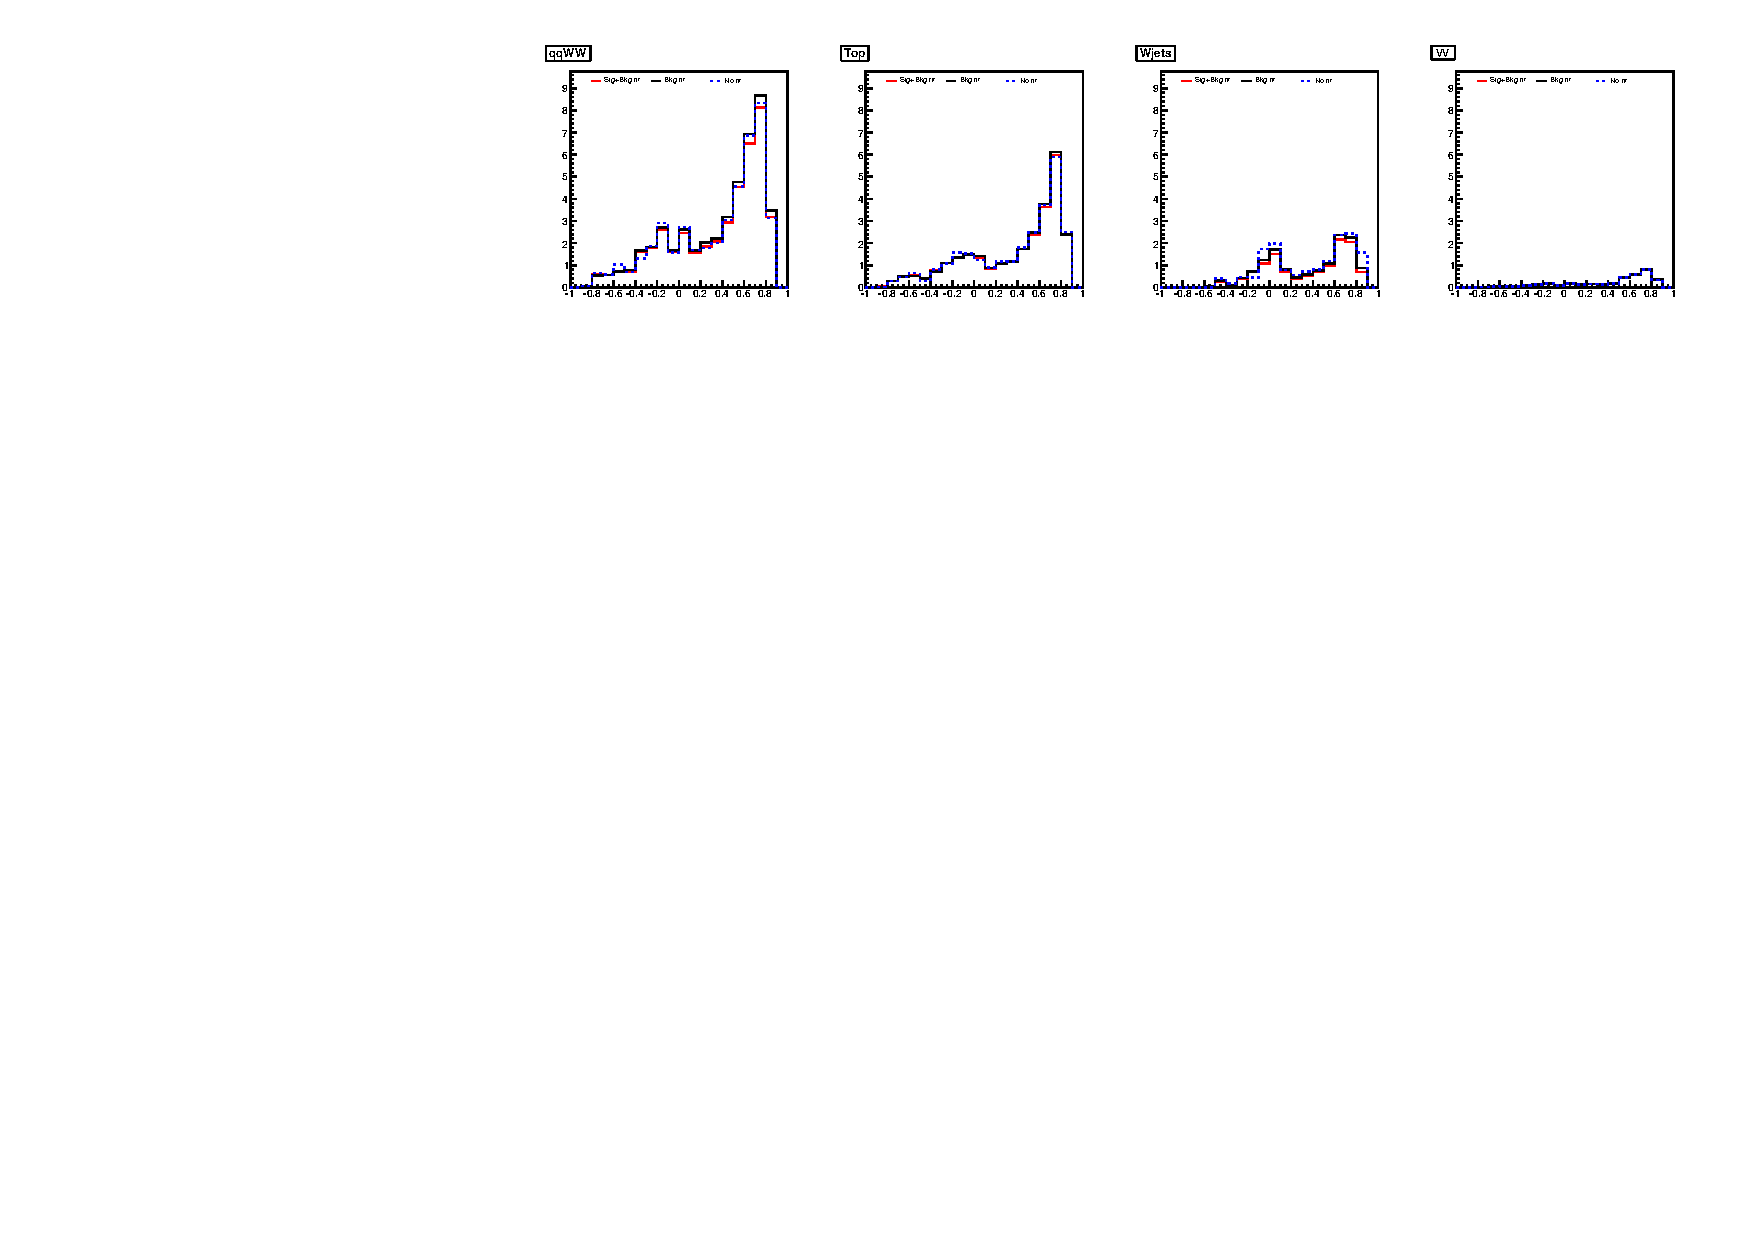
\includegraphics[width=1.0\textwidth]{figures/fits/bdt2_120_n1of.pdf}}\\
\subfigure[$ee$/$\mu\mu$ 1-Jet]{
\centering
\label{subfig:bdt2_120_n1sf}
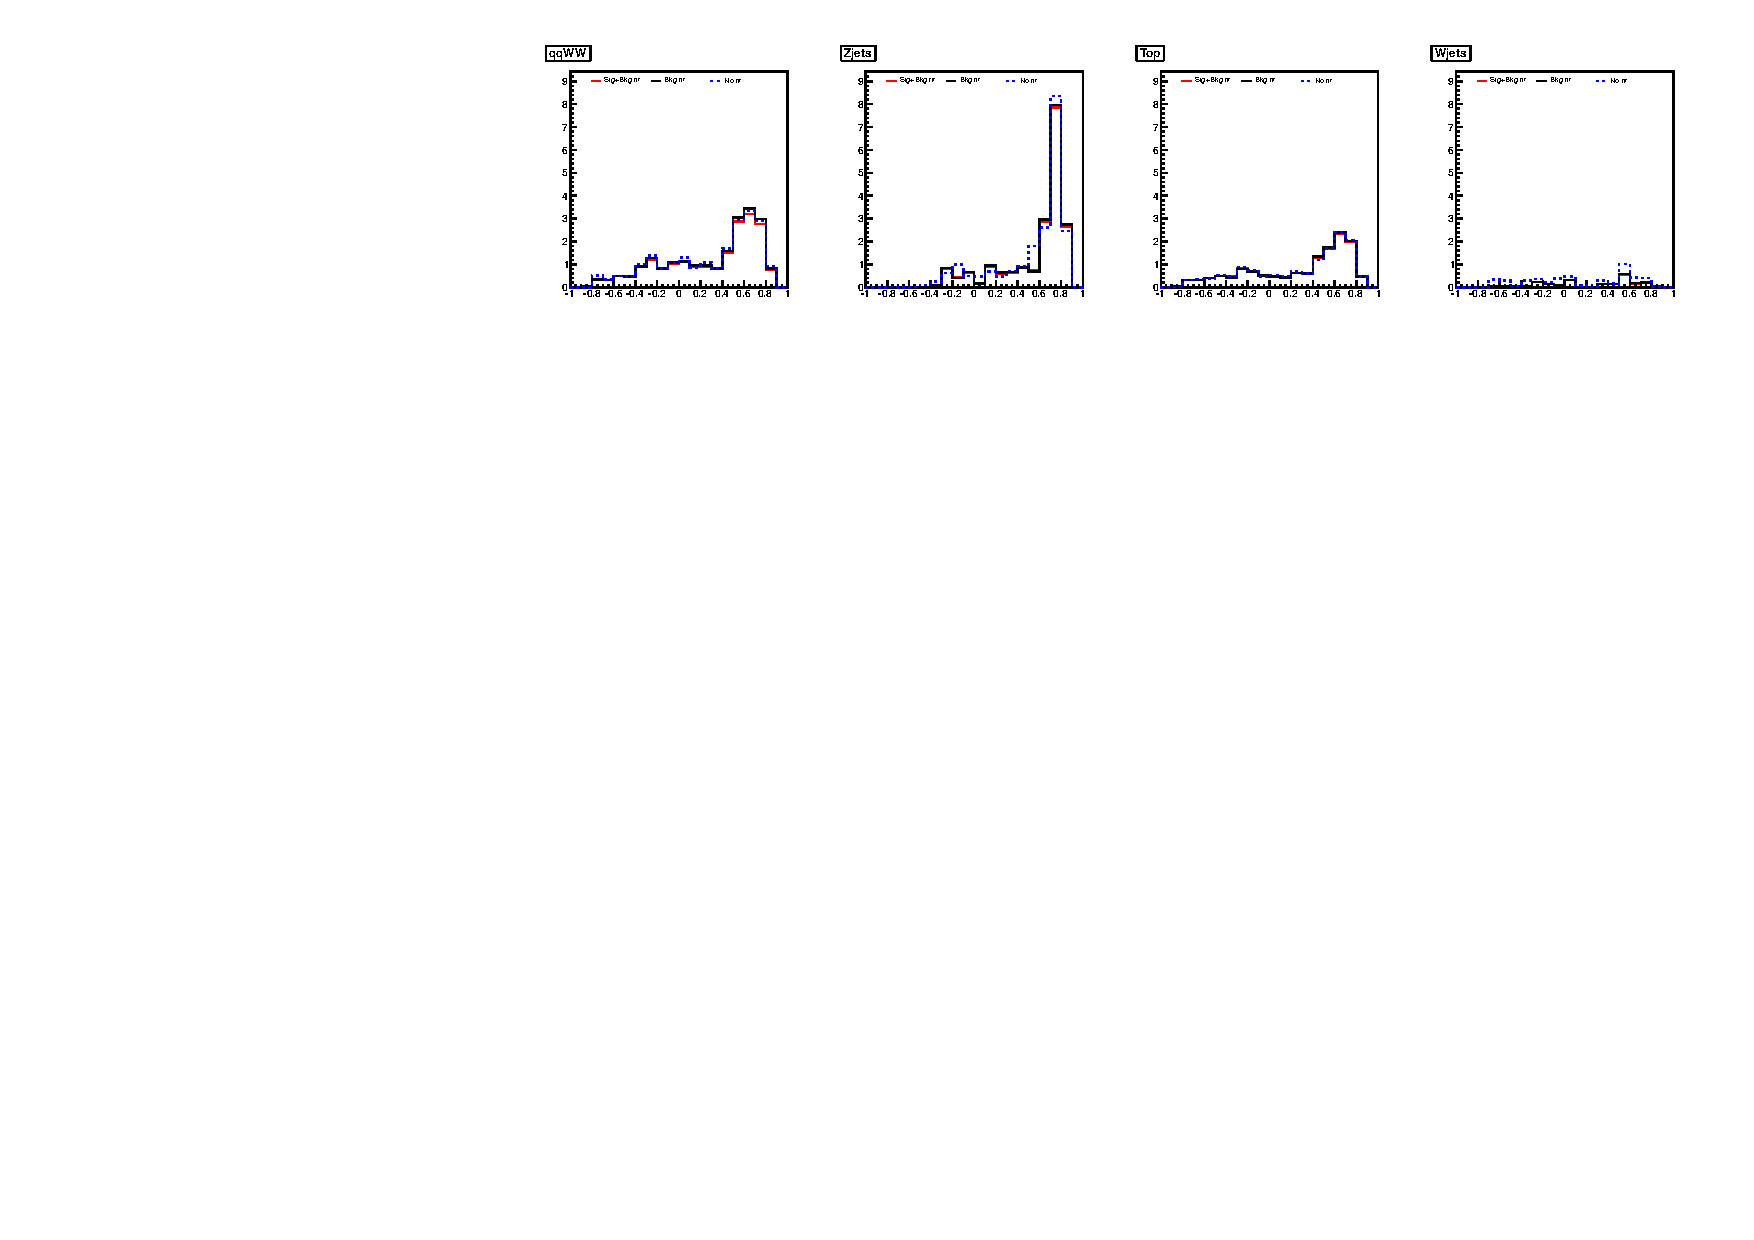
\includegraphics[width=1.0\textwidth]{figures/fits/bdt2_120_n1sf.pdf}}
\caption{
MVA output distributions for dominant background contributions for
Higgs 120~\GeV\ without fitting (nominal), background fit (signal is
set to zero) and signal+background fit (signal is floating in the
fit).}
\label{fig:bdt2_120}
\end{figure}

\begin{figure}[!hbtp]
\centering
\subfigure[$e\mu$ 0-Jet]{
\centering
\label{subfig:bdt2_130_n0of}
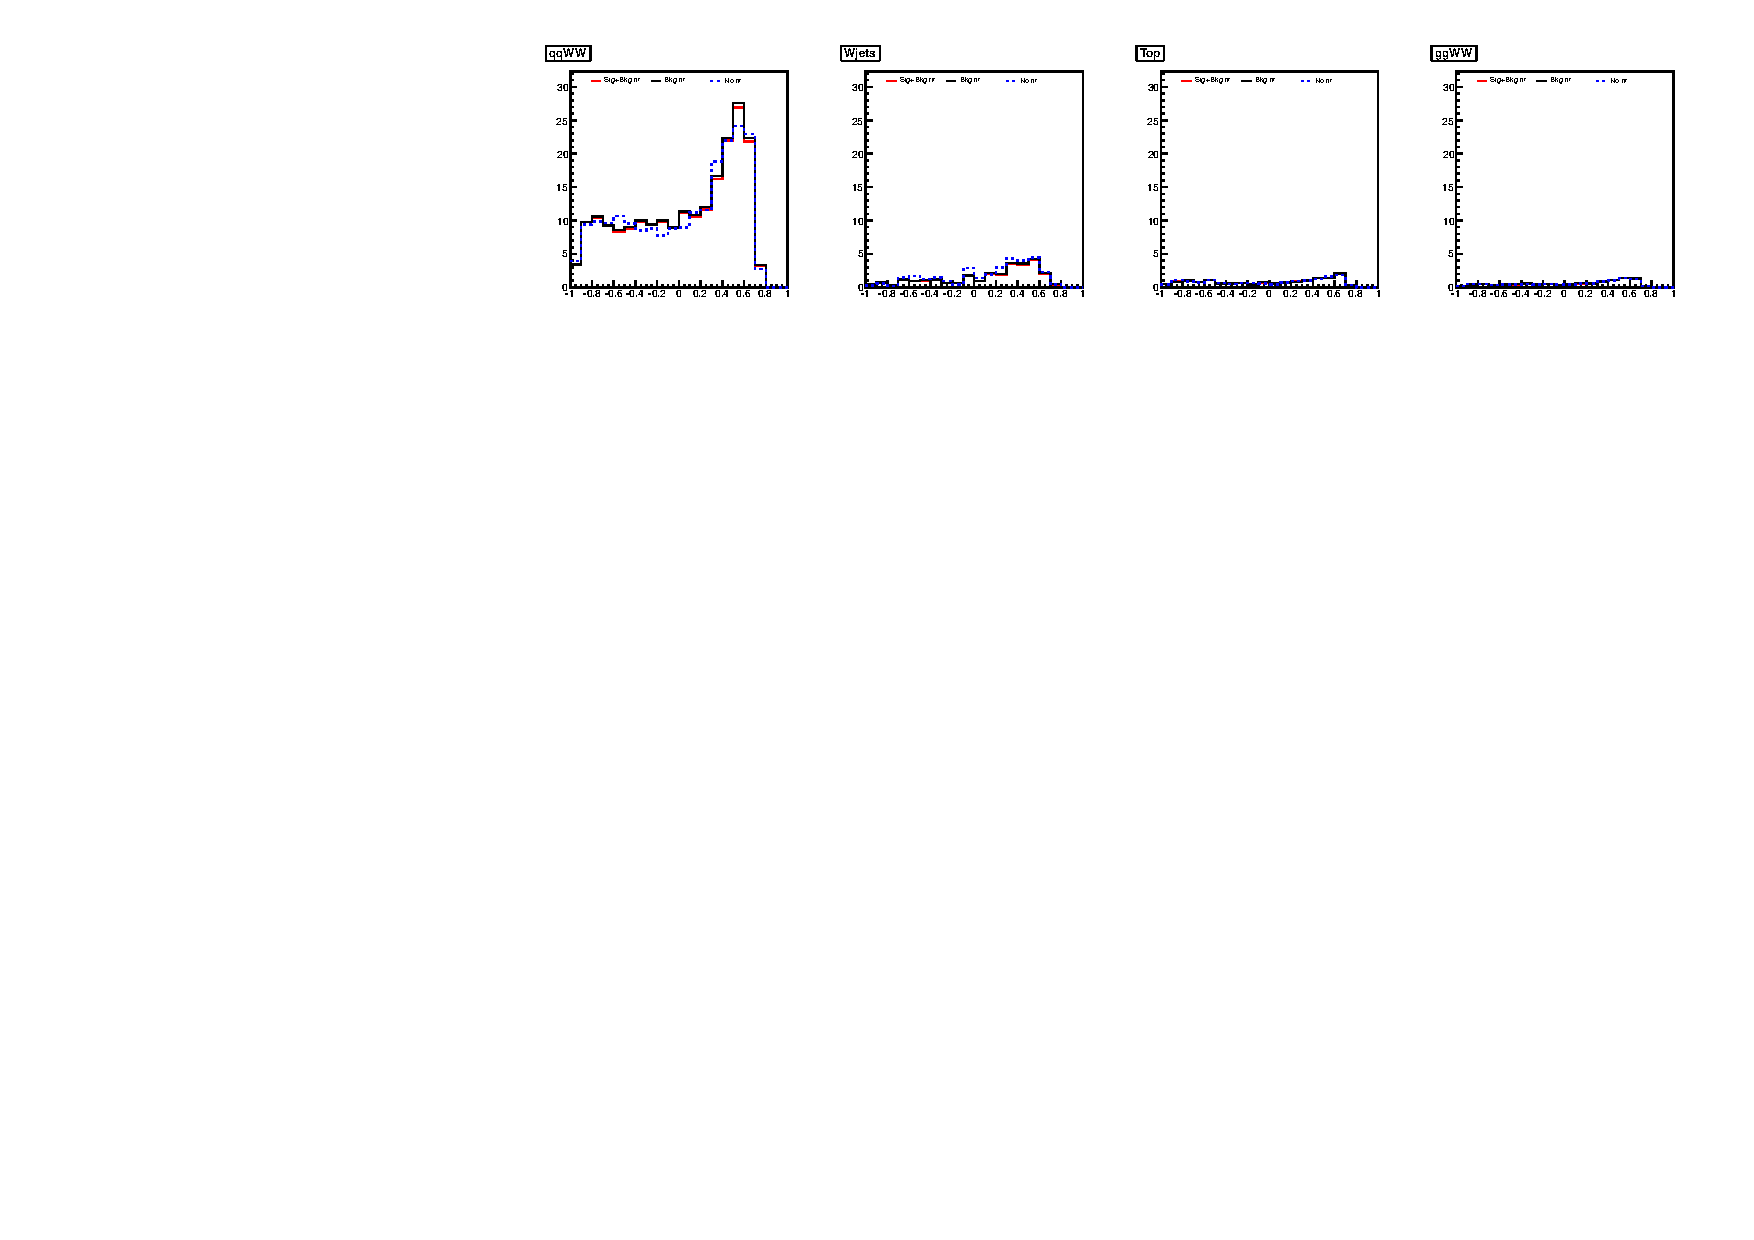
\includegraphics[width=1.0\textwidth]{figures/fits/bdt2_130_n0of.pdf}}\\
\subfigure[$ee$/$\mu\mu$ 0-Jet]{
\centering
\label{subfig:bdt2_130_n0sf}
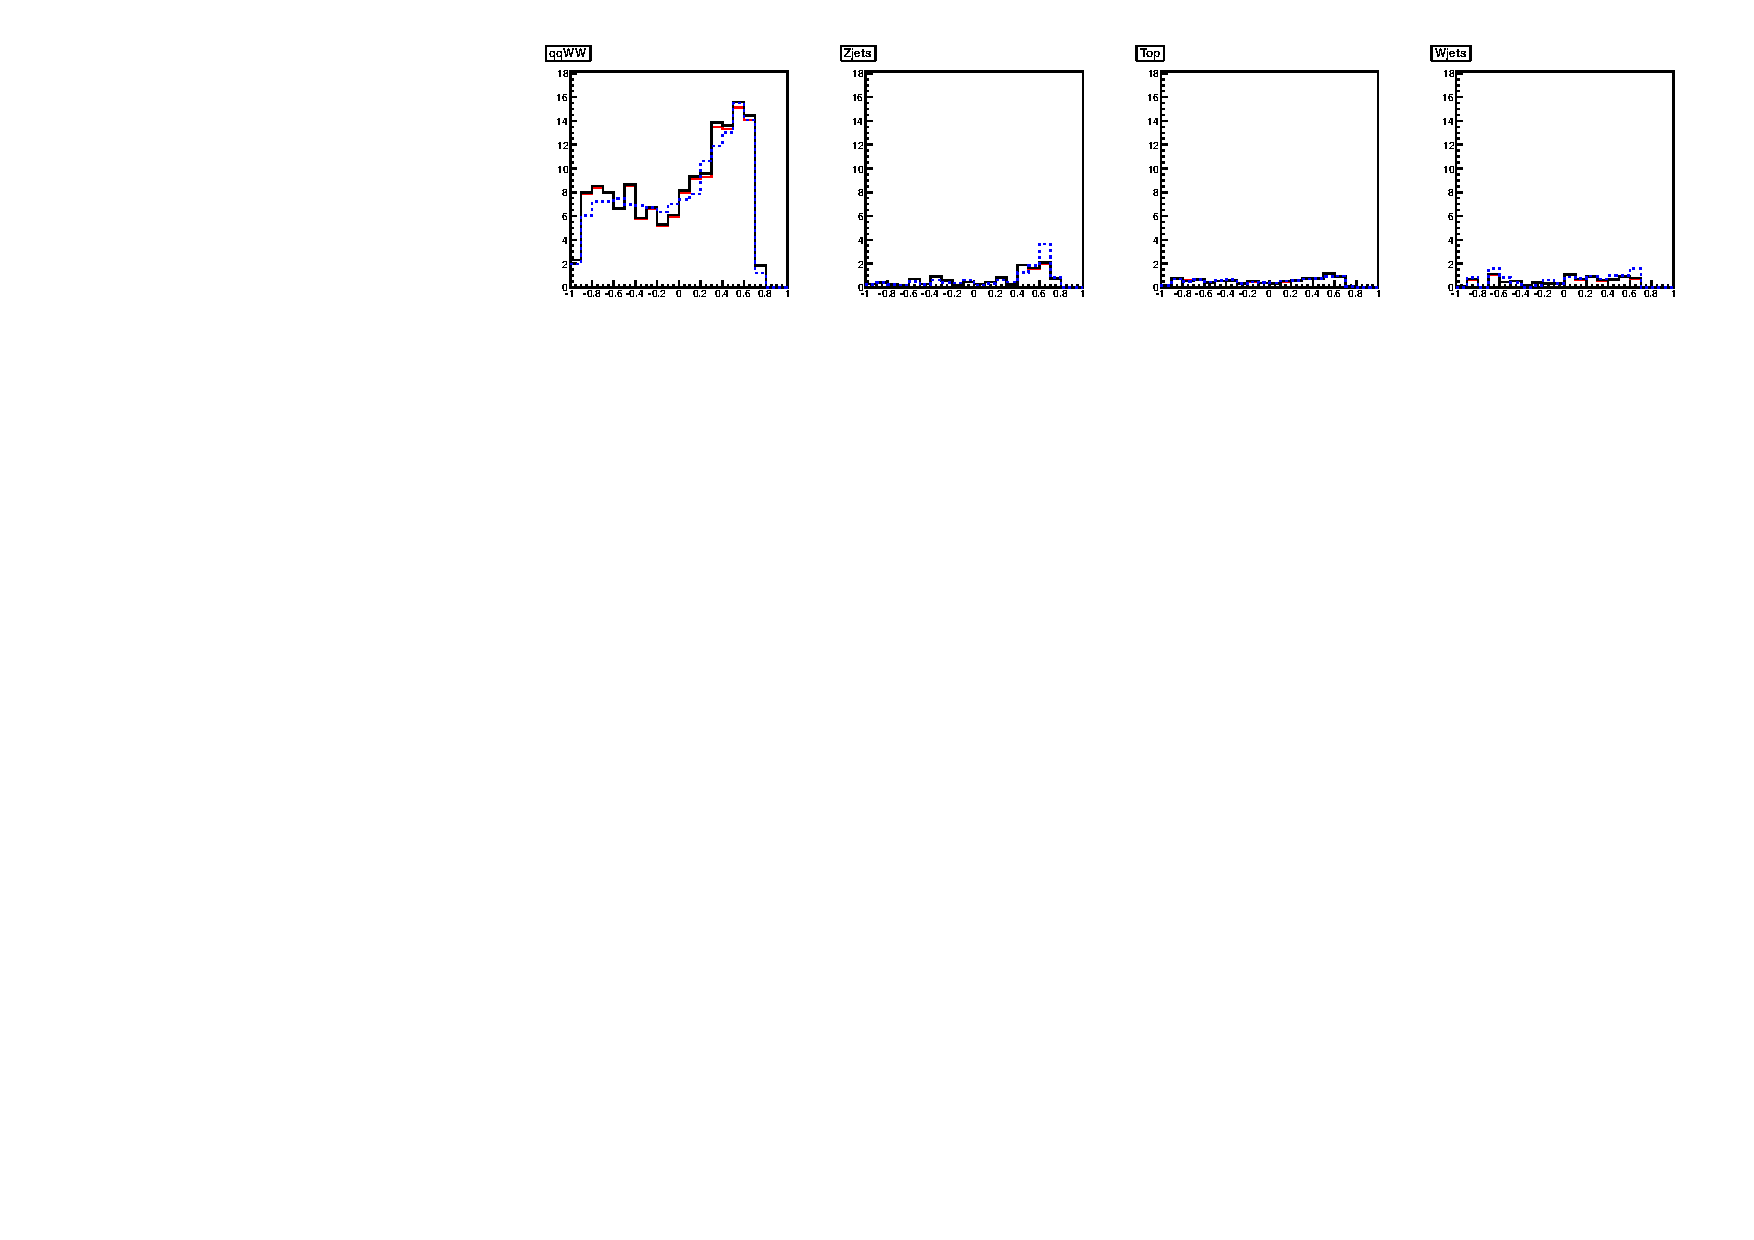
\includegraphics[width=1.0\textwidth]{figures/fits/bdt2_130_n0sf.pdf}}
\subfigure[$e\mu$ 1-Jet]{
\centering
\label{subfig:bdt2_130_n1of}
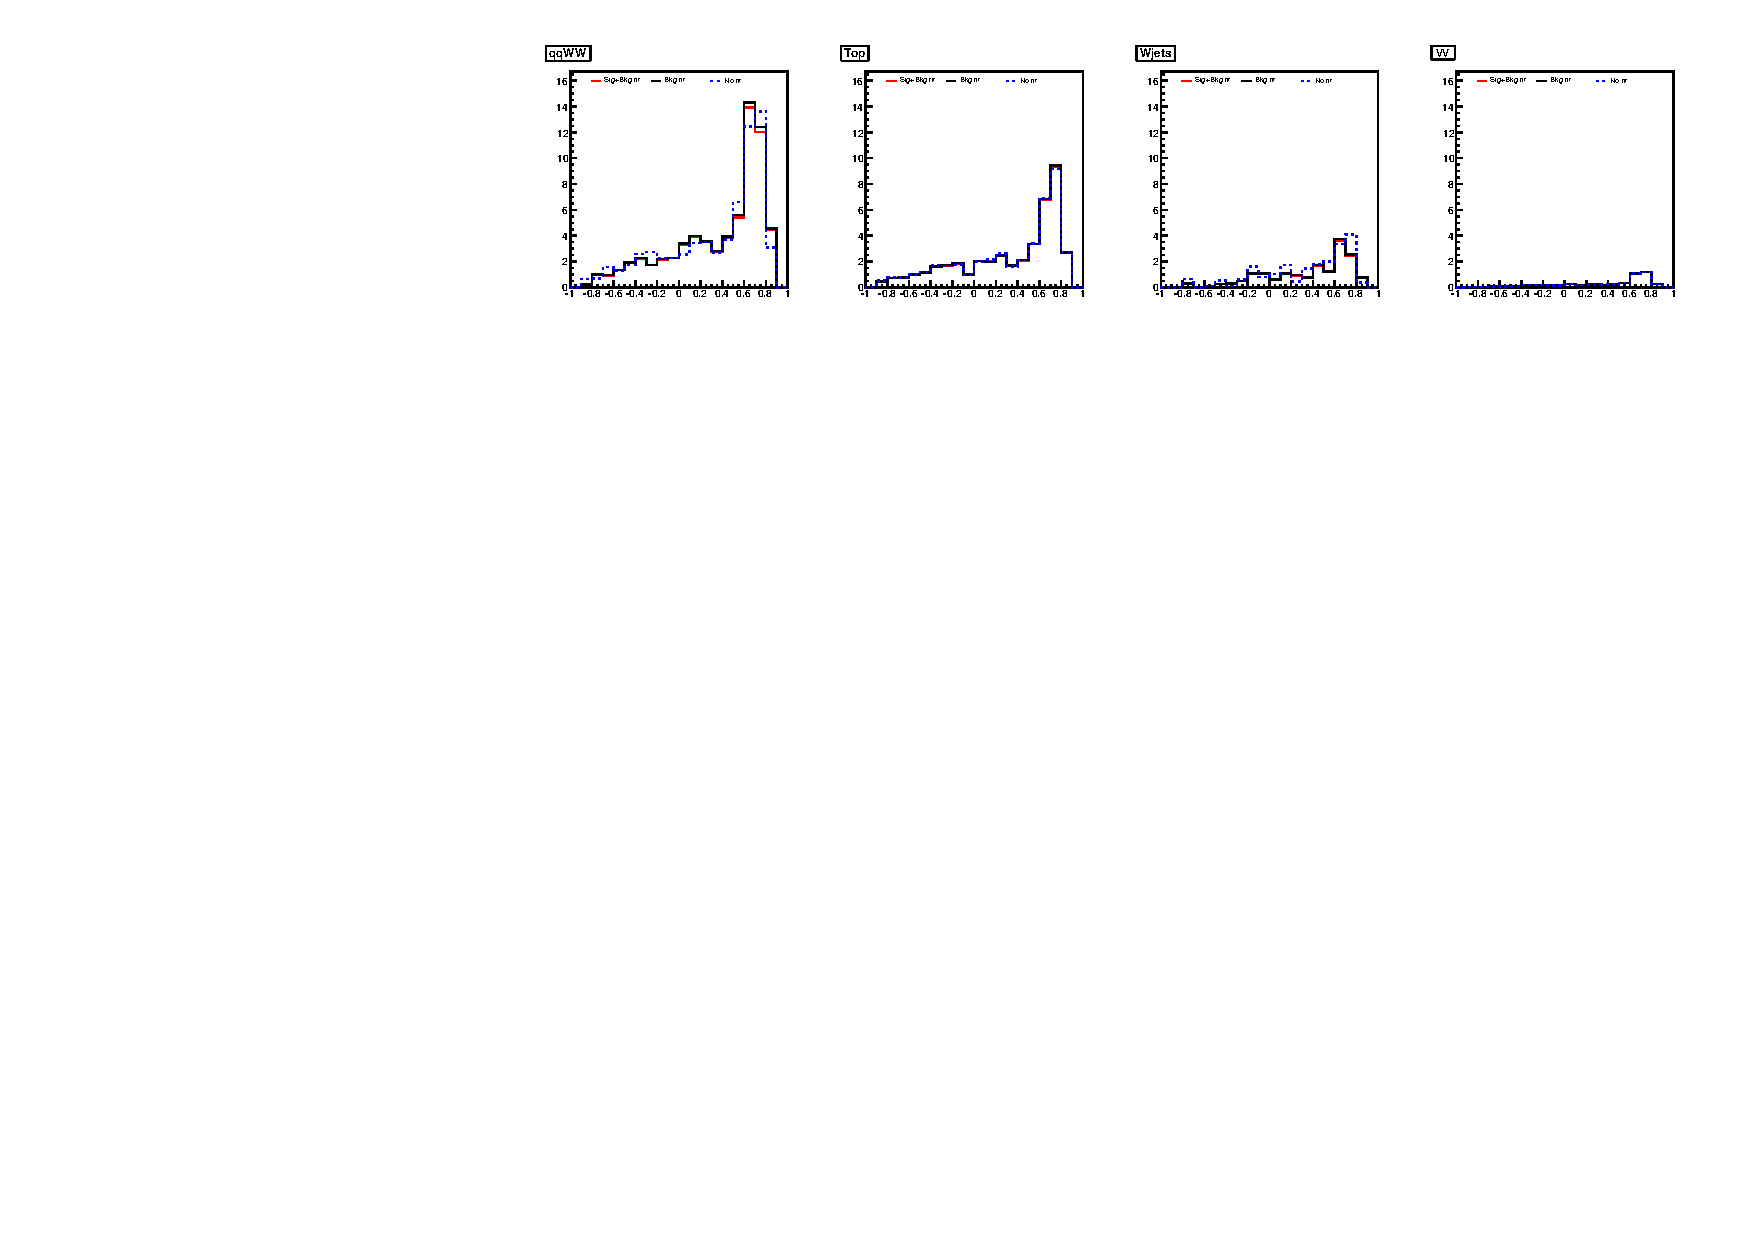
\includegraphics[width=1.0\textwidth]{figures/fits/bdt2_130_n1of.pdf}}\\
\subfigure[$ee$/$\mu\mu$ 1-Jet]{
\centering
\label{subfig:bdt2_130_n1sf}
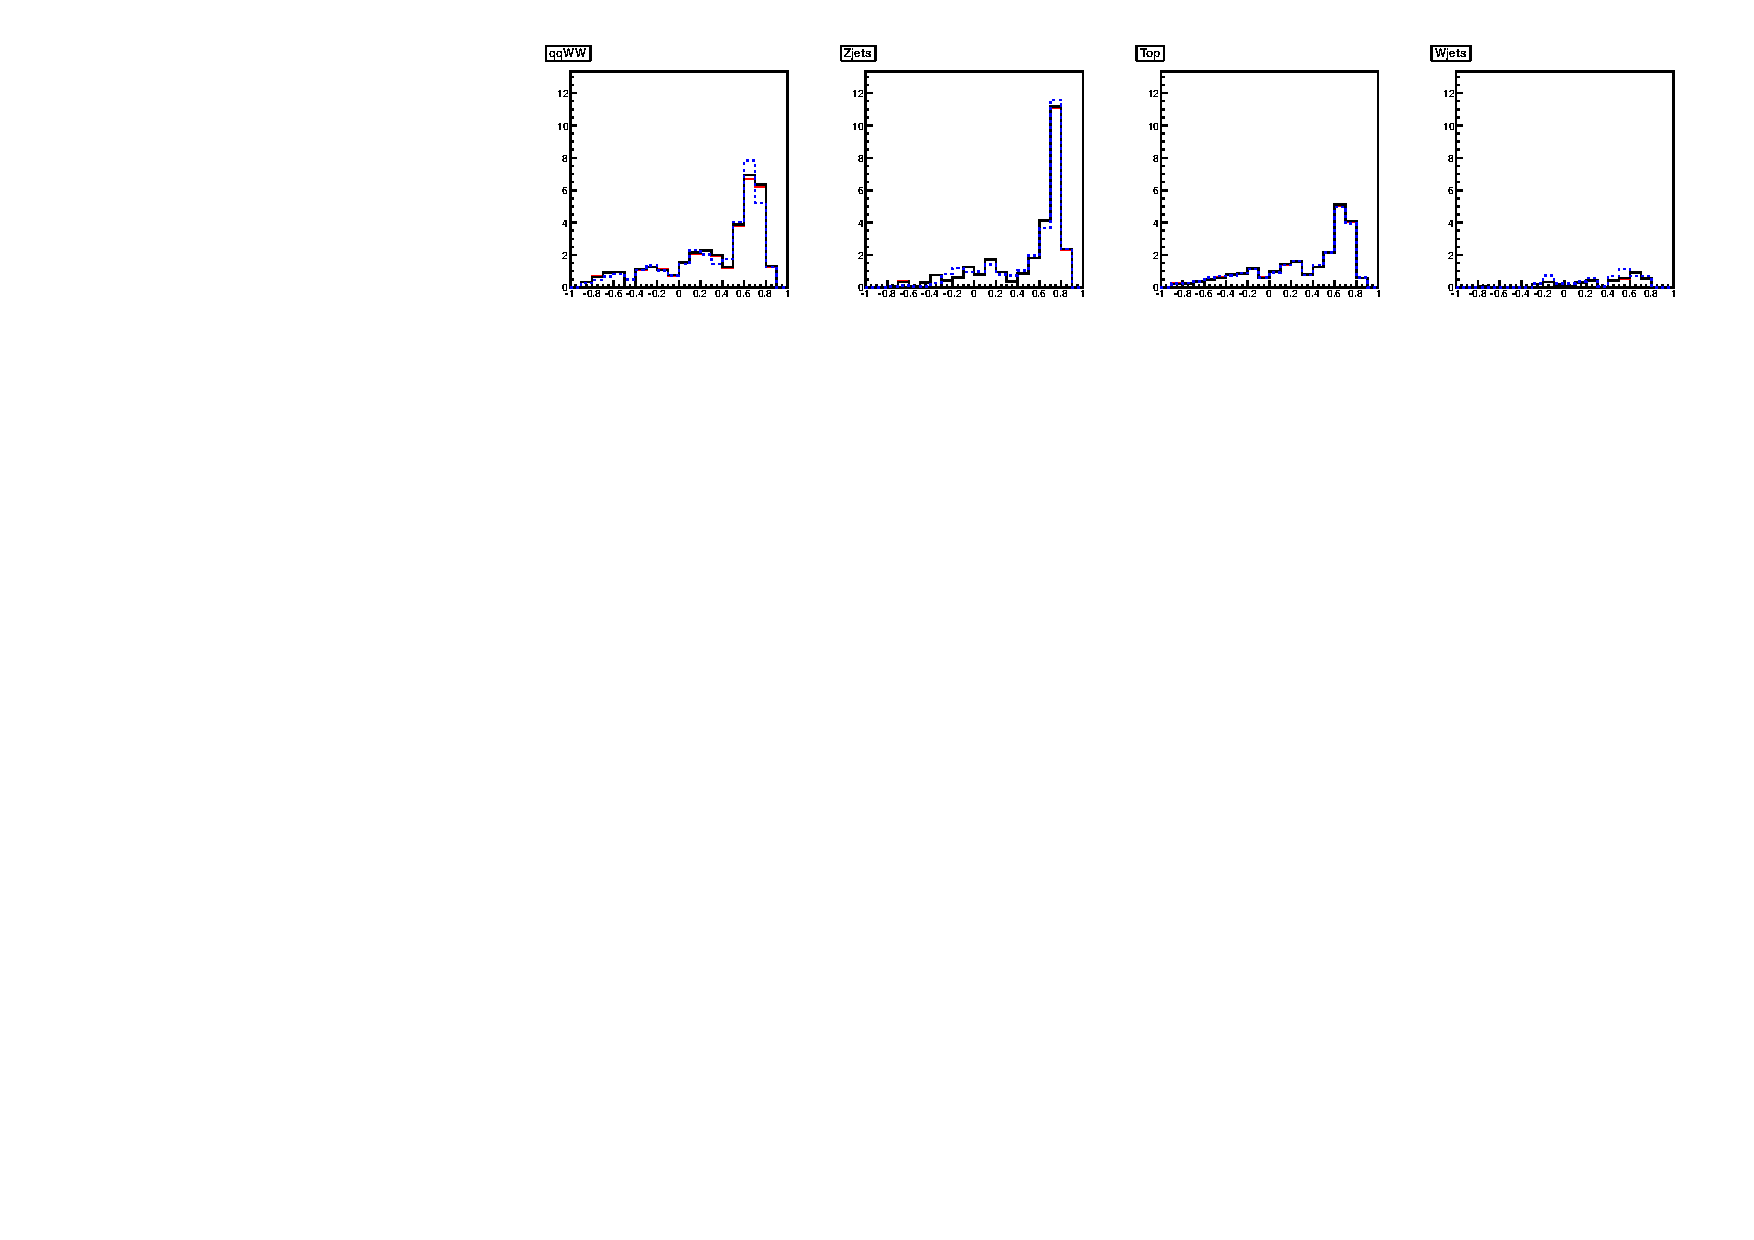
\includegraphics[width=1.0\textwidth]{figures/fits/bdt2_130_n1sf.pdf}}
\caption{
MVA output distributions for dominant background contributions for
Higgs 130~\GeV\ without fitting (nominal), background fit (signal is
set to zero) and signal+background fit (signal is floating in the
fit).}
\label{fig:bdt2_130}
\end{figure}

\begin{figure}[!hbtp]
\centering
\subfigure[$e\mu$ 0-Jet]{
\centering
\label{subfig:bdt2_350_n0of}
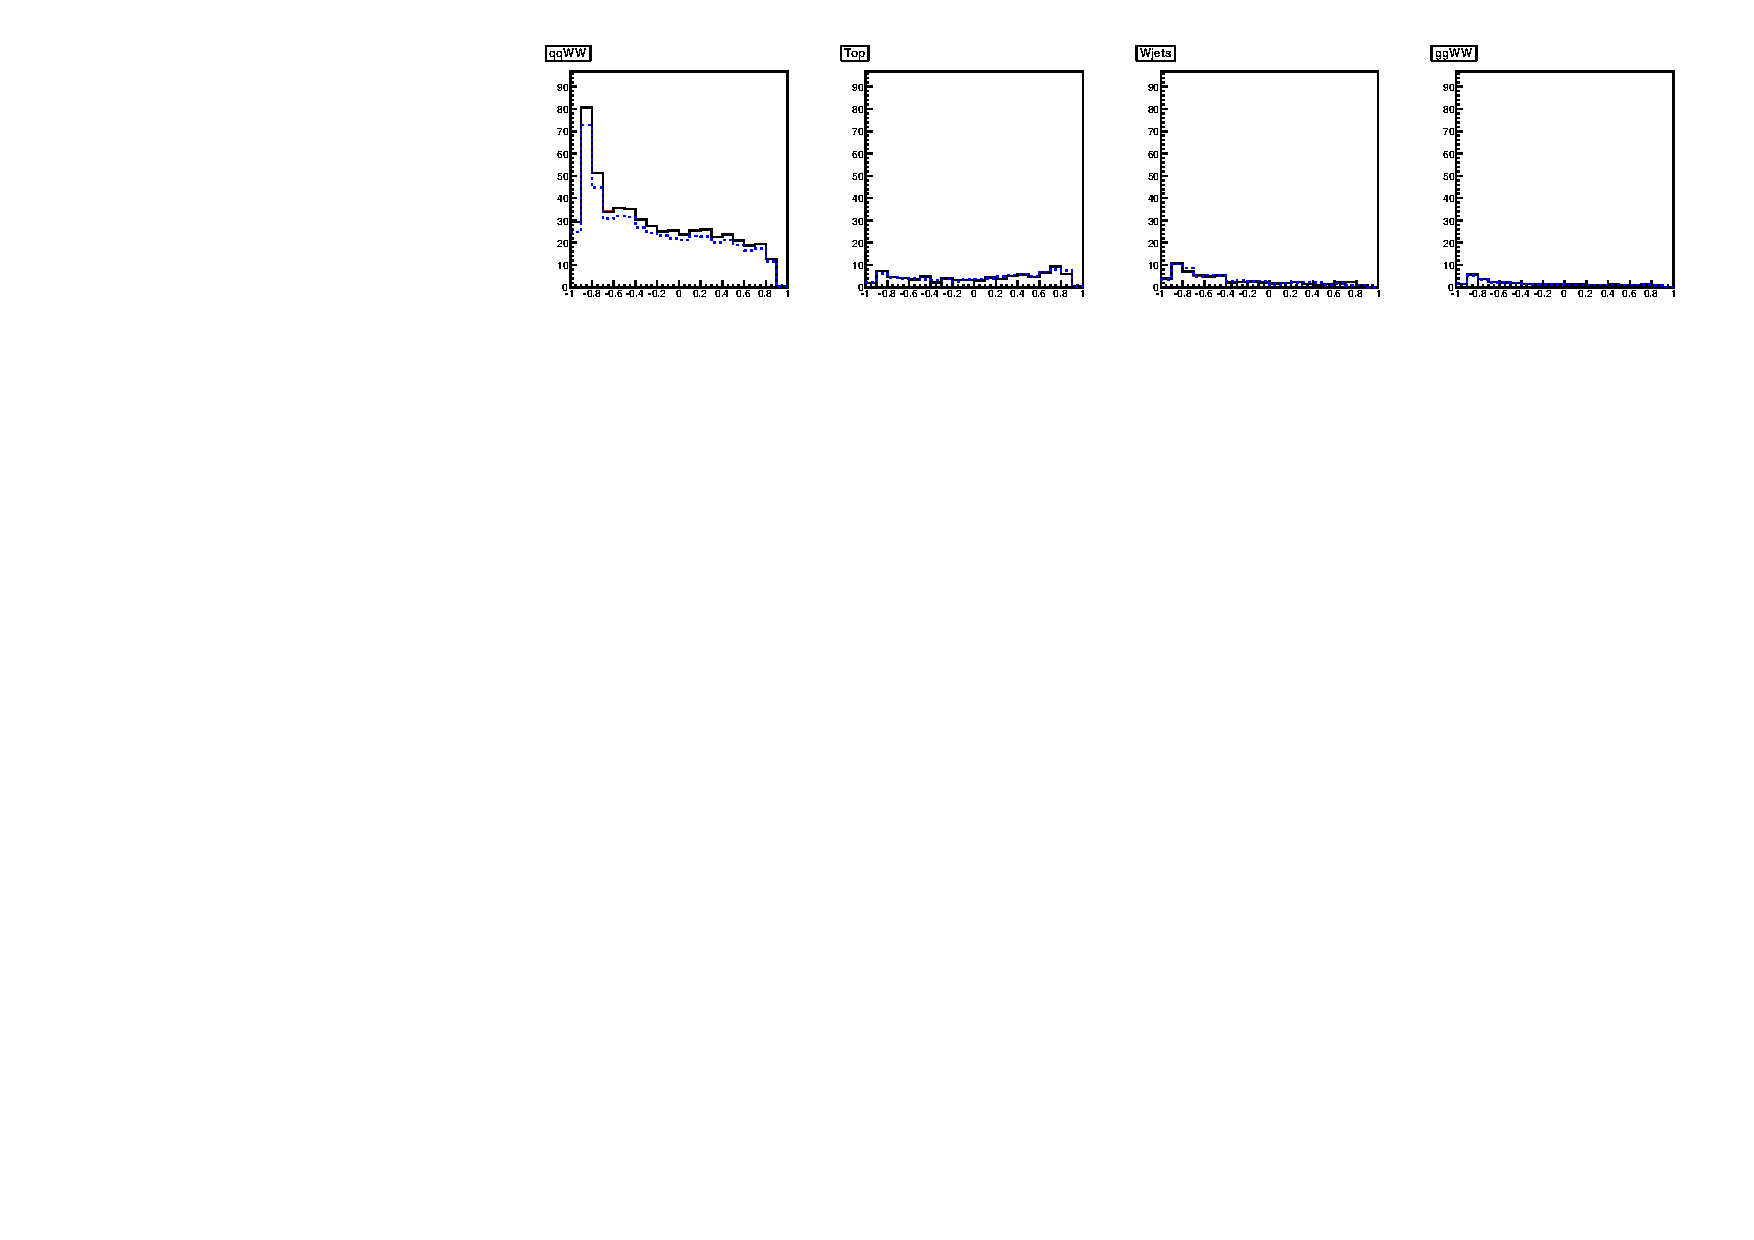
\includegraphics[width=1.0\textwidth]{figures/fits/bdt2_350_n0of.pdf}}\\
\subfigure[$ee$/$\mu\mu$ 0-Jet]{
\centering
\label{subfig:bdt2_350_n0sf}
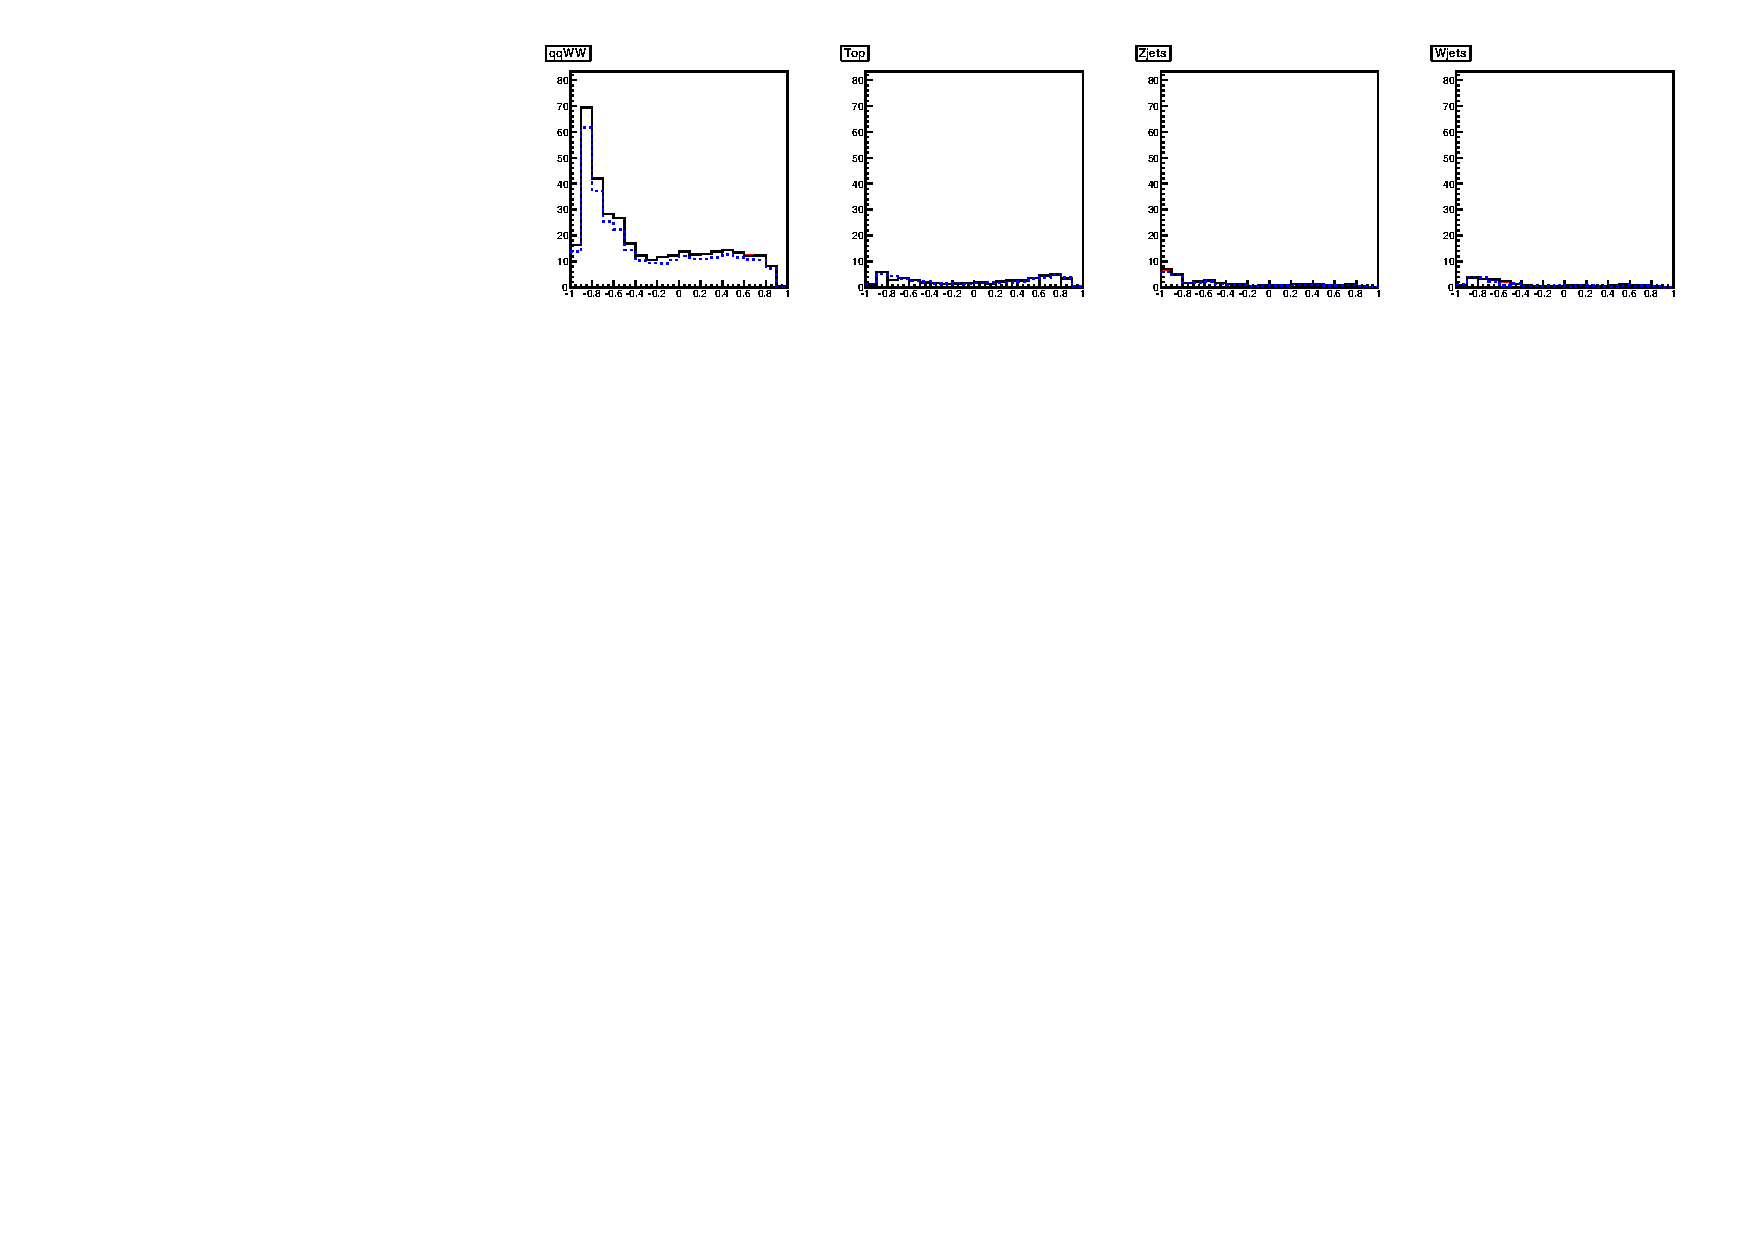
\includegraphics[width=1.0\textwidth]{figures/fits/bdt2_350_n0sf.pdf}}
\subfigure[$e\mu$ 1-Jet]{
\centering
\label{subfig:bdt2_350_n1of}
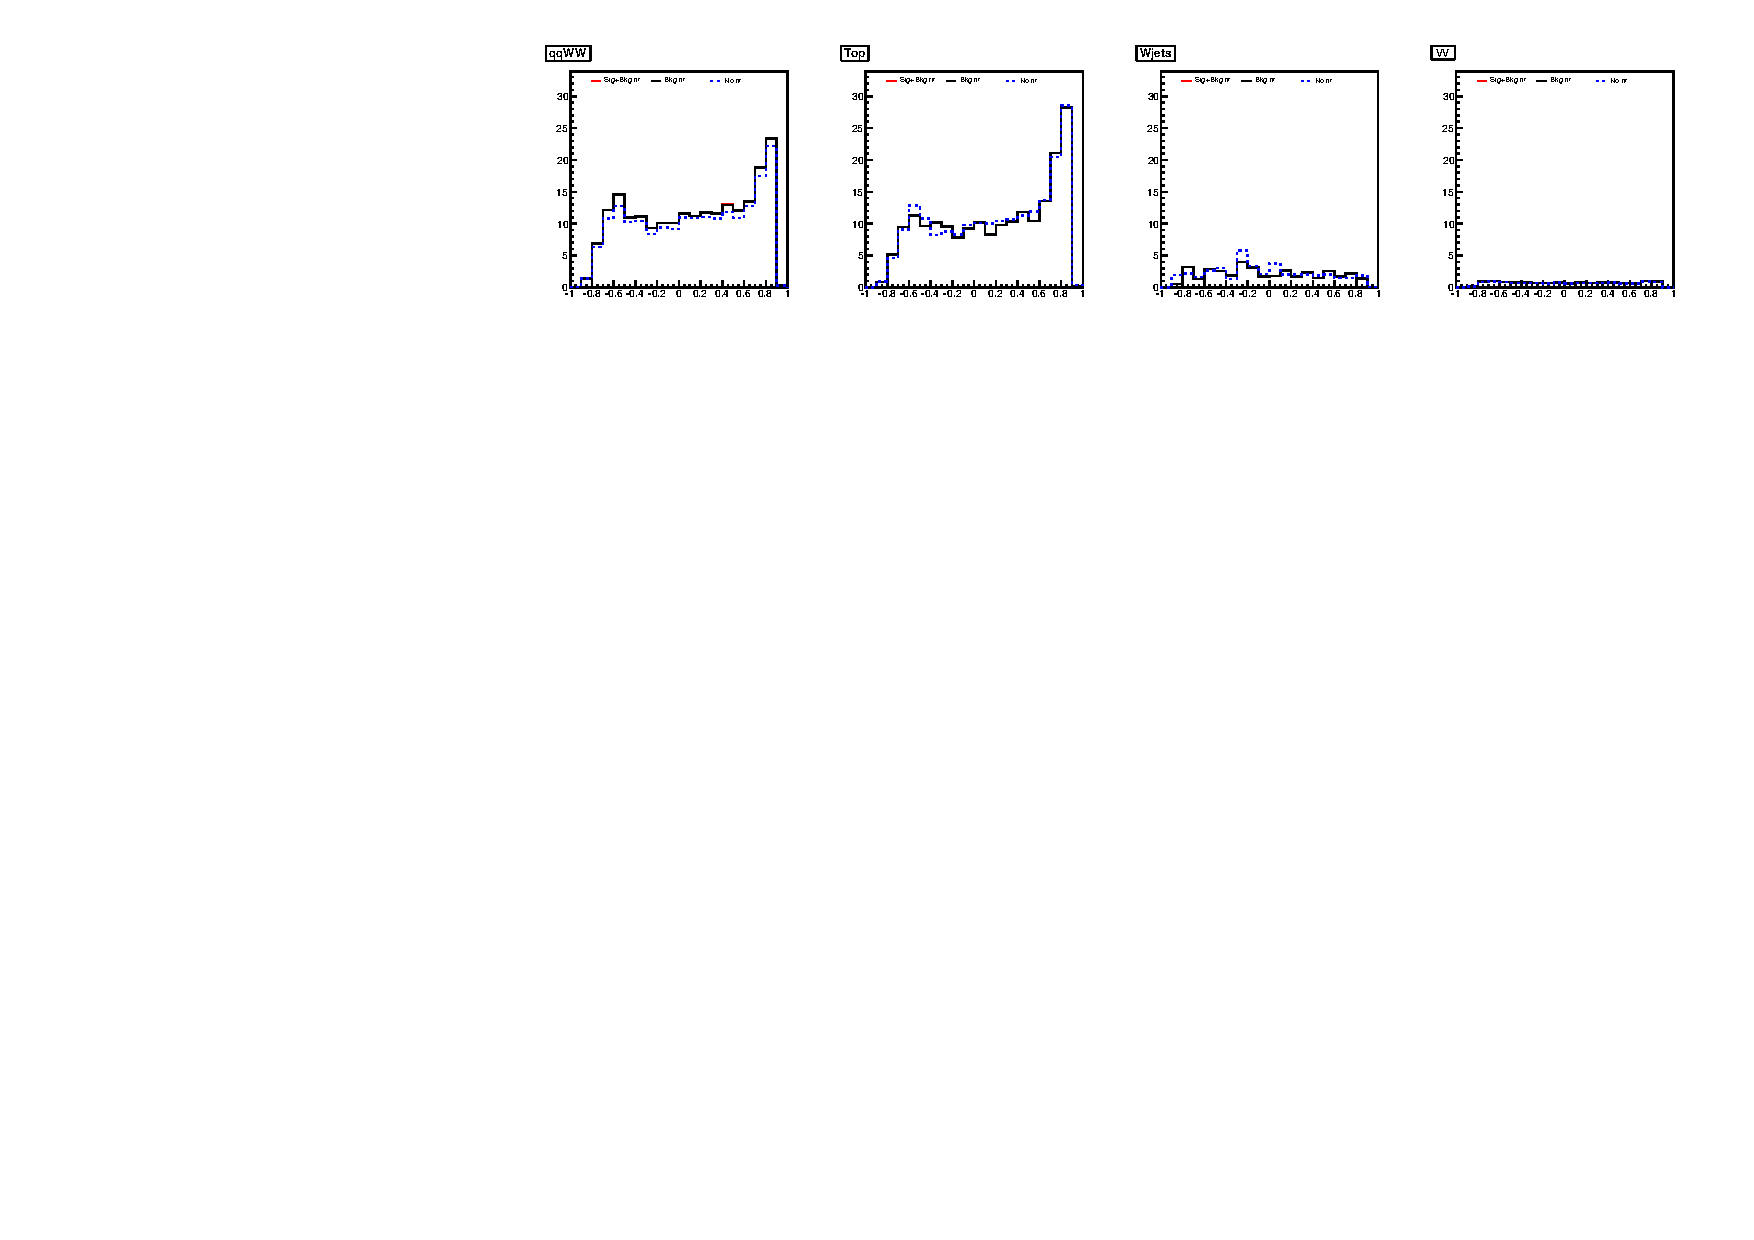
\includegraphics[width=1.0\textwidth]{figures/fits/bdt2_350_n1of.pdf}}\\
\subfigure[$ee$/$\mu\mu$ 1-Jet]{
\centering
\label{subfig:bdt2_350_n1sf}
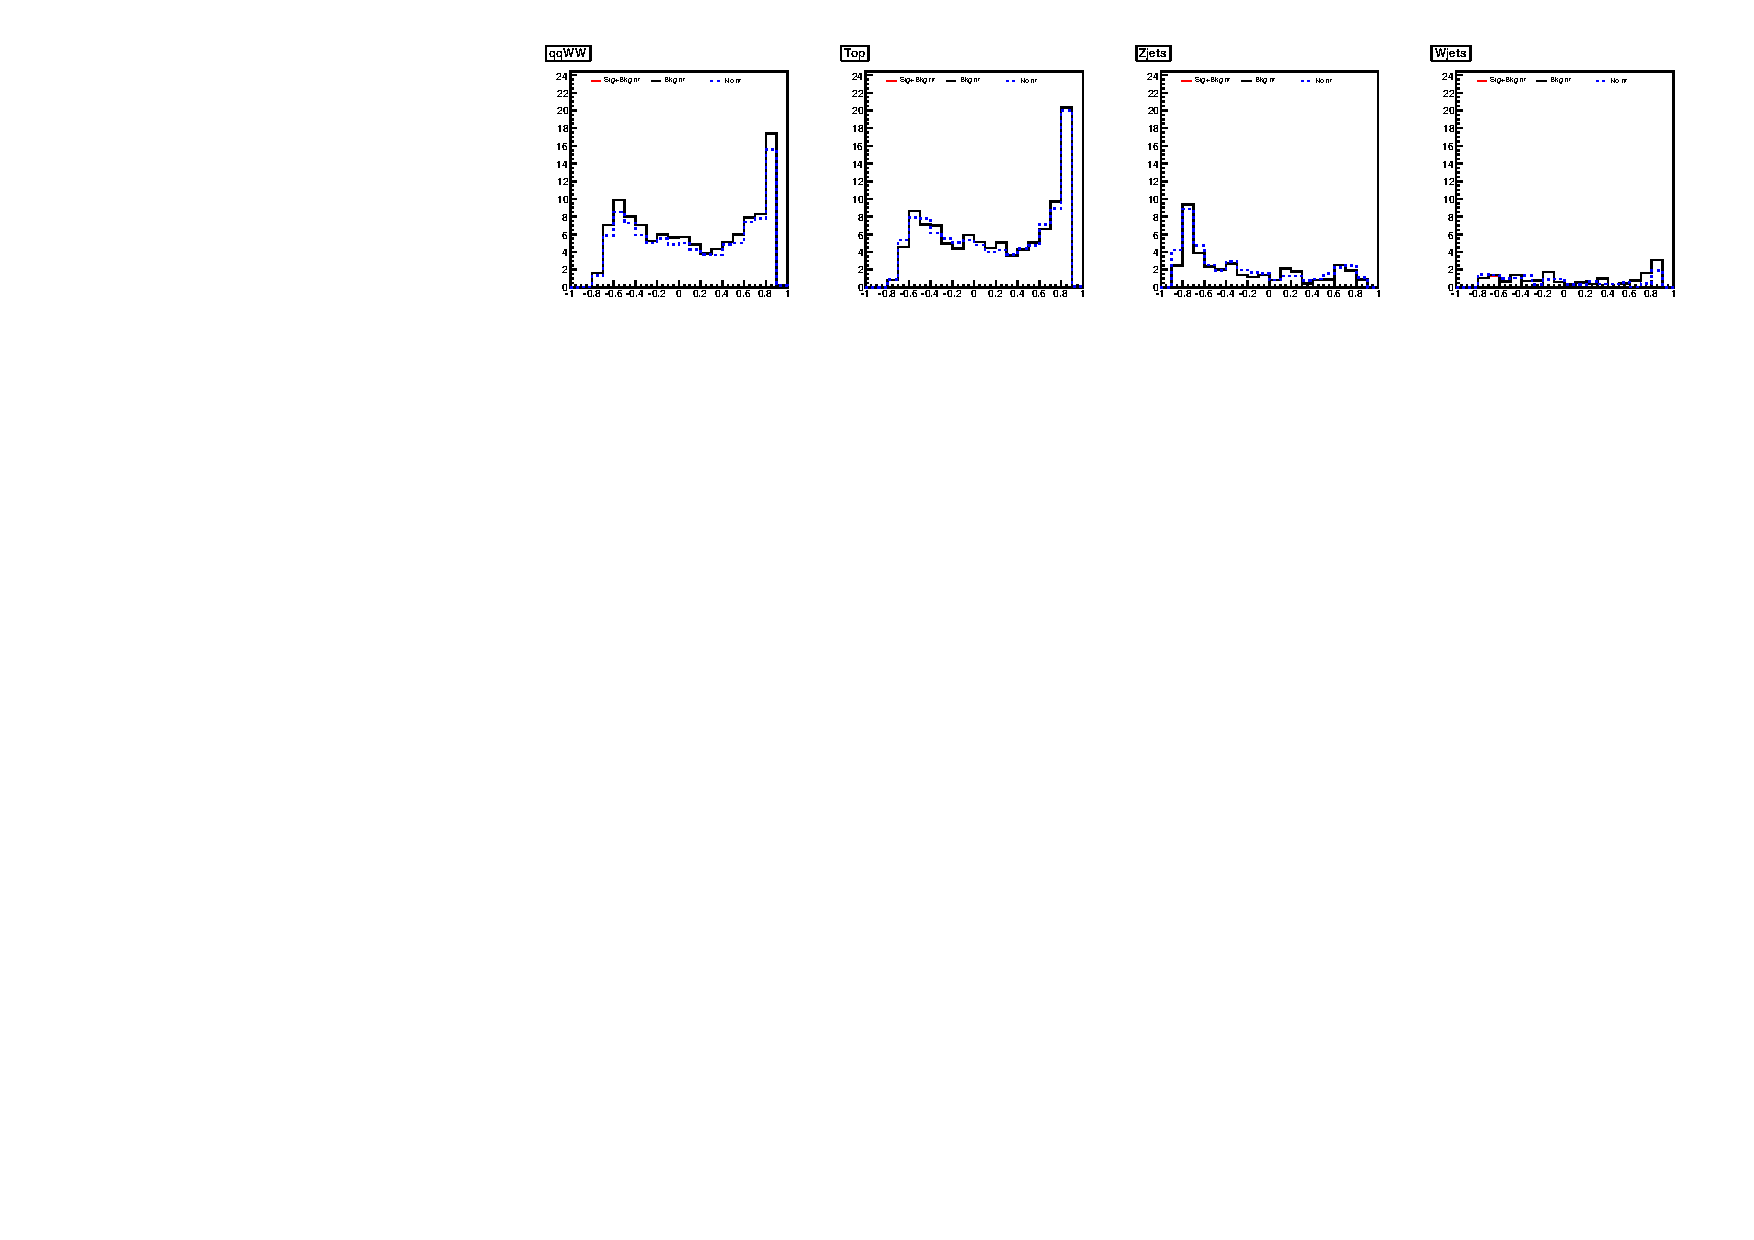
\includegraphics[width=1.0\textwidth]{figures/fits/bdt2_350_n1sf.pdf}}
\caption{
MVA output distributions for dominant background contributions for
Higgs 350~\GeV\ without fitting (nominal), background fit (signal is
set to zero) and signal+background fit (signal is floating in the
fit).}
\label{fig:bdt2_350}
\end{figure}

\begin{figure}[!hbtp]
\centering
\subfigure[$e\mu$ 0-Jet]{
\centering
\label{subfig:bdt2_400_n0of}
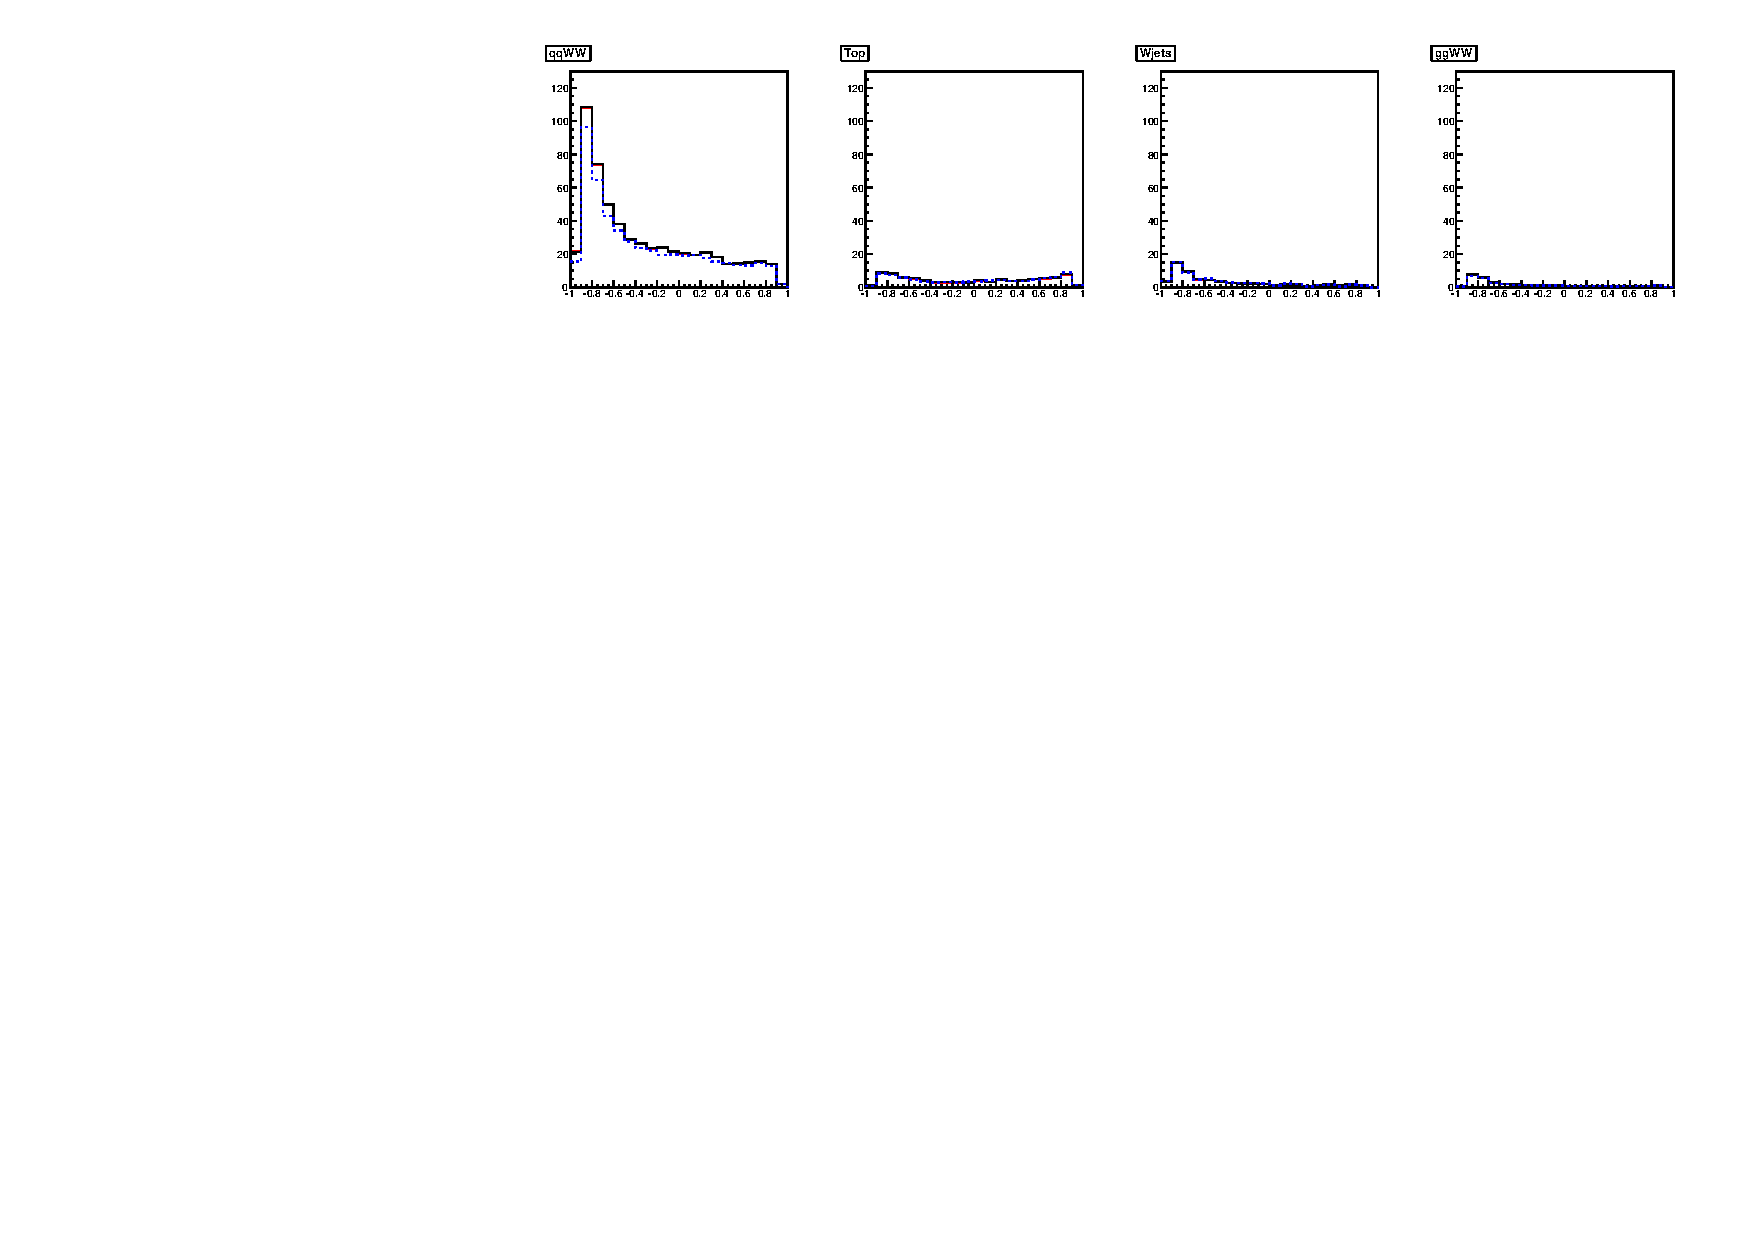
\includegraphics[width=1.0\textwidth]{figures/fits/bdt2_400_n0of.pdf}}\\
\subfigure[$ee$/$\mu\mu$ 0-Jet]{
\centering
\label{subfig:bdt2_400_n0sf}
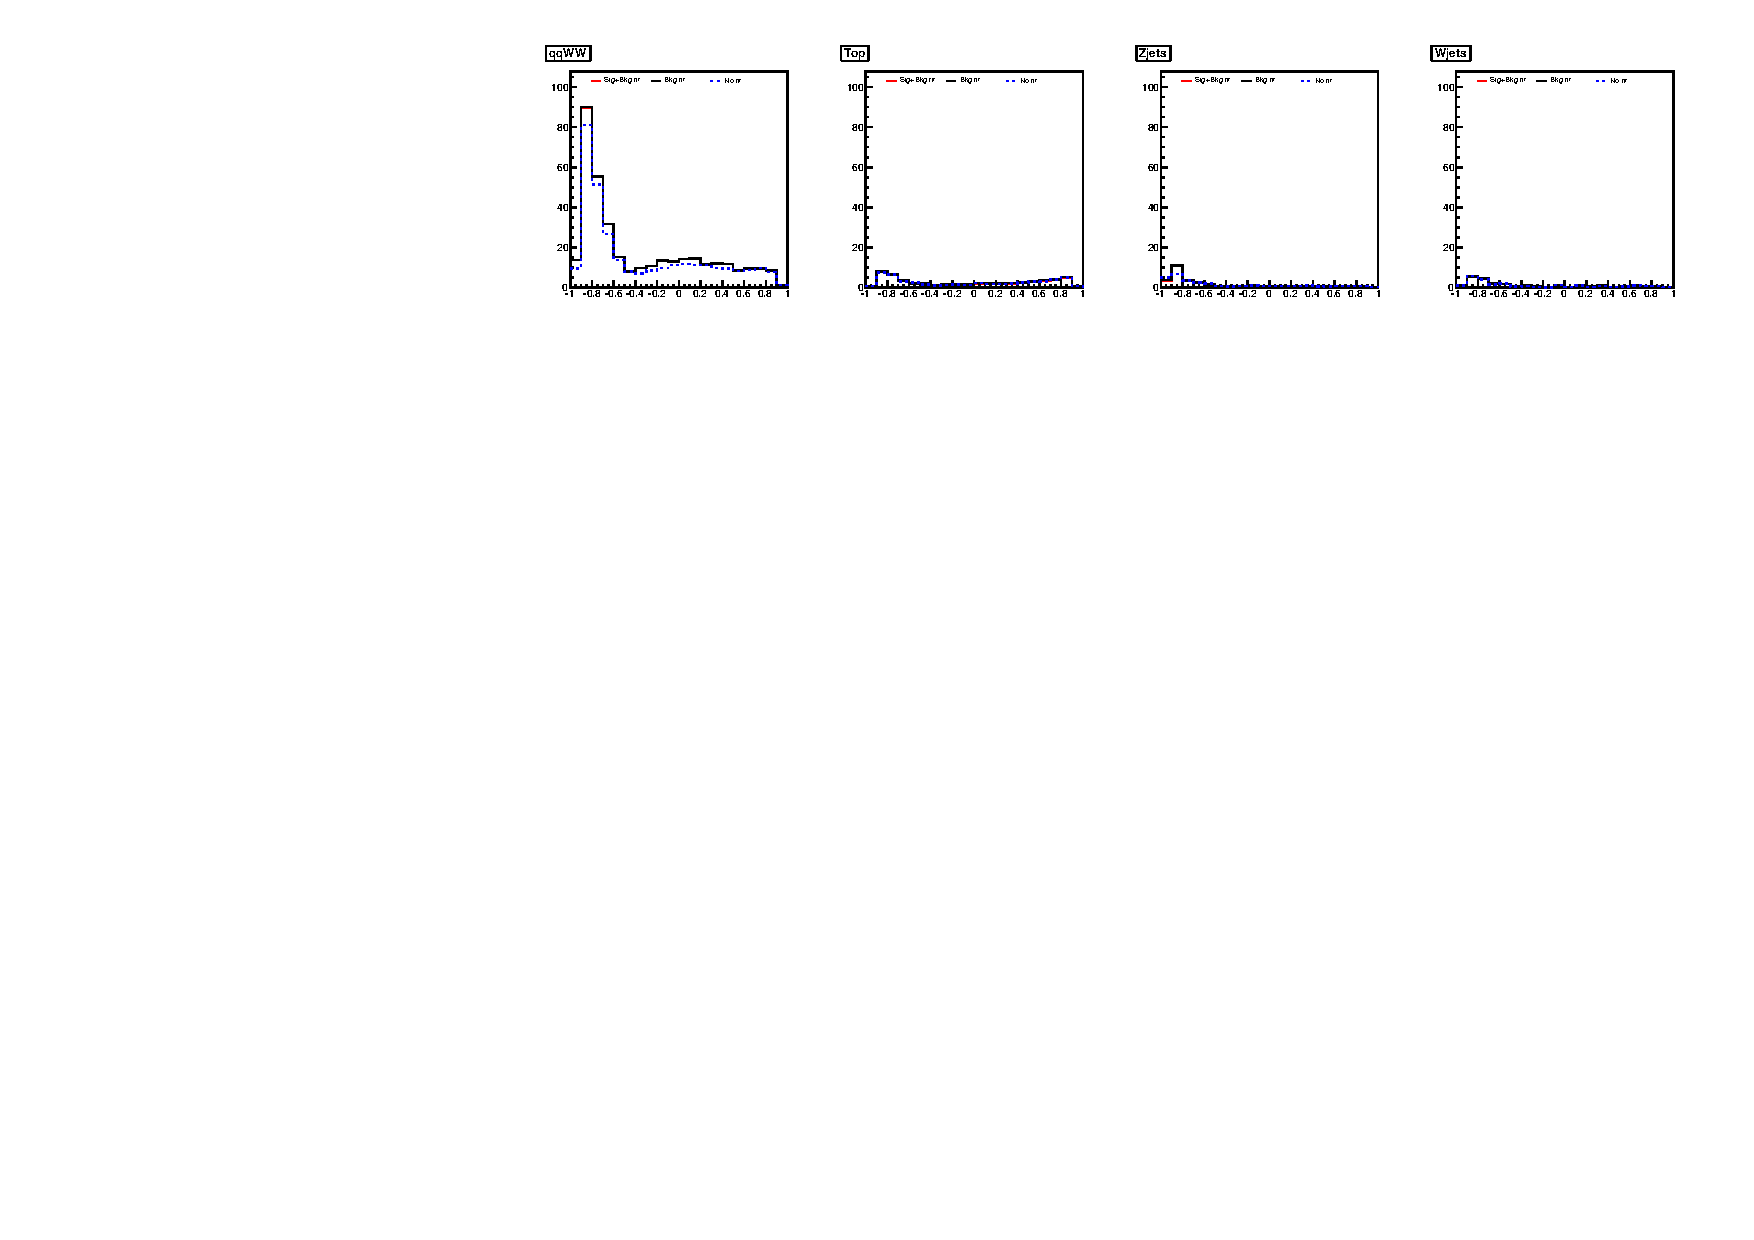
\includegraphics[width=1.0\textwidth]{figures/fits/bdt2_400_n0sf.pdf}}
\subfigure[$e\mu$ 1-Jet]{
\centering
\label{subfig:bdt2_400_n1of}
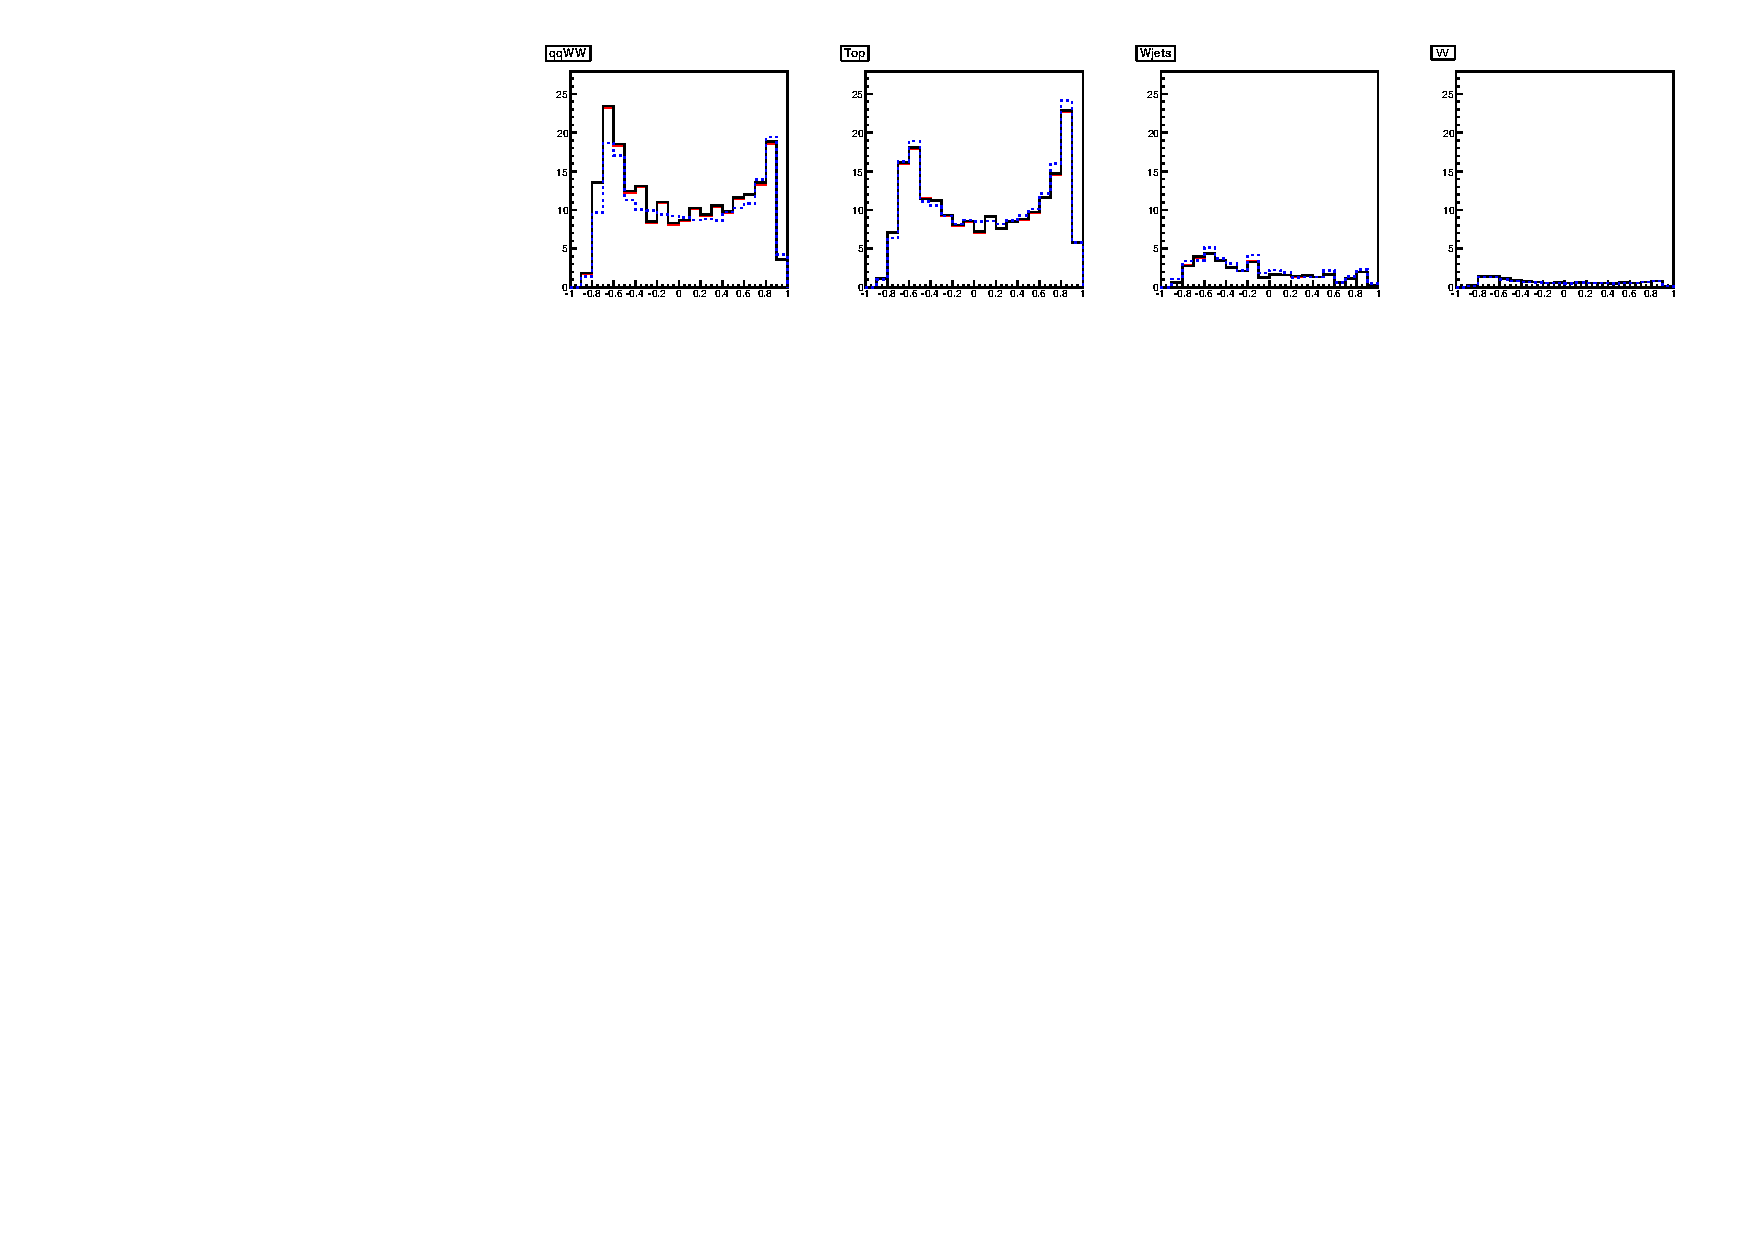
\includegraphics[width=1.0\textwidth]{figures/fits/bdt2_400_n1of.pdf}}\\
\subfigure[$ee$/$\mu\mu$ 1-Jet]{
\centering
\label{subfig:bdt2_400_n1sf}
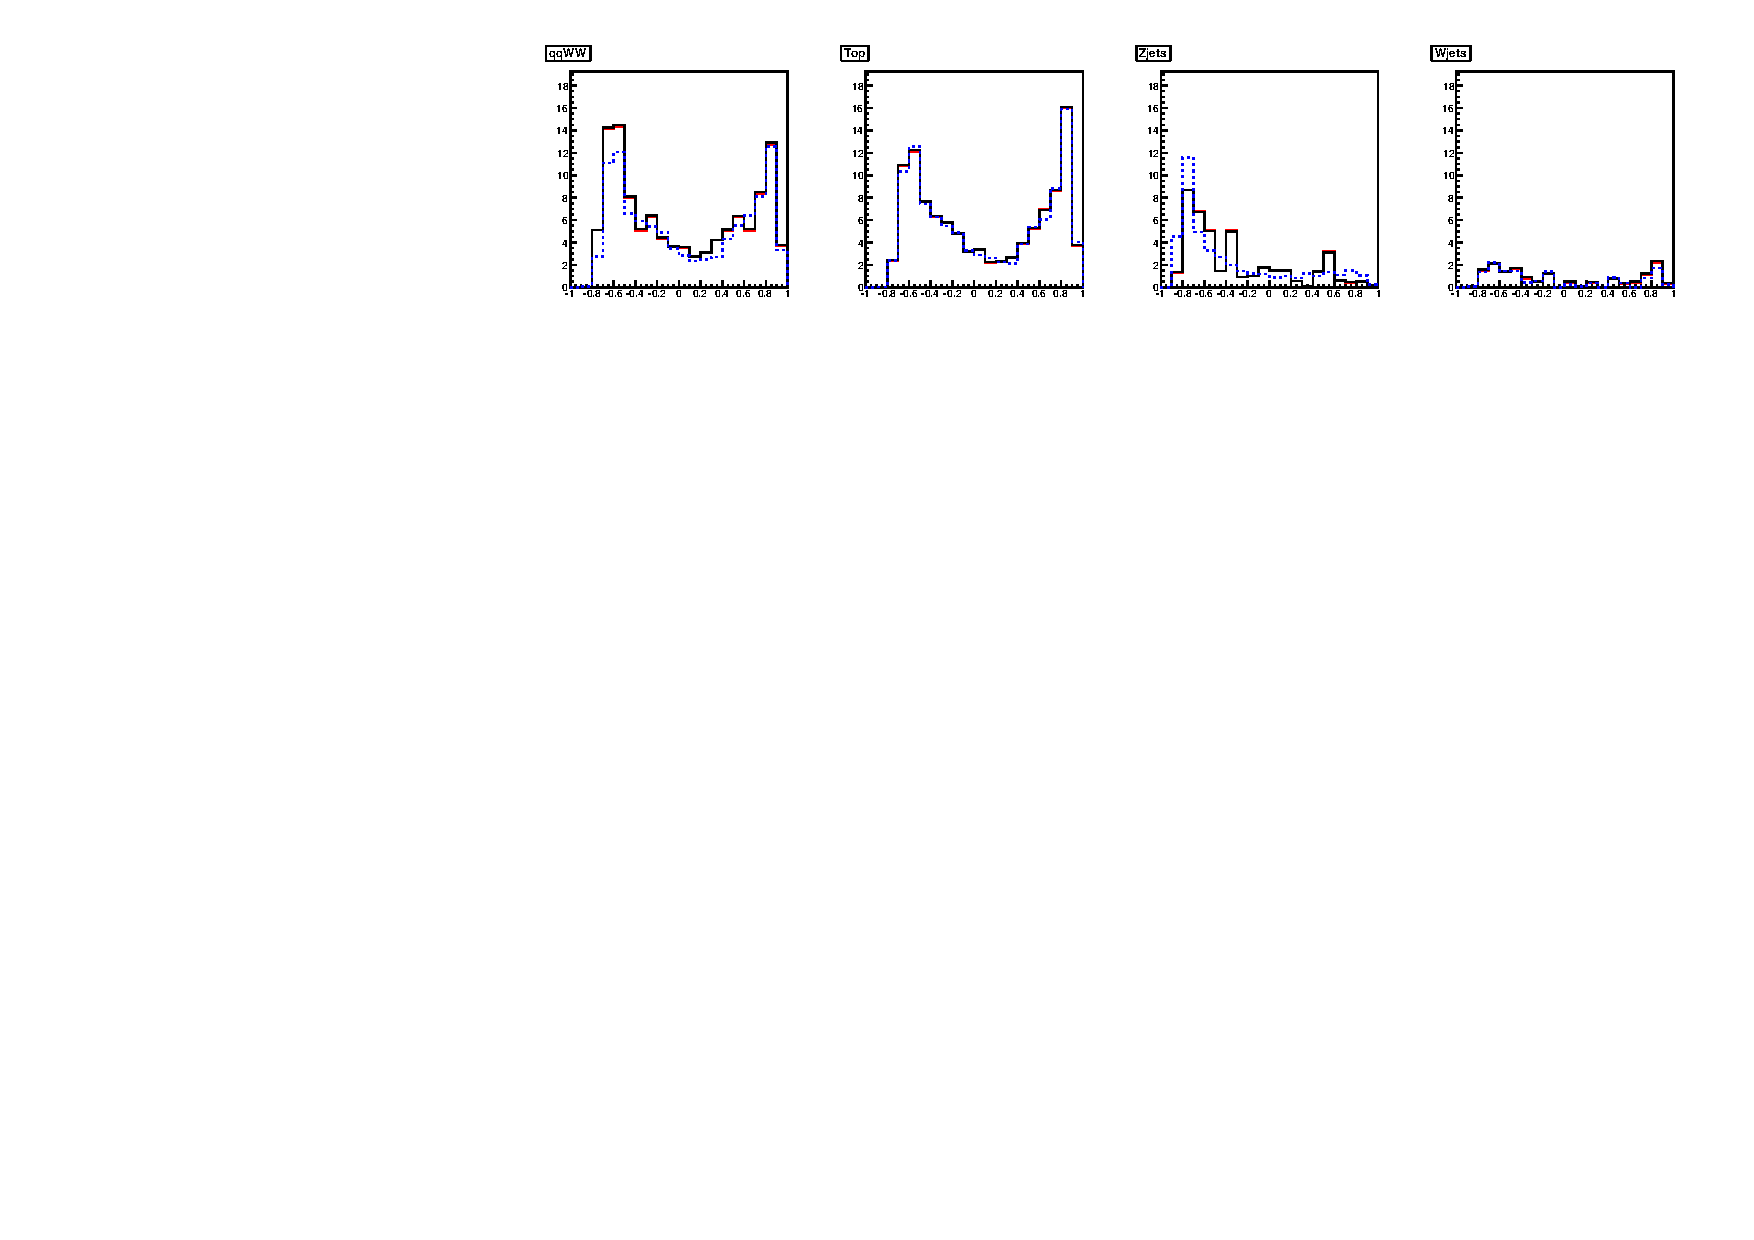
\includegraphics[width=1.0\textwidth]{figures/fits/bdt2_400_n1sf.pdf}}
\caption{
MVA output distributions for dominant background contributions for
Higgs 400~\GeV\ without fitting (nominal), background fit (signal is
set to zero) and signal+background fit (signal is floating in the
fit).}
\label{fig:bdt2_400}
\end{figure}
